\documentclass[11pt,letterpaper]{article}
\pdfoutput=1
\usepackage{jheppub}

\usepackage[utf8]{inputenc}

\usepackage{color}
\usepackage{graphicx}
\usepackage{tabularx}
\usepackage{xspace}

\usepackage{verbatim}
\usepackage{amsmath}
\usepackage{amssymb}
\usepackage[caption=false]{subfig}
\usepackage{url}
\usepackage{bbold}
\usepackage{slashed}
\usepackage{array}

\usepackage{multirow}
\usepackage{threeparttable}
\usepackage{paralist}

\newcommand{\GeV}{\text{GeV}}
\newcommand{\TeV}{\text{TeV}}
\newcommand{\SO}{\text{SO}}
\newcommand{\SU}{\text{SU}}
\newcommand{\SM}{\text{SM}}

\newcommand{\U}{\text{U}}
\newcommand{\CKM}{\text{CKM}}
\newcommand{\eff}{\text{eff}}

\newcommand{\genang}[2]{{\lambda^{#1}_{#2}}}


\newcommand{\ev}{\text{event}}
\newcommand{\jet}{\text{jet}}
\newcommand{\jets}{\text{jets}}
\newcommand{\subj}{\text{subjet}}
\newcommand{\subjs}{\text{subjets}}
\newcommand{\cut}{\text{cut}}
\newcommand{\trim}{\text{trim}}
\newcommand{\Ecut}{E_{{\rm cut}}}

\newcommand{\dichroic}{\text{dichroic}}
\newcommand{\groomed}{\text{groomed}}

\newcommand{\ptc}{p_{T{\rm cut}}}
\newcommand{\ptsubc}{p_{T{\rm subcut}}}

\newcommand{\sub}{\text{sub}}
\newcommand{\miss}{\text{miss}}

\newcommand{\pythia}{\textsc{Pythia~8}\xspace}
\newcommand{\herwig}{\textsc{Herwig++}\xspace}
\newcommand{\eventtwo}{\textsc{Event2}\xspace}
\newcommand{\vincia}{\textsc{Vincia}\xspace}
\newcommand{\sherpa}{\textsc{Sherpa}\xspace}

\newcommand{\FastJet}{\textsc{FastJet}\xspace}
\newcommand{\MadGraph}{\textsc{MadGraph}\xspace}

\newcommand{\df}{\text{d}}
\newcommand{\vev}[1]{\langle #1 \rangle}


\DeclareRobustCommand{\Sec}[1]{Sec.~\ref{#1}}
\DeclareRobustCommand{\Secs}[2]{Secs.~\ref{#1} and \ref{#2}}
\DeclareRobustCommand{\Secss}[3]{Secs.~\ref{#1}, \ref{#2}, and \ref{#3}}
\DeclareRobustCommand{\App}[1]{App.~\ref{#1}}
\DeclareRobustCommand{\Tab}[1]{Table~\ref{#1}}
\DeclareRobustCommand{\Tabs}[2]{Tables~\ref{#1} and \ref{#2}}
\DeclareRobustCommand{\Fig}[1]{Fig.~\ref{#1}}
\DeclareRobustCommand{\Figs}[2]{Figs.~\ref{#1} and \ref{#2}}
\DeclareRobustCommand{\Figss}[3]{Figs.~\ref{#1}, \ref{#2}, and \ref{#3}}
\DeclareRobustCommand{\Eq}[1]{Eq.~(\ref{#1})}
\DeclareRobustCommand{\Eqs}[2]{Eqs.~(\ref{#1}) and (\ref{#2})}
\DeclareRobustCommand{\Eqss}[3]{Eqs.~(\ref{#1}), (\ref{#2}), and (\ref{#3})}
\DeclareRobustCommand{\Ref}[1]{Ref.~\cite{#1}}
\DeclareRobustCommand{\Refs}[1]{Refs.~\cite{#1}}

\newcommand{\be}{\begin{equation}}
\newcommand{\ee}{\end{equation}}
\newcommand{\nn}{\nonumber}

\renewcommand{\textfraction}{0.10}
\renewcommand{\topfraction}{0.90}
\renewcommand{\bottomfraction}{0.90}
\renewcommand{\floatpagefraction}{0.65}

%% Reference commands %%
\newcommand{\mb}[1]{\boldsymbol{#1}}
\newcommand{\bm}[1]{\boldsymbol{#1}}
\newcommand{\mbo}[1]{\boldsymbol{\overline{#1}}}

\usepackage{xspace}


\def\Tr{\mathop{\rm Tr}}
\newcommand{\rep}[1]{\mathbf{#1}}
\newcommand{\conjrep}[1]{\overline{\mathbf{#1}}}


\renewcommand{\a}{\alpha}
\renewcommand{\b}{\beta}
\newcommand{\e}{\epsilon}
\newcommand{\D}{\Delta}
\renewcommand{\l}{\lambda}
\renewcommand{\th}{\theta}
\newcommand{\bq}{\bar{q}}
\newcommand{\zcut}{z_{\rm cut}}

\newcommand{\IZ}{\mathbb{Z}}
\newcommand{\cD}{\mathcal{D}}
\newcommand{\cL}{\mathcal{L}}
\newcommand{\cR}{\mathcal{R}}
\newcommand{\cF}{\mathcal{F}}
\newcommand{\cI}{\mathcal{I}}
\newcommand{\cK}{\mathcal{K}}
\newcommand{\beq}{\begin{eqnarray}}
\newcommand{\eeq}{\end{eqnarray}}

\newcommand{\F}{\mathcal{F}}
\newcommand{\Ft}{\widetilde{\mathcal{F}}}
\newcommand{\G}{\mathcal{G}}
\newcommand{\Gt}{\widetilde{\mathcal{G}}}
\newcommand{\HH}{\mathcal{H}}
\newcommand{\HHt}{\widetilde{\mathcal{H}}}
\newcommand{\ord}[1]{\mathcal{O}\!\left(#1\right)}

\newcommand*\numcircledmod[1]{#1 \!\!\! \bigcirc}

\newcommand{\Njet}{\widetilde{N}_{\rm jet}}
\newcommand{\dN}[1]{\Delta_{#1}}
\newcommand{\dNpm}{\Delta_{2\pm}}
\newcommand{\dNp}{\Delta_{2+}}
\newcommand{\dNm}{\Delta_{2-}}
\newcommand{\dNtm}{\Delta_{3-}}

\newcommand{\cT}{\mathcal{T}}
\newcommand{\as}{\alpha_s}
\renewcommand{\angle}{\theta}


\newcommand{\ecf}[2]{e_{#1}^{(#2)}} 
\newcommand{\ecfnobeta}[1]{e_{#1}} 

\newcommand{\ecfvar}[3]{{_{#1}e_{#2}^{(#3)}}} 
\newcommand{\ecfvarnobeta}[2]{{_{#1}e_{#2}}} 

\newcommand{\Dobs}[2]{D_{#1}^{(#2)}} 
\newcommand{\Dobsnobeta}[1]{D_{#1}} 

\newcommand{\Xobs}[2]{X_{#1}^{(#2)}} 

\newcommand{\Cobs}[2]{C_{#1}^{(#2)}} 
\newcommand{\Cobsnobeta}[1]{C_{#1}} 

\newcommand{\Nsub}[2]{\tau_{#1}^{(#2)}}
\newcommand{\Nsubnobeta}[1]{\tau_{#1}}


%\newcommand{\pythia}[1]{\textsc{Pythia\xspace #1}}
\newcommand{\madgraph}[1]{\textsc{MadGraph5\xspace #1}}
\newcommand{\fastjet}[1]{\textsc{FastJet\xspace #1}}
%\newcommand{\herwig}[1]{\textsc{Herwig\xspace #1}}
\newcommand{\herwigpp}[1]{\textsc{Herwig++\xspace #1}}
%\newcommand{\vincia}[1]{\textsc{Vincia\xspace #1}}
\newcommand{\nlojet}{\textsc{NLOJet++}}
%\newcommand{\sherpa}{\textsc{Sherpa}}
\newcommand{\ariadne}{\textsc{Ariadne}}
\newcommand{\geneva}{\textsc{Geneva}}
\newcommand{\dire}{\textsc{Dire}}




%\definecolor{darkgreen}{rgb}{0,0.5,0}
%\newcommand{\jdt}[1]{\textbf{\textcolor{darkgreen}{(#1 --jdt)}}}

%\definecolor{darkblue}{rgb}{0,0,0.5}
%\newcommand{\gs}[1]{\textbf{\textcolor{darkblue}{(#1 --gs)}}}

\definecolor{llblue}{rgb}{0,0.5,1.0}
\newcommand{\ijm}[1]{\textbf{\textcolor{llblue}{(#1 --ijm)}}}


\definecolor{darkgreen}{rgb}{0,0.6,0.0}
\newcommand{\gs}[1]{\textbf{\textcolor{darkgreen}{(#1 --gs)}}}





\begin{document}


%\title{Performance versus Robustness for Two-Prong Jet Substructure}
\title{Performance versus Robustness:\\
Two-Prong Substructure Taggers for the LHC}

\author[a]{Disha Bhatia,}
\author[a]{Reina Camacho,}
\author[a]{Grigorios Chachamis,}
\author[a]{Suman Chatterjee,}
\author[a]{Frederic Dreyer,}
\author[a]{Deepak Kar,}
\author[a]{Peter Loch,}
\emailAdd{loch@physics.arizona.edu}
\author[a]{Ian Moult,}
\emailAdd{ianmoult@lbl.gov}
\author[a]{Ben Nachman,}
\emailAdd{bpnachman@lbl.gov}
\author[a]{Andreas Papaefstathiou,}
\author[a]{Tousik Samui,}
\author[a]{Andrzej Siodmok,}
\author[a]{Gregory Soyez,}
\emailAdd{gregory.soyez@ipht.fr}
\author[a]{and Jesse Thaler}
\emailAdd{jthaler@mit.edu}

\affiliation[a]{Les Houches}
\affiliation[5]{Center for Theoretical Physics, Massachusetts Institute of Technology, Cambridge, MA 02139, USA}
\affiliation[3]{Berkeley Center for Theoretical Physics, University of California, Berkeley, CA 94720, USA}
\affiliation[4]{Theoretical Physics Group, Lawrence Berkeley National Laboratory, Berkeley, CA 94720, USA}


\abstract{The ability to robustly identify boosted hadronically
  decaying resonances plays a central role at the LHC, both in
  searches for new physics, as well as for probing the Standard Model
  in extreme regions of phase space. While a variety of powerful and
  theoretically well understood approaches exist, different behavior
  is \gs{behaviours are?} often observed in realistic experimental
  contexts, and the different experiments use different strategies,
  without a well understood motivation. In this paper we perform a
  systematic study contrasting the robustness and performance of
  different theoretical approaches to designing jet substructure
  observables. These include the standard observables $\tau_{21}$,
  $D_2$, and $N_2$, and grooming strategies, currently used by the
  experiments, as well as generalizations, based on the idea of
  dichroic ratios, which are designed to simultaneously maximize both
  robustness and performance. For signal jets, we focus on robustness
  to the polarization of the sample, while for QCD jets, we focus on
  theoretical robustness to non-perturbative effects, and experimental
  robustness to detector effects. Additionally, we identify strategies
  to tag the polarization of hadronically decaying bosons. We discuss
  the different choices used by CMS and ATLAS in the context of
  robustness vs. performance, and make recommendations for future
  tagging strategies to ensure robust procedures based on sound
  theoretical organizing principles. Additionally, we introduce
  reliable metrics for quantifying robustness and performance for
  substructure observables.

}

\maketitle

%%%%%%%%%%%%%%%%%%%%%%%%%%%%%%%%%%%%%%%
\section{Introduction}\label{sec:intro}
%%%%%%%%%%%%%%%%%%%%%%%%%%%%%%%%%%%%%%%

\ijm{update citations, and include the review}

With the ever increasing LHC dataset, we are able to probe the Standard Model and search for physics beyond the Standard Model in increasingly extreme regions of phase space. Well understood theoretical observables that are sensitive to such extreme regions of phase space are therefore playing an increasingly important role at the LHC. One of the most exciting new approaches which has emerged at the LHC are tools from jet substructure, which allow for the identification of boosted hadronically decaying particles within jets by a detailed study of their radiation pattern. Techniques from jet substructure have now been widely used for Standard Model measurements \cite{Chatrchyan:2012sn,CMS:2013cda,Aad:2015cua,Aad:2015lxa,ATLAS-CONF-2015-035,Aad:2015rpa,Aad:2015hna,ATLAS-CONF-2016-002,ATLAS-CONF-2016-039,ATLAS-CONF-2016-034,CMS-PAS-TOP-16-013,CMS-PAS-HIG-16-004}, as well as for searches of new physics  \cite{CMS:2011bqa,Fleischmann:2013woa,Pilot:2013bla,TheATLAScollaboration:2013qia,Chatrchyan:2012ku,CMS-PAS-B2G-14-001,CMS-PAS-B2G-14-002,Khachatryan:2015axa,Khachatryan:2015bma,Aad:2015owa,Aaboud:2016okv,Aaboud:2016trl,Aaboud:2016qgg,ATLAS-CONF-2016-055,ATLAS-CONF-2015-071,ATLAS-CONF-2015-068,CMS-PAS-EXO-16-037,CMS-PAS-EXO-16-040,Khachatryan:2016mdm,CMS-PAS-HIG-16-016,CMS-PAS-B2G-15-003,CMS-PAS-EXO-16-017}.\footnote{More LHC studies using jet substructure can be found at \url{https://twiki.cern.ch/twiki/bin/view/AtlasPublic} and \url{http://cms-results.web.cern.ch/cms-results/public-results/publications/}.} 


 
 With the growing importance of jet substructure techniques, there has been a significant effort by both the theory and experimental communities to develop a more detailed understanding of the theoretical and experimental behavior of jet substructure observables. On the theory side, this has been pursued through explicit calculations \cite{Feige:2012vc,Field:2012rw,Dasgupta:2013ihk,Dasgupta:2013via,Larkoski:2014pca,Dasgupta:2015yua,Seymour:1997kj,Li:2011hy,Larkoski:2012eh,Jankowiak:2012na,Chien:2014nsa,Chien:2014zna,Isaacson:2015fra,Krohn:2012fg,Waalewijn:2012sv,Larkoski:2014tva,Procura:2014cba,Bertolini:2015pka,Bhattacherjee:2015psa,Larkoski:2015kga,Dasgupta:2015lxh,Frye:2016okc,Frye:2016aiz,Kang:2016ehg,Hornig:2016ahz,Marzani:2017mva}, scaling arguments \cite{Walsh:2011fz,Larkoski:2014gra,Larkoski:2014zma} and machine learning \cite{Cogan:2014oua,deOliveira:2015xxd,Almeida:2015jua,Baldi:2016fql,Guest:2016iqz,Conway:2016caq,Barnard:2016qma} approaches. On the experimental side, there have been detailed studies of the behavior of substructure observables in data, and their interplay with experimental realities, such as detector resolution and pile up. Summaries can be found in \cite{Abdesselam:2010pt,Altheimer:2012mn,Altheimer:2013yza,Adams:2015hiv}.

As a result of these efforts, there now exist a number of theoretically well motivated jet substructure tools. For tagging hadronically decaying $W/Z/H$ bosons, which decay primarily to jets with two well resolved prongs, or subjets, a variety of powerful two-prong taggers have been developed.  Modern two-prong taggers typically consist of two ingredients: a groomer and a jet shape observable.
For jet shapes, it is well understood how to organize and study their
behavior using power counting \cite{Larkoski:2014gra}. A variety of
different classes of observables exist, for example the Energy
correlation functions \cite{Larkoski:2013eya} and N-subjettiness
observables \cite{Thaler:2010tr,Thaler:2011gf}, and their relation is
understood. The behavior of groomers is also now well understood, and
their exist groomers with nice experimental and theoretical properties
\cite{Dasgupta:2013ihk,Larkoski:2014wba}. However, despite the
theoretical understanding of the behavior of the observables, it is
not always clear how this translates to experimental reality, due to
the presence of hadronization, underlying event, detector effects and
pile up. Indeed, the different experiments have settled on different
tagging combinations. For grooming, which removes low energy
contamination,  ATLAS using trimming \cite{Krohn:2009th}, while CMS
uses soft drop\cite{Larkoski:2014wba}\gs{``while CMS uses the Modified
  MassDrop Tagger~\cite{Dasgupta:2013ihk}''}. For observable, ATLAS uses $D_2$ \cite{Larkoski:2014gra,Larkoski:2015kga}, while CMS uses $N$-subjettiness ratio $\tau_{2,1}$ \cite{Thaler:2010tr,Thaler:2011gf}, or $N_2$ \cite{Moult:2016cvt} with DDT \cite{Dolen:2016kst}. It is not clear if this is driven by differences in the detectors, or an optimization with respect to different criteria, samples, or modelling, as it is generally not well understood the extent to which the substructure observables are robust to such issues.





In this paper we perform a comprehensive study of performance and robustness for two-prong tagging techniques using a theoretical organization into different categories of tagging strategies based on the idea of dichroic observables \cite{Salam:2016yht}, which generalize ratio observables to allow hybrid combinations of groomed and ungroomed shapes. These categories contain as special instances all the familiar observables used by the experiments, as well as new observables, such as dichroic versions of the $N_2$ and $D_2$ observables. We therefore place the ATLAS and CMS strategies as specific examples of broader classes of theoretical approaches for tagging two-prong substructure, about which we can draw general conclusions regarding robustness and performance.
%We discuss the physics associated with each of the different classes of approaches, and consider families characterized by different parameters within each of these classes. This allows us to optimize within each of these classes, as well as to compare the behavior within different classes.


The primary focus of this study is the interplay between robustness and performance. Here robustness refers to modifications of the substructure observables as different physics aspects are added. In particular, we consider robustness to non-perturbative effects, namely hadronization and underlying event, robustness to detector effects, and robustness to pile up radiation. We are able to study the robustness of each of these classes in general, and the CMS and ATLAS approaches in particular. This provides considerable insight into the interplay between robustness and performance, and the choices made by the different experiments. We also introduce metrics for quantifying robustness, that we believe will be useful in future studies of jet substructure observables. In all cases, we are able to identify observables with improved robustness and performance as compared with those currently used by the experiments. As an additional aspect of this study, we also consider the robustness of the signal tagging efficiency to the polarization of the decaying boson, and study techniques to perform polarimetry for boosted hadronic decays. 




%don't want the behavior to be determined by the non-perturbative dynamics
 
%don't want it to be wrecked by NP/ detector effects
%lais's dichroic has done this for NP

%In this paper we perform a systematic study contrasting the robustness and performance of different theoretical approaches to designing jet substructure observables. We place the ATLAS and CMS strategies as specific examples of broader classes of theoretical approaches for tagging two-prong substructure. 






 %CMS N2 \cite{CMS-PAS-EXO-17-001,CMS-PAS-HIG-17-010}
 
 
 %-this has gotten to a stage where there are a number of theoretically motivated and well understood observables which are being used by different collaborations.


%``recoil-free'' \cite{Catani:1992jc,Dokshitzer:1998kz,Banfi:2004yd,Larkoski:2013eya,Larkoski:2014uqa}

%NNLL accuracy \cite{Frye:2016okc,Frye:2016aiz}.


%resonances with decays involving boosted $W/Z/H$ bosons \cite{Aad:2015owa,Aaboud:2016okv,Aaboud:2016trl,Aaboud:2016qgg,ATLAS-CONF-2016-055,ATLAS-CONF-2015-071,ATLAS-CONF-2015-068,ATLAS-CONF-2016-082,ATLAS-CONF-2016-083,Khachatryan:2015bma,CMS:2016pfl,CMS:2016mvc,CMS:2016wev}



%We use $\Dobsnobeta{2}$ (with $\beta = 2$) as a standard reference, since it is currently used by the ATLAS experiment for its excellent tagging performance \cite{ATLAS-CONF-2015-035,Aad:2015rpa,ATLAS-CONF-2015-068,ATLAS-CONF-2015-071,ATLAS-CONF-2015-073,Aaboud:2016trl,ATLAS-CONF-2016-016,ATLAS-CONF-2016-039,ATLAS-CONF-2016-055,ATLAS-CONF-2016-082,ATLAS-CONF-2016-083}.\footnote{Note that ATLAS uses $\Dobsnobeta{2}$ after jet trimming \cite{Krohn:2009th}, which has a similar parametric behavior to $\Dobsnobeta{2}$ after soft drop in the region we are considering.}


%jesse's gluons:\cite{Gras:2017jty}

%The primary focus when designing observables has, to this point, primarily been tagging performance. However, as the tagging performance begins to saturate, it is important to have more refined metrics for evaluating the behavior of the observables. In this paper we focus on the robustness of two prong substructure observables. 



%more fine understanding of how these observables work
%
%want robustness:
%-define types of robustness

%-Need to get in the idea of classes of observables that the CMS and ATLAS observables are representative of.

%why this is important both theoretically and experimentally



%want polarization
%
%discuss which observables we want, which groomers, model the detector
%
%
%
%quantify robustness
%
%we perform a systematic study
%
%understand different approaches taken by CMS and ATLAS these are particular examples that are representative of our more general classes of observables
%
%since the detector may play a key role, we have a simulation of the detector








An outline of this paper is as follows. In \Sec{sec:pres} we define our metrics for studying robustness as well as how we will present our results. We discuss the key physics issues that we would like to assess robustness to, both theoretical and experimental, and describe a chain of different steps in our simulation process such that each physics issue can be isolated and studied. In \Sec{sec:obs_def} we define all jet substructure observables that will be used throughout this paper. This includes jet shapes, groomers and techniques for pile-up suppression. In \Sec{sec:hybrid_ratio} we discuss theoretical approaches to designing robust two-prong taggers. We extend the approach of \cite{Salam:2016yht} and define several new dichroic observables formed from the energy correlation functions.  In \Sec{sec:samples} we discuss the samples and parameters that we will study. In \Sec{sec:polar} we study the robustness of substructure observables to the polarization of a decaying $W/Z$ boson. We also introduce observables to distinguish polarized samples. In \Sec{sec:np} we study the robustness of the observables to non-perturbative radiation both from hadronization, and underlying event. In \Sec{sec:exp} we study robustness to detector and pile up. In \Sec{sec:exp_compare} we specialize to the particular observables used by CMS and ATLAS, which are representative of our more general strategies. We summarize our results in \Sec{sec:conc}.

%%%%%%%%%%%%%%%%%%%%%%%%%%%%%%%%%%%%%%%
\section{Quantifying Robustness and Presentation of Results}\label{sec:pres}
%%%%%%%%%%%%%%%%%%%%%%%%%%%%%%%%%%%%%%%


The goal of this paper is to study the interplay between tagging performance and robustness for two-prong taggers. This requires a precise definition of the physics effects to which we are, or are not robust, as well as a metric to quantify both performance and robustness. Since we are able to generate pure signal and background samples, the tagging performance is straightforward to define using the signal and background efficiencies 
\begin{align}
\epsilon=\frac{\epsilon_S}{\sqrt{\epsilon_B}}\,,
\end{align}
as is commonly done, and we will use this as our metric for performance.

\begin{figure}[t!]
\begin{center}
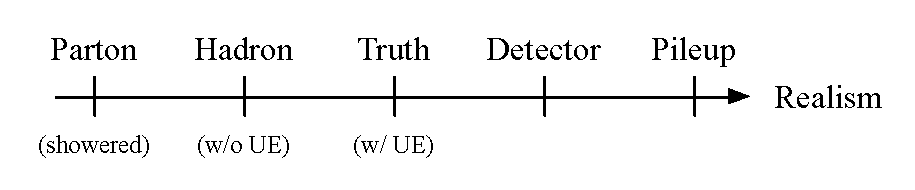
\includegraphics[width=0.75\columnwidth]{figures/realism_levels}
\end{center}
\caption{A summary of the different stages of physics considered in
  this study from idealized parton level events, to fully realistic
  events including detector simulation and pileup. This allows us to
  address robustness to physics at each stage. Detailed definitions of
  each stage, and the physics probe are given in the text. \gs{The
    ordering between detector and PU may have to be revised.} }
\label{fig:realism}
\end{figure}

We will approach robustness by moving from an idealized partonic description to a complete detector simulation including pileup; a``realistic" scenario representative of the LHC environment. This chain of realism is shown in \Fig{fig:realism}, which illustrates the following stages:
\begin{itemize}
\item Parton Level: We define the parton level result as the
  perturbative distribution for the active-active scattering (i.e. we
  do not include possible perturbative contributions to the underlying
  event). While this can be defined in an analytic calculation, it is
  more difficult in the context of parton shower Monte Carlos, as
  there is necessarily a cut-off that must be imposed between
  perturbative and non-perturbative physics. Only the complete result
  is physical, and intermediate results should be interpreted with
  care. Nevertheless, to have some measure of the impact of
  non-perturbative effects, we will define parton level as generated
  by a parton shower Monte Carlo with all hadronization effects turned
  off.
  %
  We will use multiple parton shower Monte Carlos with different
  hadronization models to ensure the robustness of our
  conclusions.\gs{We have only used Pythia so far, so I'd remove this
    sentence and add a footnote saying ``Ideally we would use multiple
    parton shower Monte Carlos with different hadronization models to
    ensure the robustness of our conclusions. This is left for future
    work.''}
\item Hadron Level: We define the hadron level result as that including hadronization in the shower, but not including any effects from the underlying event.
\item Truth Level: We define truth as the hadronized results including the underlying event as implemented in an event generator. Truth level therefore represents a complete hard scattering process in a hadron-hadron collider in isolation.
\item Detector Level: Detector level results are defined as truth level events passed through a detector simulation as implemented by TowerGrid. See \Sec{sec:det_model} for details of the detector simulation.
\item Pileup Level: In the final stage of realism we include pile-up
  by superimposing uncorrelated minimum bias events at detector
  level. These represent to the level that we can consider in this
  paper, realistic events as seen by the experiments at the
  LHC. \gs{We should briefly mention that we subtract pileup
    using... [fill this once we've agreed on what will be shown].}
\end{itemize}

Comparing the differences as we progress step by step through this sequence allows us to address at each stage the robustness to distinct physics issues, and we hope that our segmentation is sufficiently fine that we have a comprehensive view of robustness. In particular, the different steps in the chain allow us to study robustness to the following physics: 
\begin{itemize}
\item Parton$\to$ Hadron: Changes in the distribution from parton
  level to hadron level probe non-pertubative physics associated with
  hadronization. For many event shapes, hadronization corrections can
  be given a field theory definition in terms of a matrix element
  whose symmetry properties can be used to prove basic
  results. However, ultimately such corrections cannot be computed
  from first principles and must be included through models, such as
  those included in parton shower Monte Carlos, or through shape
  functions in analytic calculations
  \cite{Korchemsky:1999kt,Korchemsky:2000kp,Bosch:2004th,Hoang:2007vb,Ligeti:2008ac}
  \gs{Add references to the ``dispersive'' approach from
    hep-ph/9512336 and hep-ph/9504219}.  To have the best theoretical
  control and understanding of jet substructure observables, it is
  therefore desirable that their performance is robust to the effects
  of hadronization.
\item Hadron $\to$ Truth: Changes in the distribution from hadron level to truth level probe the impact of the underlying event, namely the physics associated with interactions of the colliding protons, and their remnants. Such contributions are in principle both perturbative and non-perturbative. They are poorly understood theoretically, and it is currently not known how to treat them systematically, or define them field theoretically. It has been found empirically that the effects of underlying event are well modeled by a shape function \cite{Stewart:2014nna}, although the theoretical justification for this is not clear.  The underlying event is implemented in Monte Carlo event generators using models which are tuned to data, and we take these models as our definition of the underlying event. Due to this lack of theoretical understanding, as well as the fact that radiation from the underlying event is typically not associated with the physics that we are interested in probing, it is desirable that jet substructure observables be robust to underlying event.
\item Truth $\to$ Detector: Since we are ultimately interested in using jet substructure in the experiments, the behavior of the detectors plays an essential role. The finite energy and spatial resolution of the detectors ultimately degrades the behavior of the observables. Furthermore, the detector response must be unfolded, and is therefore difficult to compute analytically, or to include to higher accuracy. Therefore, both for performance, and calculability it is desirable that jet substructure observables are robust to detector effects.
\item Detector $\to$ Pileup: Finally, due to the high-pile up environment of the LHC, significant soft radiation can contaminate the jet substructure observables of interest. Since this radiation is not correlated with the event of interest, it is not associated with the physics of interest, and therefore can only act to degrade the performance. Furthermore, it is difficult to model in an analytic calculation. While techniques exist to mitigate pile-up, as were reviewed in \Sec{sec:pu_tech}, it is desirable the substructure observables are as robust as possible to pile-up contamination.
\end{itemize}
We will classify the first two of these as sources of ``Theory" uncertainty, which will be discussed in \Sec{sec:np}, while the second two are classified as sources of ``Experimental" uncertainty, and will be discussed in \Sec{sec:exp}. This decomposition is of course somewhat arbitrary, as a coherent understanding involving the complete chain is required, however, it is chosen such that the ``Theory" issues cover an idealized hadronic collision in isolation. 

\begin{figure}
\begin{center}
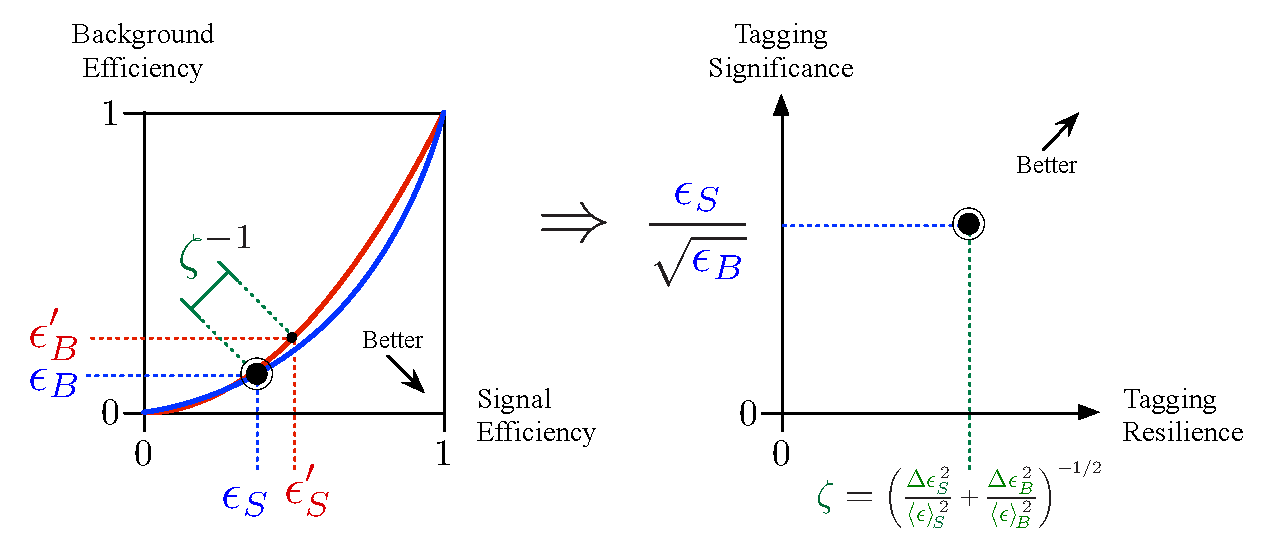
\includegraphics[width=1.0\columnwidth]{figures/roc_to_significance}
\end{center}
\caption{An illustration of the metric $\zeta$ used throughout the text to quantify robustness. In a) we illustrate graphically $\zeta$ as the change in ROC curve to a particular physics issue. In b), we illustrate the tagging resilience - tagging performance plane which we will use to graphically illustrate our results. A simultaneously robust and performant tagger lives in the upper right hand corner of this space. }
\label{fig:zeta_def}
\end{figure}

Having detailed the different stages we will consider, and the physics
that is included in each stage,  to compare the robustness to a
particular step in this chain for different observables, we must
introduce a metric. There is of course a large degree of arbitrariness
in the definition of the metric. For example, one could base the
metric on the shape of the signal or background distribution.
However, we are ultimately interested in the performance of the observable. We will therefore introduce a metric which is based on the modification of the ROC curve. \gs{The description below is not very clear how one gets all the
  $\epsilon_S$ and $\epsilon_B$. What about sth like the
  following: ``If we want to test the robustness a reference stage
  ``ref'' to another stage ``other'' (e.g., for hadronisation, the
  reference stage would be the hacron level and the other stage would
  be the parton level), one would first calculate the cut (on the jet
  shape) $v_{\text{cut}}$ and background efficiency
  $\epsilon_B^{\text{(ref)}}$ corresponding to a given, fixed, signal
  efficiency, $\epsilon_S^{\text{(ref)}}$ for the reference level.
  %
  Keeping the same cut on the shape one would then compute the signal
  and background efficiencies, $\epsilon_S^{\text{(other)}}$
  and$\epsilon_B^{\text{(other)}}$, for the other stage.
  %
  We then define the robustness $\zeta$ as
  %
  \begin{align}
    \zeta=\left(  \frac{\Delta \epsilon_S^2}{ (\epsilon_S^{\text{(ref)}})^2}  +\frac{\Delta \epsilon_B^2}{ (\epsilon_B^{\text{(ref)}})^2}  \right)^{-1/2}\,.
\end{align}
with
$\Delta
\epsilon_{S,B}=\epsilon_{S,B}^{\text{(other)}}-\epsilon_{S,B}^{\text{(ref)}}$.
  % 
  This approach gives an estimate of how much our signal and
  bbackground efficiencies have changed, for a given set of cuts, when
  going from one stage to another. }
We therefore define
\begin{align}
\zeta=\left(  \frac{\Delta \epsilon_S^2}{ \langle \epsilon \rangle_S^2}  +\frac{\Delta \epsilon_B^2}{ \langle \epsilon \rangle_B^2}  \right)^{-1/2}\,.
\end{align}
The meaning of $\zeta$ is illustrated in \Fig{fig:zeta_def}.
%
This metric does not detect, for example, a uniform shift in both the
signal and background distributions. \gs{I'd rephrase that sentence as
  ``Note that this metric would be non-zero for a uniform shift in both the
  signal and background distributions.''}
%
While this would of course be an undesirable feature of the
observable, since the physics associated with the signal distribution
and the background distribution are sufficiently different, we believe
such situations are perverse. We therefore believe that $\zeta$
provides a good metric for assessing the robustness of the
tagger. When presenting our results, we will characterize observables
in the plane of $\epsilon$ - $\zeta$, with better observables being in
the upper right corner. We find that this allows us to synthesize the
information about a large number of observables in a compact manner. A
similar metric and presentation style was used in \cite{Salam:2016yht}
to study robustness to non-perturbative effects. In addition to
showing plots of the $\epsilon$-$\zeta$ plane, we will, in particular
cases of interest, also show the modification of the distribution
itself to provide additional insight into the robustness of the
observable.


It is important to emphasize that it is impossible to completely
characterize an optimal observable, particularly as jet substructure
observables are being used for increasingly specific
purposes. However, we hope that issues that we have chosen to focus on
are representative of the issues that will be important for a broad
range of applications. Other aspects, such as stability as a function
of mass or $p_T$, which are important for certain applications, are
beyond the scope of the current project. \gs{We have studied the $p_t$
  dependence!} However, it would be interesting to investigate them
using similar techniques.


%%%%%%%%%%%%%%%%%%%%%%%%%%%%%%%%%%%%%%%
\section{Observable Definitions}\label{sec:obs_def}
%%%%%%%%%%%%%%%%%%%%%%%%%%%%%%%%%%%%%%%

In this section we summarize all the observable definitions that will be studied throughout this paper. This includes the definition of the jet substructure shape observables, the definition of the grooming procedures, and the definition of the pile-up subtraction schemes.  No new material is presented here, and we follow closely the presentation in the original references. Readers already familiar with the definitions can readily skip this section.



%%%%%%%%%%%%%%%%%%%%%%%%%%%%%%%%%%%%%%%
\subsection{Jet Shape Observables}\label{sec:shape_def}
%%%%%%%%%%%%%%%%%%%%%%%%%%%%%%%%%%%%%%%

The jet shape observables that we consider will be formed from ratios of either the energy correlation functions \cite{Larkoski:2013eya,Moult:2016cvt} or the $N$-subjettiness observables \cite{Thaler:2010tr,Thaler:2011gf}.  The $N$-subjettiness observables are defined as \cite{Stewart:2010tn,Thaler:2010tr,Thaler:2011gf}
\begin{equation}\label{eq:nsubdef}
\Nsub{N}{\beta} = \frac{1}{p_{TJ}}\sum_{1\leq i \leq n_J} p_{Ti}\min\left\{
R_{i1}^\beta,\dotsc,R_{iN}^\beta
\right\} \ .
\end{equation}
Here $p_{TJ}$ is the $p_T$ of the jet,  $p_{Ti}$ is the $p_T$ of particle $i$, and the sum is over all particles in the jet. The minimum is over the boost invariant angle
\begin{align}\label{eq:ptratio}  
R_{iJ}^2 = (\phi_i-\phi_J)^2+(y_i-y_J)^2\,,
\end{align}
between the particle $i$ and the axis $J$. For $N$-subjettiness there are $N$ axes.

Implicit in the definition of the $N$-subjettiness observable in
\Eq{eq:nsubdef} is the definition of the axes $n_i$. While their
placement is unambiguous (up to power corrections) in the limit of a
resolved substructure, an algorithmic definition is required to
determine their behavior in the unresolved limit.  Two main approaches
have been used for defining the axes. The first approach is to define
the $N$-subjettiness axes as the axes found using an exclusive jet
clustering algorithm, while the second is to minimize the sum in
\Eq{eq:nsubdef} over possible light-like axes $n_i$. In this paper we
use \ijm{check what Gregory did}\gs{``In this paper the axes are given
  bby the exclusive subjets obtained either by reclustering the jet
  with the $k_t$ algorithm~\cite{Catani:1993hr} and the
  Winner-takes-all recombination scheme~\cite{Larkoski:2014uqa} for
  $\beta=1$ $N$-subjettiness, or by reclustering the jet with the
  generalised $k_t$ algorithm~\cite{Cacciari:2011ma} with $p=1/2$, for
  $\beta=2$ $N$-subjettiness.''}




For two-prong tagging, the relevant observable is the ratio \cite{Thaler:2010tr}
\begin{align}
\Nsub{2,1}{\beta}\equiv \frac{\Nsub{2}{\beta}}{\Nsub{1}{\beta}}\,.
\end{align}
For a jet with a well resolved two-prong structure, we have $\Nsub{2,1}{\beta}\ll 1$, while for a jet without a well resolved substructure, we have $\Nsub{2,1}{\beta}\sim 1$.
This observable has been extensively used at the LHC. It has been calculated to LL accuracy \cite{Dasgupta:2015lxh}, and the effects of axes on the perturbative behavior have been studied at NLO \cite{Larkoski:2015uaa}.

The second class of observables that we will consider are based on the energy correlation functions \cite{Larkoski:2013eya}. Instead of correlating particles with axes, as is done for $N$-subjettiness, the idea of the energy correlation functions is to correlate $n$-tuples of particles.  In discussing the energy correlation function, it is convenient to work with dimensionless observables, written in terms of an energy fraction variable, $z$, and $R_{ij}$
\begin{align}\label{eq:ptratio}  
z_i\equiv\frac{p_{Ti}}{\sum_{j \in \text{jet}} p_{Tj}}\,, \qquad   R_{ij}^2 = (\phi_i-\phi_j)^2+(y_i-y_j)^2\,,
\end{align}
where $p_{Ti}$, $\phi_i$, and $y_i$ are the transverse momentum,
azimuthal angle, and rapidity of particle $i=1,\dots,n_J$ \gs{I've
  added ``$=1,\dots,n_J$'' so that the meaning of $n_J$ is clear in
  the equation bbelow}, respectively. 
%Tkachov \Ref{Tkachov:1995kk,Sveshnikov:1995vi,Cherzor:1997ak,Tkachov:1999py},
The general energy correlation function is defined as
\begin{equation}\label{eq:ecf_gen}
\ecfvar{v}{n}{\beta} = \sum_{1 \leq i_1 < i_2 < \dots < i_n \leq n_J} z_{i_1} z_{i_2} \dots z_{i_n} \prod_{m = 1}^{v} \min^{(m)}_{s < t \in \{i_1, i_2 , \dots, i_n \}} \left\{ R_{st}^{\beta} \right\},
\end{equation}
where $\min^{(m)}$ denotes the $m$-th smallest element in the list.  For a jet consisting of fewer than $n$ particles, $\ecfvarnobeta{v}{n}$ is defined to be zero.  More explicitly, the three arguments of the generalized energy correlation functions are as follows.
\begin{itemize}
\item The subscript $n$, appearing to the right of the observable, denotes the number of particles to be correlated.   
\item The subscript $v$, appearing to the left of the observable, denotes the number of pairwise angles entering the product.  By definition, we take $v \leq \binom{n}{2}$, and the minimum then isolates the product of the $v$ smallest pairwise angles.
\item The angular exponent $\beta>0$ can be used to adjust the weighting of the pairwise angles.
\end{itemize}




In this paper, we use the 2-point energy correlation function
\begin{align}\label{eq:explicit_twopointvar}
\ecfvar{1}{2}{\beta}&\equiv\ecf{2}{\beta}=\sum_{1\leq i<j\leq n_J} z_{i}z_{j} \, R_{ij}^\beta\ ,
\end{align}
as well as  the 3-point correlators
\begin{align}\label{eq:explicit_ecfvar}
\ecfvar{1}{3}{\beta}&=\sum_{1\leq i<j<k\leq n_J} z_{i}z_{j}z_{k} \min \left\{ R_{ij}^\beta\,,  R_{ik}^\beta\,, R_{jk}^\beta  \right\} \ , \nonumber \\
\ecfvar{2}{3}{\beta}&=\sum_{1\leq i<j<k\leq n_J} z_{i}z_{j}z_{k} \min \left\{R_{ij}^\beta R_{ik}^\beta\,, R_{ij}^\beta  R_{jk}^\beta\,,     R_{ik}^\beta R_{jk}^\beta    \right\}  \ , \nonumber \\
\ecf{3}{\beta}\equiv\ecfvar{3}{3}{\beta}&=\sum_{1\leq i<j<k\leq n_J} z_{i}z_{j}z_{k} \, R_{ij}^\beta R_{ik}^\beta R_{jk}^\beta \,.
\end{align}






 A number of powerful 2-prong discriminants have been formed from the energy correlation functions  \cite{Larkoski:2013eya,Larkoski:2014gra,Larkoski:2014zma,Moult:2016cvt}. Here we will focus on the observables
\begin{align}
 M_2^{(\beta)} = \frac{\ecfvar{1}{3}{\beta}}{\ecfvar{1}{2}{\beta}} \qquad  N_2^{(\beta)} = \frac{\ecfvar{2}{3}{\beta}}{(\ecfvar{1}{2}{\beta})^2}\,, \qquad  \Dobs{2}{\beta}=\frac{\ecf{3}{\beta}}{(\ecf{2}{\beta})^{3}}\,, 
\end{align}
each of which probes the correlations between particles within the jet in a slightly different manner. For a detailed discussion, see \cite{Moult:2016cvt}. The $N_2$ observable has been used by CMS, and the $D_2$ observable has been used by ATLAS. The $M_2$ observable is expected to be less performant, except in particular scenarios, but we include it to investigate the possibility that it might provide additional information. We will see that it also provides an example of a remarkably robust observable.


Beyond their discrimination power, these observables have nice theoretical properties.  First, since they can be written as a sum over particles in the jet without reference to external axes, they are automatically ``recoil-free'' \cite{Catani:1992jc,Dokshitzer:1998kz,Banfi:2004yd,Larkoski:2013eya,Larkoski:2014uqa}. Second, since they have well-defined behavior in various soft and collinear limits, they are amenable to resummed calculations;  in \Ref{Larkoski:2015kga}, $\Dobsnobeta{2}$ was calculated to next-to-leading-logarithmic (NLL) accuracy in $e^+e^-$ for both signal (boosted $Z$) and background (QCD) jets. 









%%%%%%%%%%%%%%%%%%%%%%%%%%%%%%%%%%%%%%%
\subsection{Grooming Techniques}\label{sec:groom_tech}
%%%%%%%%%%%%%%%%%%%%%%%%%%%%%%%%%%%%%%%

\gs{At the end,m we should make sure that our notations are uniform
  ``Soft Drop'', ``modified MassDrop Tagger'', ... I have fixed a few
  but we should do a more systematic check}

\gs{We should also stick to one of $p_t$ or $p_T$, and $p_f,J$
  v. $p_{t,\text{jet}}$.}

Groomers, which remove wide angle soft radiation and contamination from a jet, also play an important role in two-prong tagging. While a variety of different grooming approaches have been defined \cite{Butterworth:2008iy,Ellis:2009su,Ellis:2009me,Krohn:2009th,Dasgupta:2013via,Dasgupta:2013ihk}, we will focus on Soft Drop/mMDT, which are the most theoretically well understood, and which exhibit a number of nice theoretical properties, as well as trimming \cite{Krohn:2009th}, which is used by the ATLAS experiment. In this section, we review the definition of the Soft Drop/mMDT and trimming algorithms and their parameters.

Starting from a jet identified with an IRC safe jet algorithm (such as
anti-$k_t$ \cite{Cacciari:2008gp}), the Soft Drop algorithm is defined
using Cambridge/Aachen (C/A) reclustering
\cite{Dokshitzer:1997in,Wobisch:1998wt,Wobisch:2000dk}.  Specializing
to the case of $\beta=0$, where Soft Drop is equivalent to the
Modified MassDrop Tagger \cite{Dasgupta:2013ihk}, the algorithm
proceeds as follows: \gs{The description below is valid for any
  $\beta$. We can simply say ``It then proceeds as follows:'', and,
  below, say ``For $\beta=0$, one recover the Modified MassDrop
  Tagger~\cite{Dasgupta:2013ihk}.''}
\begin{enumerate}

\item Recluster the jet using the C/A clustering algorithm, producing an angular-ordered branching history for the jet.

\item Step through the branching history of the reclustered jet.  At each step, check the Soft Drop condition
\begin{align}\label{eq:sd_cut}
\frac{\min\left[ p_{Ti}, p_{Tj}  \right]}{p_{Ti}+p_{Tj}}> \zcut \left(   \frac{R_{ij}}{R}\right)^\beta \,.
\end{align}
Here, $\zcut$ is a parameter defining the scale below which soft radiation is removed.  If the soft drop condition is not satisfied, then the softer of the two branches is removed from the jet.  This process is then iterated on the harder branch.

\item The Soft Drop procedure terminates once the Soft Drop condition is satisfied.

\end{enumerate}
Given a jet that has been groomed with the soft drop procedure, we can
then measure any IRC safe observable on this jet and it will remain
IRC safe. The severity of the Soft Drop grooming can be adjusting by
tuning the parameters $\zcut$ and $\beta$. Larger values of $\zcut$
groom more radiation within the jet for a fixed value of $\beta$. On
the other hand, as $\beta$ is increased, the grooming becomes less
severe. Typically values of $\zcut$ are around $0.1$, while typical
values of $\beta$ are between $0$ and $2$.




Associated with the Soft Drop algorithm, we will also consider the observable $z_g$ as a means for performing polarimetry, in \Sec{sec:polar}. The $z_g$ observable is also referred to as the groomed momentum fraction, and is defined as
\begin{align}
z_g=\frac{\min\left[ p_{Ti}, p_{Tj}  \right]}{p_{Ti}+p_{Tj}}
\end{align}
for the first declustering that satisfies the Soft Drop criteria. This
observable probes the momentum sharing between the two prongs in the
jet. For $\beta=0$ \gs{This is true for any $\beta\ge 0$ (Maybe
  doubble-check w Jesse).}, this observable is Sudakov safe on QCD
jets.


In addition to Soft Drop/mMDT, we will also consider the trimming algorithm, since it is used by the ATLAS collaboration. Starting from a jet of radius $R$ identified with an IRC safe jet algorithm trimming is defined by the following procedure
\begin{enumerate}
\item Recluster the jet into subjets of radius $R_{\text{sub}}$.
\item Eliminate from the jet all particles in subjets that satisfy
  $p_t^{\text{subjet}} > z_{\text{cut}}p_{t,\text{jet}}$ \gs{I'd use
    $p_{t,\text{subjet}}$ sonce we're using subscripts everywhere.}.
\item The trimmed jet is then defined to consist of the remaining particles.
\end{enumerate}
Trimming has been experimentally shown to be a powerful grooming algorithm, and exhibits excellent mass resolution. However, trimming is known to suffer from non-global logarithms, and does not have a smooth spectrum as a function of the trimmed mass. The trimmed mass was analytically calculated in \cite{Dasgupta:2013ihk}. The trimming parameters used by ATLAS are $R_{\text{sub}}=0.2$,  $ \zcut=0.05$ and the $k_T$ algorithm to perform the reclustering.

%%%%%%%%%%%%%%%%%%%%%%%%%%%%%%%%%%%%%%%
\subsection{Pile-Up Removal}\label{sec:pu_tech}
%%%%%%%%%%%%%%%%%%%%%%%%%%%%%%%%%%%%%%%


Due to the high pile-up environment of the LHC, pileup mitigation techniques \cite{Cacciari:2007fd,Alon:2011xb,Soyez:2012hv,Tseng:2013dva,Krohn:2013lba,Cacciari:2014gra,Bertolini:2014bba} are also widely used, which eliminate soft radiation from the event. Since this radiation is uncorrelated with the underlying hard scattering, this can in principle be done, and a variety of techniques exist.  In this paper we will use Area Subtraction \cite{Cacciari:2007fd,Cacciari:2008gn} and SoftKiller \cite{Cacciari:2014gra} as representative of these techniques.

In the SoftKiller approach, the event is broken into patches, and we define
\begin{align}
\rho= \text{median} \left \{ \frac{p_{Ti}}{A_i}   \right \}\,.
\end{align}
SoftKiller then removes particles below a cutoff $p_t^{\text{cut}}$, chosen such that $\rho=0$. We have
\begin{align}
p_t^{\text{cut}}=\text{median} \{ p_{Ti}^{\text{max}} \}\,.
\end{align}
SoftKiller has been shown to provide good performance for removing pile-up contamination.

\ijm{elaborate a bit more}\gs{A few points (I'll try to come back to
  this part later): (i) maybe the 1st equation could go into the
  area--median description, (ii) do we want to give all the deteails
  of the area--median parameters we've used (I'd say yes), (iii) we
  should mention that SK is fast, (ic) wqe should add a reference to
  PUPPI as an alternative used by CMS.}

%%%%%%%%%%%%%%%%%%%%%%%%%%%%%%%%%%%%%%%
\section{Theory Approaches to Robust Ratio Observables}\label{sec:hybrid_ratio}
%%%%%%%%%%%%%%%%%%%%%%%%%%%%%%%%%%%%%%%









\gs{I'd drop the 1st sentence}
In this paper we are interested in the interplay between robustness
and performance for jet substructure observables.
%
The observables discussed in the previous section are designed to
distinguish boosted bosons from QCD jets using the detailed structure
of the radiation within the jets. From this perspective, it is then
immediately clear that there will be an interplay between performance
and robustness. By using a maximal amount of radiation within the jet,
the maximal information is available to distinguish the origin of the
jet.  However, an increased sensitivity to radiation also means an
increased sensitivity to contamination, both theoretically from
non-perturbative hadronization effects and underlying event, as well
as experimentally from pile-up. It also introduces sensitivity to the
experimental reconstruction of soft momenta in the event. On the other
hand, a tight grooming procedure, which removes radiation from within
the jet, is expected to reduce the ability to distinguish boosted
bosons from QCD jets.

In this section we introduce a classification of different tagging strategies which will be an organizing framework for our study of robustness and performance. This organization will be based on the idea of dichroic observables \cite{Salam:2016yht}, which are ratio observables constructed from combinations of groomed and ungroomed observables. In \Sec{sec:dichroic} we review the physics of the dichroic approach, for the example of the $\tau_{21}$ observable that has been studied in the literature. In \Sec{sec:dichroic_new} we generalize the dichroic construction to the energy correlation function based observables, and give definitions of dichroic $N_2$, $D_2$ and $M_2$ observables. This allows us to have multiple concrete examples of observables for each of our general tagging strategies. Then, in \Sec{sec:dichroic_sum} we present the complete set of tagging strategies that we will consider in this work, including the different parameters we will scan within each general class.


% It is therefore an interesting theoretical question how one can simultaneously optimize the discrimination power of the observable, while minimizing the effect of soft radiation. While in the most general sense, this is the question that we are trying to address in this paper, in the particular context of perturbative radiation, this question can be addressed using an understanding of the observables in the soft and collinear limits. 

%%%%%%%%%%%%%%%%%%%%%%%%%%%%%%%%%%%%%%%
\subsection{Review of the Dichroic Approach}\label{sec:dichroic}
%%%%%%%%%%%%%%%%%%%%%%%%%%%%%%%%%%%%%%%


In \cite{Salam:2016yht} the authors studied the $\tau_{21}$ ratio observable. They proposed that in addition to considering the standard $\tau_{21}$, and its groomed counterpart, one should also consider a mixed version, with a groomed denominator, and an ungroomed numerator. This observable was termed dichroic. Concretely, they considered the three observables
\begin{align}
 \tau_{21} =\frac{\tau_2}{\tau_1}  \,, \qquad \tau_{21}^{\text{groomed}} =\frac{\tau_2^\groomed}{\tau_1^\groomed}\,, \qquad \tau_{21}^{\text{dichroic}} =\frac{\tau_2}{\tau_1^\groomed}\,,
\end{align}
and they argued that the dichroic combination was optimal for performance, while also increasing the robustness to non-perturbative contamination. A detailed discussion of the dichroic approach, including perturbative calculations, was given in \cite{Salam:2016yht}. Here we briefly summarize the motivation for the observables, following closely the presentation in \cite{Salam:2016yht}. Readers interested in a more detailed discussion are refferred to \cite{Salam:2016yht}.

\begin{figure}[t!]
\begin{center}
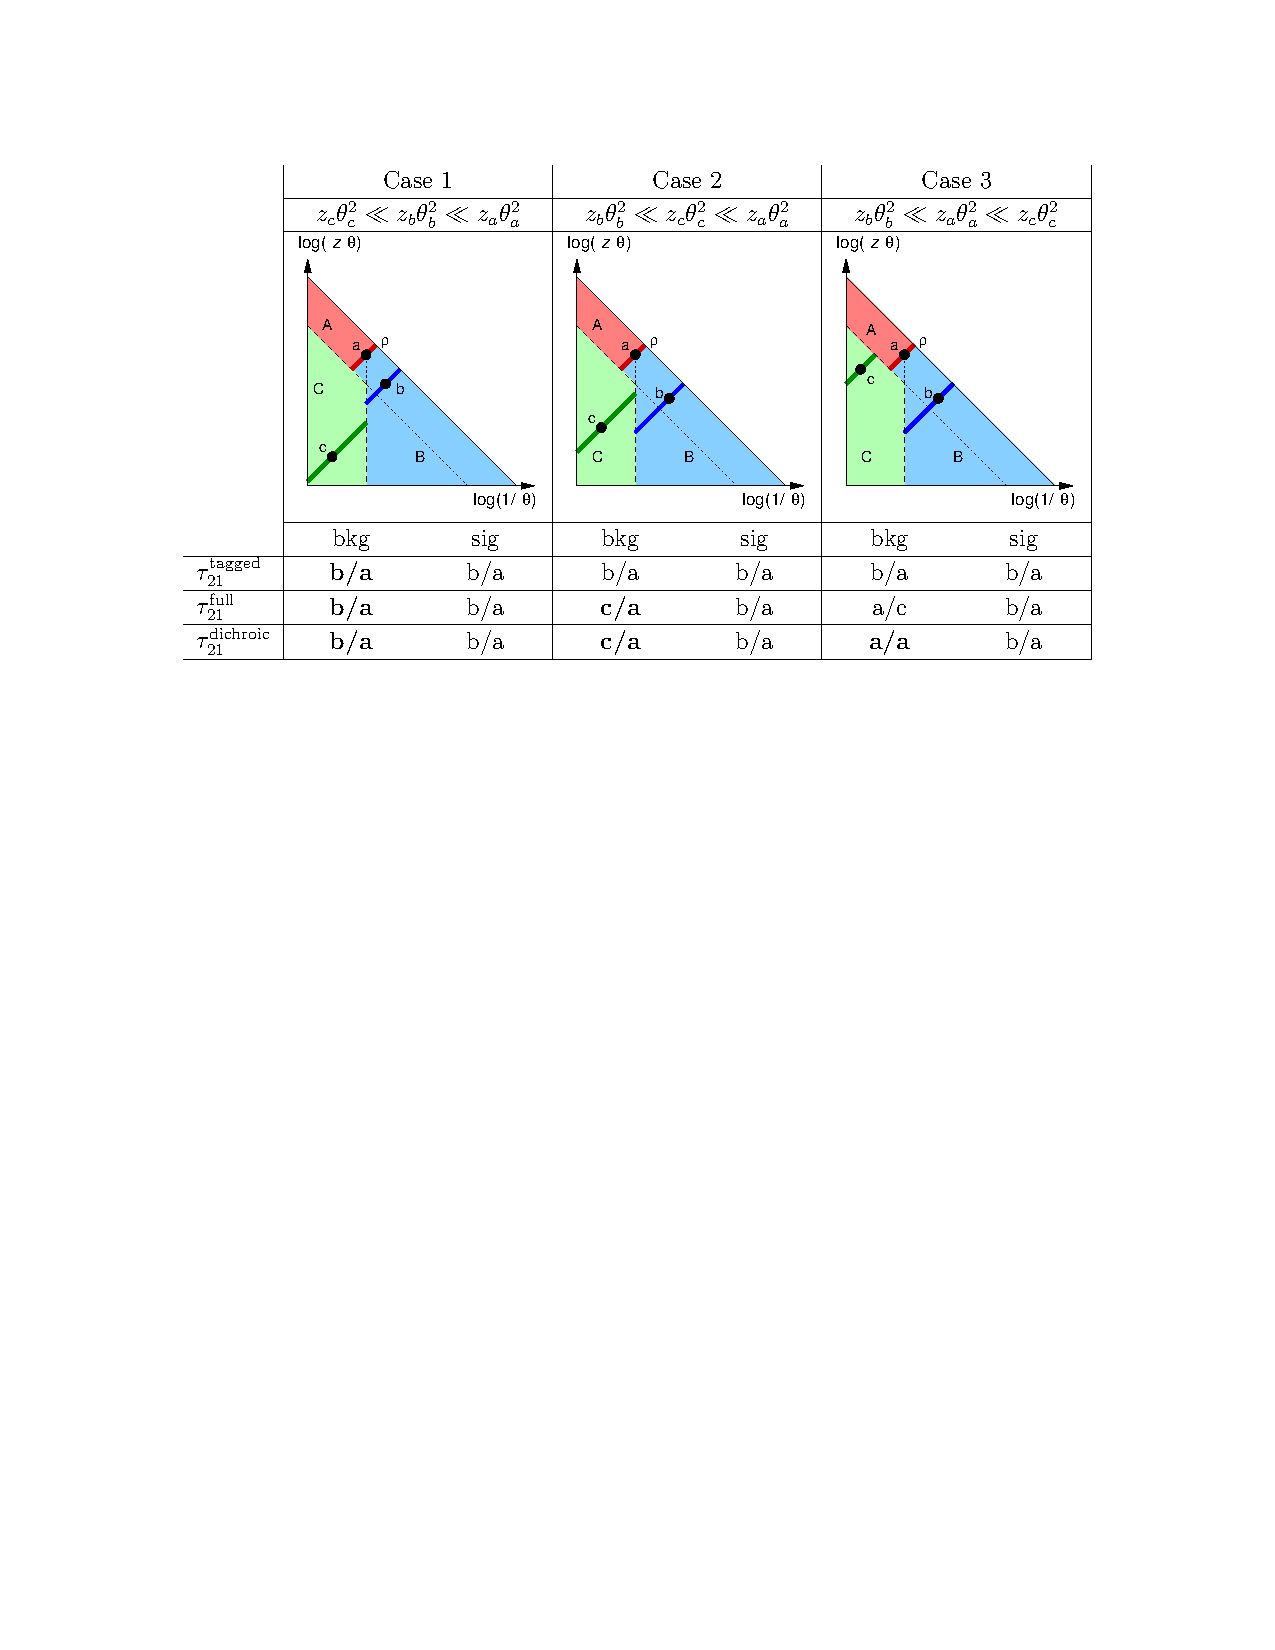
\includegraphics[width=0.75\columnwidth]{figures/dichroic_placeholder}
\end{center}
\caption{Lund diagrams depicting the three possible kinematic configurations for $\tau_{21}$ with a cut on the mMDT/soft dropped mass. A detailed explanation is provided in the text. Figure taken from \cite{Salam:2016yht}.}
\label{fig:dichroic}
\end{figure}




Using the Lund diagrams in \Fig{fig:dichroic}, we can give a simple argument for the optimal performance of the dichroic observables, by considering the behavior in each of the three regions
\begin{itemize}
\item Case 1: $z_c \theta_c^2 \ll z_b \theta_b^2 \ll z_a \theta_a^2$: All definitions of $\tau_{21}$ give the same result, and are therefore equivalent.
\item Case 2: $z_b\theta_b^2 \ll z_c \theta_c^2 \ll z_a \theta_a^2$: $\tau_{21}^\groomed=z_b \theta_b^2/z_a \theta_a^2 \ll  z_c \theta_c^2/z_a \theta_a^2=\tau_{21}=\tau_{21}^\dichroic$, showing that the groomed version performs suboptimally in this region of phase space.
\item Case 3: $z_b \theta_b^2 \ll z_a \theta_a^2 \ll z_c \theta_c^2$: $\tau_{21}^\dichroic=1$, and therefore $\tau_{21}^\dichroic \gg \tau_{21}$, $\tau_{21}^\dichroic \gg \tau_{21}^\groomed$. 
\end{itemize}
Since in all cases we have $\tau_{21}=z_b\theta_b^2/z_a\theta_a^2$ for
the signal, \gs{added the bit before} this shows that the dichroic
ratio is optimal. The identical argument can be reversed to show that
using a groomed numerator and an ungroomed denominator is not optimal.
\gs{If we have any for of space constraint, we can probably drop the
  discussion above and, optionally, replace it w a plot of the
  distributions (similar to Fig~7 in the dichroic paper), maybe
  including $\tau_{21}$ and $N_2$ or $D_2$.}

Since the dichroic ratio observable uses a partially groomed observable, it is also less sensitive to non-perturbative effects due to hadronization. It therefore represents an interesting new class of observable to consider in our study of robustness vs. performance. 







%%%%%%%%%%%%%%%%%%%%%%%%%%%%%%%%%%%%%%%
\subsection{New Dichroic Observables}\label{sec:dichroic_new}
%%%%%%%%%%%%%%%%%%%%%%%%%%%%%%%%%%%%%%%

The authors of \cite{Salam:2016yht} studied the dichroic $N$-subjettiness observable. It is however, straightforward to extend the definition to observables formed from the energy correlation functions. For $\tau_{21}$ it is immediately clear what the numerator and denominator of the observable are, however, this is initially less obvious for the energy correlation function based observables that have a more complicated structure. It can be shown that the correct prescription for the $M_2$, $N_2$ and $D_2$ observables is
%Recently it was proposed that 
%\begin{align}
%\mathcal{O}=\frac{\text{3-particle observable}}{\text{2-particle (mass) observable}}
%\end{align}
\begin{align}
M_2= \frac{ \ecfvarnobeta{1}{3}  }{\ecfnobeta{2}}\,, \qquad  M_2^{\text{groomed}}= \frac{ \ecfvarnobeta{1}{3}  }{\ecfnobeta{2}^\groomed}\,, \qquad  N_2^{\text{dichroic}}= \frac{\ecfvarnobeta{1}{3}  }{\ecfnobeta{2}^\groomed}\,, 
\end{align}
\begin{align}
N_2= \frac{\left( \ecfvarnobeta{2}{3} / \ecfnobeta{2} \right) }{\ecfnobeta{2}}\,, \qquad  N_2^{\text{groomed}}= \frac{\left( \ecfvarnobeta{2}{3} / \ecfnobeta{2} \right)^\groomed }{\ecfnobeta{2}^\groomed}\,, \qquad  N_2^{\text{dichroic}}= \frac{\left( \ecfvarnobeta{2}{3} / \ecfnobeta{2} \right) }{\ecfnobeta{2}^\groomed}\,, 
\end{align}
and
\begin{align}
D_2=\frac{\left( \ecfnobeta{3} / \ecfnobeta{2}^2 \right)}{ \ecfnobeta{2}}\,, \qquad D_2^{\text{groomed}}=\frac{\left( \ecfnobeta{3} / \ecfnobeta{2}^2 \right)^\groomed}{ \ecfnobeta{2}^\groomed}\,, \qquad D_2^{\text{dichroic}}=\frac{\left( \ecfnobeta{3} / \ecfnobeta{2}^2 \right)}{ \ecfnobeta{2}^\groomed}\,.
\end{align}
The above prescription is most easy to see for the $N_2$ observable. In the two-prong limit, the combination $ \ecfvarnobeta{2}{3} / \ecfnobeta{2} $ reduces to $\tau_2$, and therefore the dichroic $N_2$ ratio behaves similarly to the dichroic $\tau_{21}$ ratio.

%%%%%%%%%%%%%%%%%%%%%%%%%%%%%%%%%%%%%%%
\subsection{Summary of Tagging Strategies}\label{sec:dichroic_sum}
%%%%%%%%%%%%%%%%%%%%%%%%%%%%%%%%%%%%%%%

To be able to draw the most general conclusions regarding robustness and performance, we do not want to focus on the study of particular observables, but rather classes of observables, from which the known examples, such as those used by ATLAS or CMS are specific examples. In this way we can draw general conclusions about tagging strategies that should be robust to changes in specific application.

%%%
\begin{table}
\begin{center}
\begin{tabular}{| l | c | c |c |c|c|c |c|r| }
  \hline                       
  Observable &  Numerator & Denominator \\
  \hline
  $M_2$ &   $\ecfvarnobeta{1}{3}$ & $ \ecfnobeta{2}$ \\
  $N_2$ &   $\ecfvarnobeta{2}{3} / \ecfnobeta{2} $ & $ \ecfnobeta{2}$ \\
  $D_2$ &   $\ecfnobeta{3} / \ecfnobeta{2}^2 $ & $ \ecfnobeta{2}$ \\
  $\tau_{21}$ &   $\tau_2$ & $\tau_1$ \\
  \hline  
\end{tabular}
\end{center}
\caption{
Definitions of the numerators and denominators for the different jet
substructure observables. \gs{Added $M_2$; added an horizontal line in this table
  and the ones below}
}
\label{tab:dn}
\end{table}


The tagging strategies we consider can be put into the general form of a (groomed) mass cut followed by a cut on a two-prong tagging observable, which takes the form
\begin{align}
\mathcal{O}=\frac{\text{3-particle observable}}{\text{2-particle (mass) observable}} \equiv \frac{n}{d}\,.
\end{align}
The explicit numerators and denominators for the different observables are summarized in \Tab{tab:dn}. In general we want to have
\begin{align}
m \leq d \leq n\,,
\end{align}
for a performant observable.
As our organizing principle for classes of  jet substructure taggers, we will use the type of grooming applied to the initial mass cut, and the type of grooming applied to the numerator and denominator of the two-prong observable.


%%%
\begin{table}[t!]
\begin{center}
\begin{tabular}{| l | c | c |c |c|c|c |c|r| }
  \hline                       
  Notation: $m \otimes \frac{n}{d}$ & Mass & Numerator & Denominator\\
  \hline
  $p \otimes \frac{p}{p}$ & plain  &  plain & plain \\
  $l \otimes \frac{p}{p}$ & loose  &  plain & plain \\
  $l \otimes \frac{l}{p}$ & loose  &  loose & plain \\
  $t \otimes \frac{p}{p}$ & tight  &  plain & plain \\
  $t \otimes \frac{l}{p}$ & tight  &  loose & plain \\
  $t \otimes \frac{l}{l}$ & tight  &  loose & loose \\
  $t \otimes \frac{t}{p}$ & tight  &  tight & plain \\
  $t \otimes \frac{t}{l}$ & tight  &  tight & loose \\
  $t \otimes \frac{t}{t}$ & tight  &  tight & tight \\
  $\text{trim}$ & trim &  trim & trim \\
  \hline  
\end{tabular}
\end{center}
\caption{
A summary of the different tagging strategies considered, including the notation, and the degree of grooming for the mass, and numerator and denominator of the shape observable. For simplicity, we have suppressed the jet radius, $R$. The definitions of plain, loose, tight and trim are given in the text.
}
\label{tab:tag_summary}
\end{table}


\begin{itemize}
\item Plain: no grooming applied
\item loose: Soft Drop with $\zcut=0.05$, $\beta=2$ \gs{add ``Soft Drop''}
\item tight: mMDT with $\zcut=0.1$ \gs{added mMDT and removed $\beta=0$}
\item Trim: trimming with $R_{\text{sub}}=0.2$,  $ \zcut=0.05$ and the $k_T$ algorithm to perform the reclustering, as used by ATLAS.
\end{itemize}
We will use the notation 
\begin{align}
m \otimes \frac{n}{d} \otimes R
\end{align}
to denote the grooming applied to a particular observable. Here $R$ denotes the jet radius. The complete set of configurations that we will consider is given in \Tab{tab:tag_summary}. These constitute generic grooming strategies, and will be studied for each of $N_2$, $D_2$, and $\tau_{21}$. They include the dichroic ratios, as well as the current ATLAS and CMS approaches as specific examples.  This will allow us to draw powerful and general conclusions about the performance and robustness of jet substructure taggers.






While our general approach is based on studying the different classes of grooming strategies in \Tab{tab:tag_summary}, for each of these different classes of strategies, we will scan different parameters. In particular, we will scan the jet radius, jet shape, jet shape angular exponent, and jet $p_T$. The values scanned are summarized in \Tab{tab:params}. This allows us to understand if the conclusions drawn are associated with specific observables within a given strategy, as well as to optimize over these parameters. Due to the large number of physics and detector parameters that are varied in our study, only a subset of plots can be found in the paper. Additional plots of interest can be found in \App{app:more_plot}.



%%%
\begin{table}
\begin{center}
\begin{tabular}{| l | c | c |c |c|c|c |c|r| }
  \hline                       
  Parameter &  Values Scanned \\
  \hline
  Jet Radius $R$ &   $0.6$, $0.8$, $1.0$, $1.2$ \gs{We only did 0.8 and 1} \\
  Jet Shape  &   $D_2$, $N_2$, $M_2$, $\tau_{21}$  \\
  Jet Shape Angular Exponent $\beta$ &   $1$, $2$ \\
  Jet $p_T$ &   $500$ GeV, $1000$ GeV, $2000$ GeV  \\
  \hline  
\end{tabular}
\end{center}
\caption{
Jet shapes and parameters scanned for each of the different strategies proposed in \Tab{tab:tag_summary}.
}
\label{tab:params}
\end{table}












%%%%%%%%%%%%%%%%%%%%%%%%%%%%%%%%%%%%%%%
\section{Samples and Detector Models}\label{sec:samples}
%%%%%%%%%%%%%%%%%%%%%%%%%%%%%%%%%%%%%%%


In this section we describe in detail the samples that we will use throughout the papers. \Sec{sec:samples_sub} discusses the event generation, and \Sec{sec:det_model} discusses the details of the detector modelling. 

%%%%%%%%%%%%%%%%%%%%%%%%%%%%%%%%%%%%%%%
\subsection{Samples}\label{sec:samples_sub}
%%%%%%%%%%%%%%%%%%%%%%%%%%%%%%%%%%%%%%%

\ijm{need to make sure that this is correct}

For background samples, we generated $pp\to$ dijets in both \pythia{8.226} \cite{Sjostrand:2006za,Sjostrand:2007gs} with tune $4$C,   and \textsc{Herwig} 7~\cite{Bahr:2008pv,Bellm:2015jjp}. Samples were generated with hadronization off, with hadronization on, but underlying event off, and with hadronization and underlying event on.





Regarding the polarised $W$ samples, we consider a $gg$ produced resonance, $X$, that decays to a pair of polarized $W$ bosons. This kind of resonances decaying to longitudinally polarised $W$s appear in warped extra-dimensional models, where the SM fields propagate in the bulk. On the other hand, models with graviton-like tensor with minimal couplings yields only transversely polarized $W$ bosons. They were produced with the \textsc{JHUGEN} 3.1.8~\cite{Gao:2010qx,Bolognesi:2012mm} generator, interfaced with \textsc{PYTHIA} 8 \cite{Sjostrand:2007gs} for parton showering including the effect of hard gluon radiation. Additional samples interfaced with \textsc{Herwig} 7~\cite{Bahr:2008pv,Bellm:2015jjp} were also used to study shower differences. A resonance width of 1\% was chosen. Table~\ref{table:polarisedSamples} shows the coupling values used to generate the polarised $W$ samples (see also Ref.~\cite{Gao:2010qx} for more information). 

\begin{table}[ht]
\centering
\begin{tabular}{|c|c|c|c|}
\hline
Model	&Production couplings	&Decay couplings	&Decay helicity amplitudes 	\\
\hline
$2_b^+$	& $g_1=1$		& $g_5=1$		& $f_{00}=0.98$			\\
$2_m^+$	& $g_1=1$		& $g_1=g_5=1$		& $f_{00}=0.08,f_{+-}=f_{-+}=0.46$\\	
\hline
\end{tabular}
\caption{\gs{Add caption. (I've changed the layout so it is coherent w
  the previous tables)}}
\label{table:polarisedSamples}
\end{table}

To include pile-up we \ijm{fill in}


%%%%%%%%%%%%%%%%%%%%%%%%%%%%%%%%%%%%%%%
\subsection{Detector Models}\label{sec:det_model}
%%%%%%%%%%%%%%%%%%%%%%%%%%%%%%%%%%%%%%%

\ijm{Description of TowerGrid, and the differeces between the ATLAS and CMS detectors. }
\ijm{I have nothing here.}\gs{It would be great (best?) if Peter could
  write a little sth here} 

\begin{figure}
\begin{center}
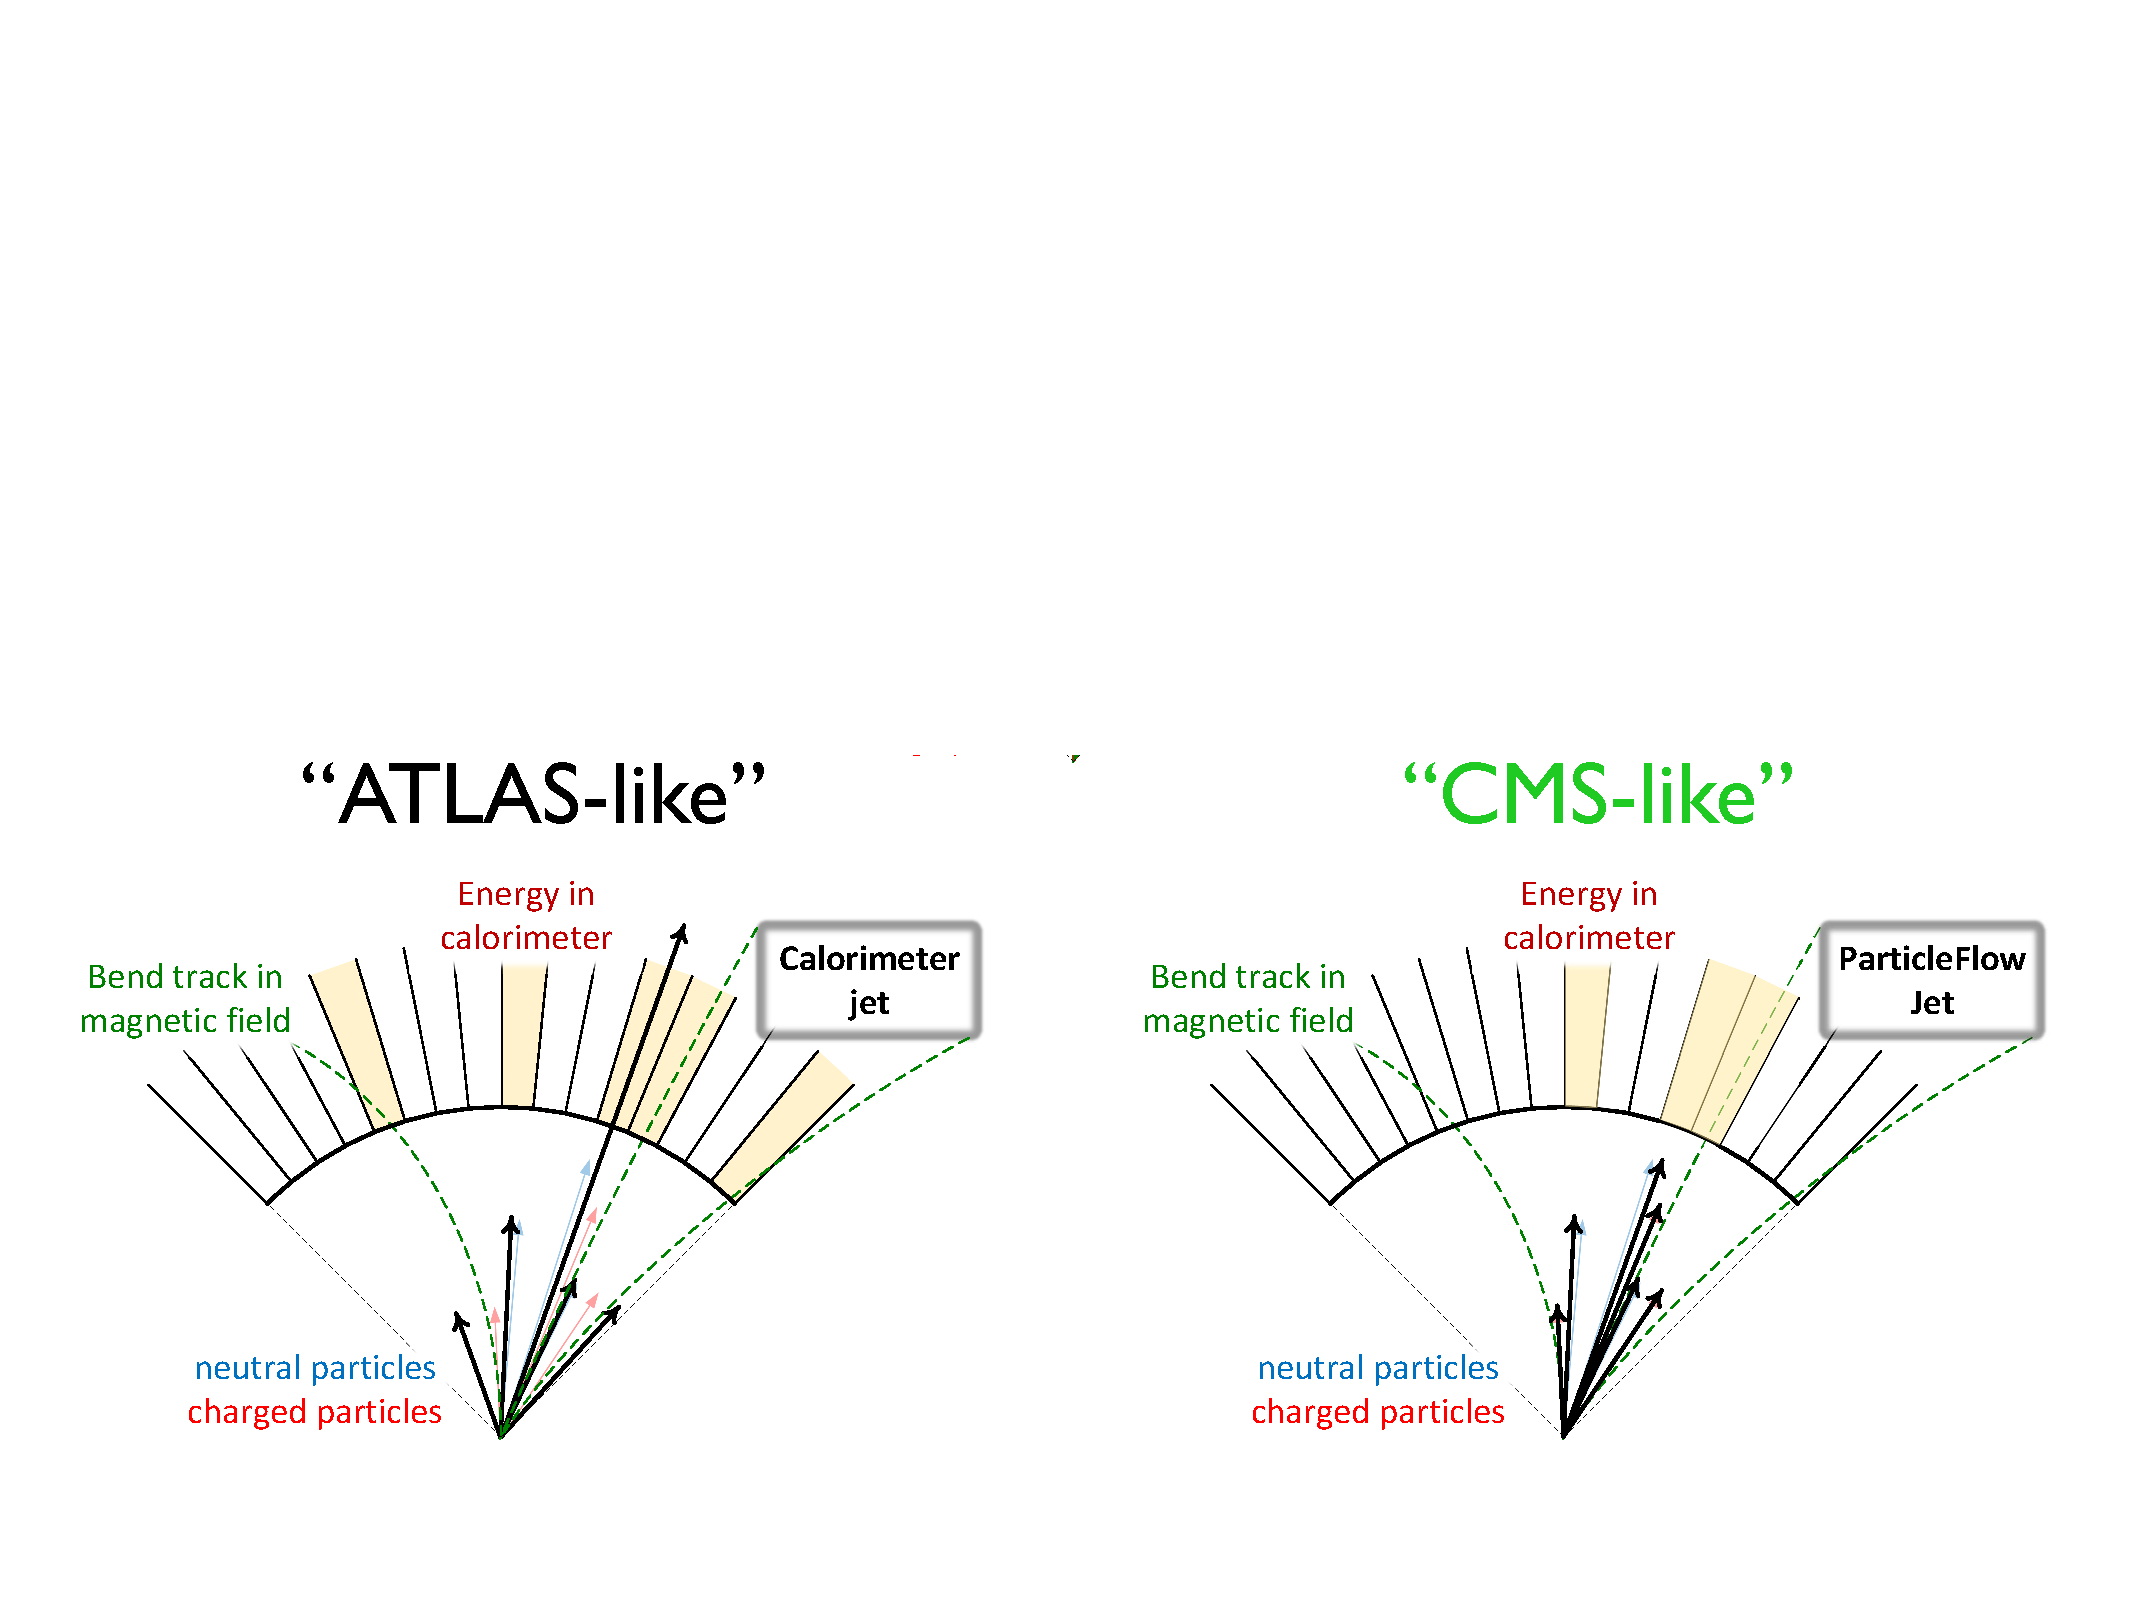
\includegraphics[width=1.0\columnwidth]{figures/CMS_vs_ATLAS_detector}
\end{center}
\caption{An illustration of the basic features of the CMS and ATLAS detectors.}
\end{figure}




%%%%%%%%%%%%%%%%%%%%%%%%%%%%%%%%%%%%%%%
\section{Signal Robustness}\label{sec:polar}
%%%%%%%%%%%%%%%%%%%%%%%%%%%%%%%%%%%%%%%

\gs{I think this section needs a bit of work. Quite a few things can
  be simplified/shortened. For example, I'd remove Figure 5. I agree
  that there are probably 2 questions here: (i) is our $W-QCD$
  separation robust against the polarisation of the $W$? (ii) can we
  discriminate longitudinal and transvers $W$'s?. For (i), we could
  show one or two distributions and a $\zeta-\epsilon$ plot (now sure
  which one, I'll probably know once we've decided what to show for
  the plots further down). For (ii), I have done $z_g$ plots and ROC
  curves and updated Figs 9 and 10 (which we could probably merge as a
  single fig). I'm also wondering if we should not move this down
  (i.e. first descrtibe the theory robustness which is what we've
  highlighted in Section 2.)}


The focus of this paper is on the robustness of jet substructure
observables for two-prong tagging. As has been discussed, for
background QCD jets one is interested in robustness to additional QCD
contamination and detector effects. On the other hand, for signal
jets, which have a well defined substructure, the behavior of taggers
is naturally robust to contamination from low energy QCD radiation
\gs{Is that clear/true? E.g. there is a $\Delta\epsilon_S/\epsilon_S$
  in our definition of $\zeta$.}. However, they can be sensitive to the
specific nature of the decaying electroweak scale particle. Assuming
that this is a color singlet decaying to quarks, it is completely
characterized by its spin structure. Jet substructure techniques have
mainly been applied to identify boosted $W/Z$ bosons from new BSM
resonances, or to look directly for new light particles decaying
hadronically \cite{CMS-PAS-EXO-17-001}. In both cases, one would like
to be able to perform the tagging independent of any assumptions about
the details of the spin structure. Additionally, it is an interesting
question whether jet substructure measurements can be used to
reconstruct the polarization of the object. It is our perspective that
ideally we would like to be able to separate these two aspects, namely
tagging two prong objects in a way that is robust to assumptions about
the details of the spin structure, as well as having tools to identify
the polarization. In this section we address two main issues, namely
the robustness of the standard jet substructure observables to the
polarization of the signals, and the ability to tag polarizations
using jet substructure observables measured on the hadronic decay
products.



%%%%%%%%%%%%%%%%%%%%%%%%%%%%%%%%%%%%%%%
\subsection{Physics of Polarization Dependence}\label{sec:polar_physics}
%%%%%%%%%%%%%%%%%%%%%%%%%%%%%%%%%%%%%%%

Before beginning \ijm{review basic kinematics and give expressions for the distributions before and after boost}

This is illustrated in \Fig{fig:spin_boost}



All of our taggers consist of two conceptually distinct components, which will be effected in different ways by the polarization. In particular, for all of our taggers we begin by making a cut on the (groomed) mass, followed by a cut on a particular jet shape which is sensitive to the two prong structure.

These two steps are associated with very different physics, particularly for a $W\to q\bar q$ decay, which has two well resolved prongs. A schematic of the QCD radiation surrounding this two prong structure is shown in \Fig{fig:spin_boost_dressed}. It consists of two collimated sprays of radiation, which are proxies for the $q$ and $\bar q$, along with radiation emitted from the dipole. If working as intended, the soft drop groomed should terminate when it de-clusters into two subjets corresponds to the jets around the two quarks. However, if there are a large fraction of decays where the momentum sharing between the two is hierarchical, then the soft drop groomer can groom away one of the subjets. In this case, the jet will fail to pass the soft drop mass criteria. This introduces a sensitivity on the polarization into the tagging procedure. On the other hand, the $2$-prong tagging observables that we consider are all formed as ratios of an observable which is sensitive to radiation from the prongs, divided by a mass type observable. This makes these observables largely insensitive to the polarization.

%%%%%%%%%%%%%%%%%%%%%%%%%%%%%%%%%%%%%%%
\subsection{Robustness to Polarization}\label{sec:polar_robust}
%%%%%%%%%%%%%%%%%%%%%%%%%%%%%%%%%%%%%%%


Before addressing the possibility of tagging particular polarizations, we begin in this section by studying the sensitivity of the different taggers to polarization. To do this, we will consider samples of hadronically decaying $W$s, which are either purely transversely polarized, purely longitudinally polarized, or have the Standard Model fraction (mostly transverse). The details of the sample generation were discussed in \Sec{sec:samples}.






\begin{figure}
\begin{center}
\subfloat[]{\label{fig:spin_boost_bare}
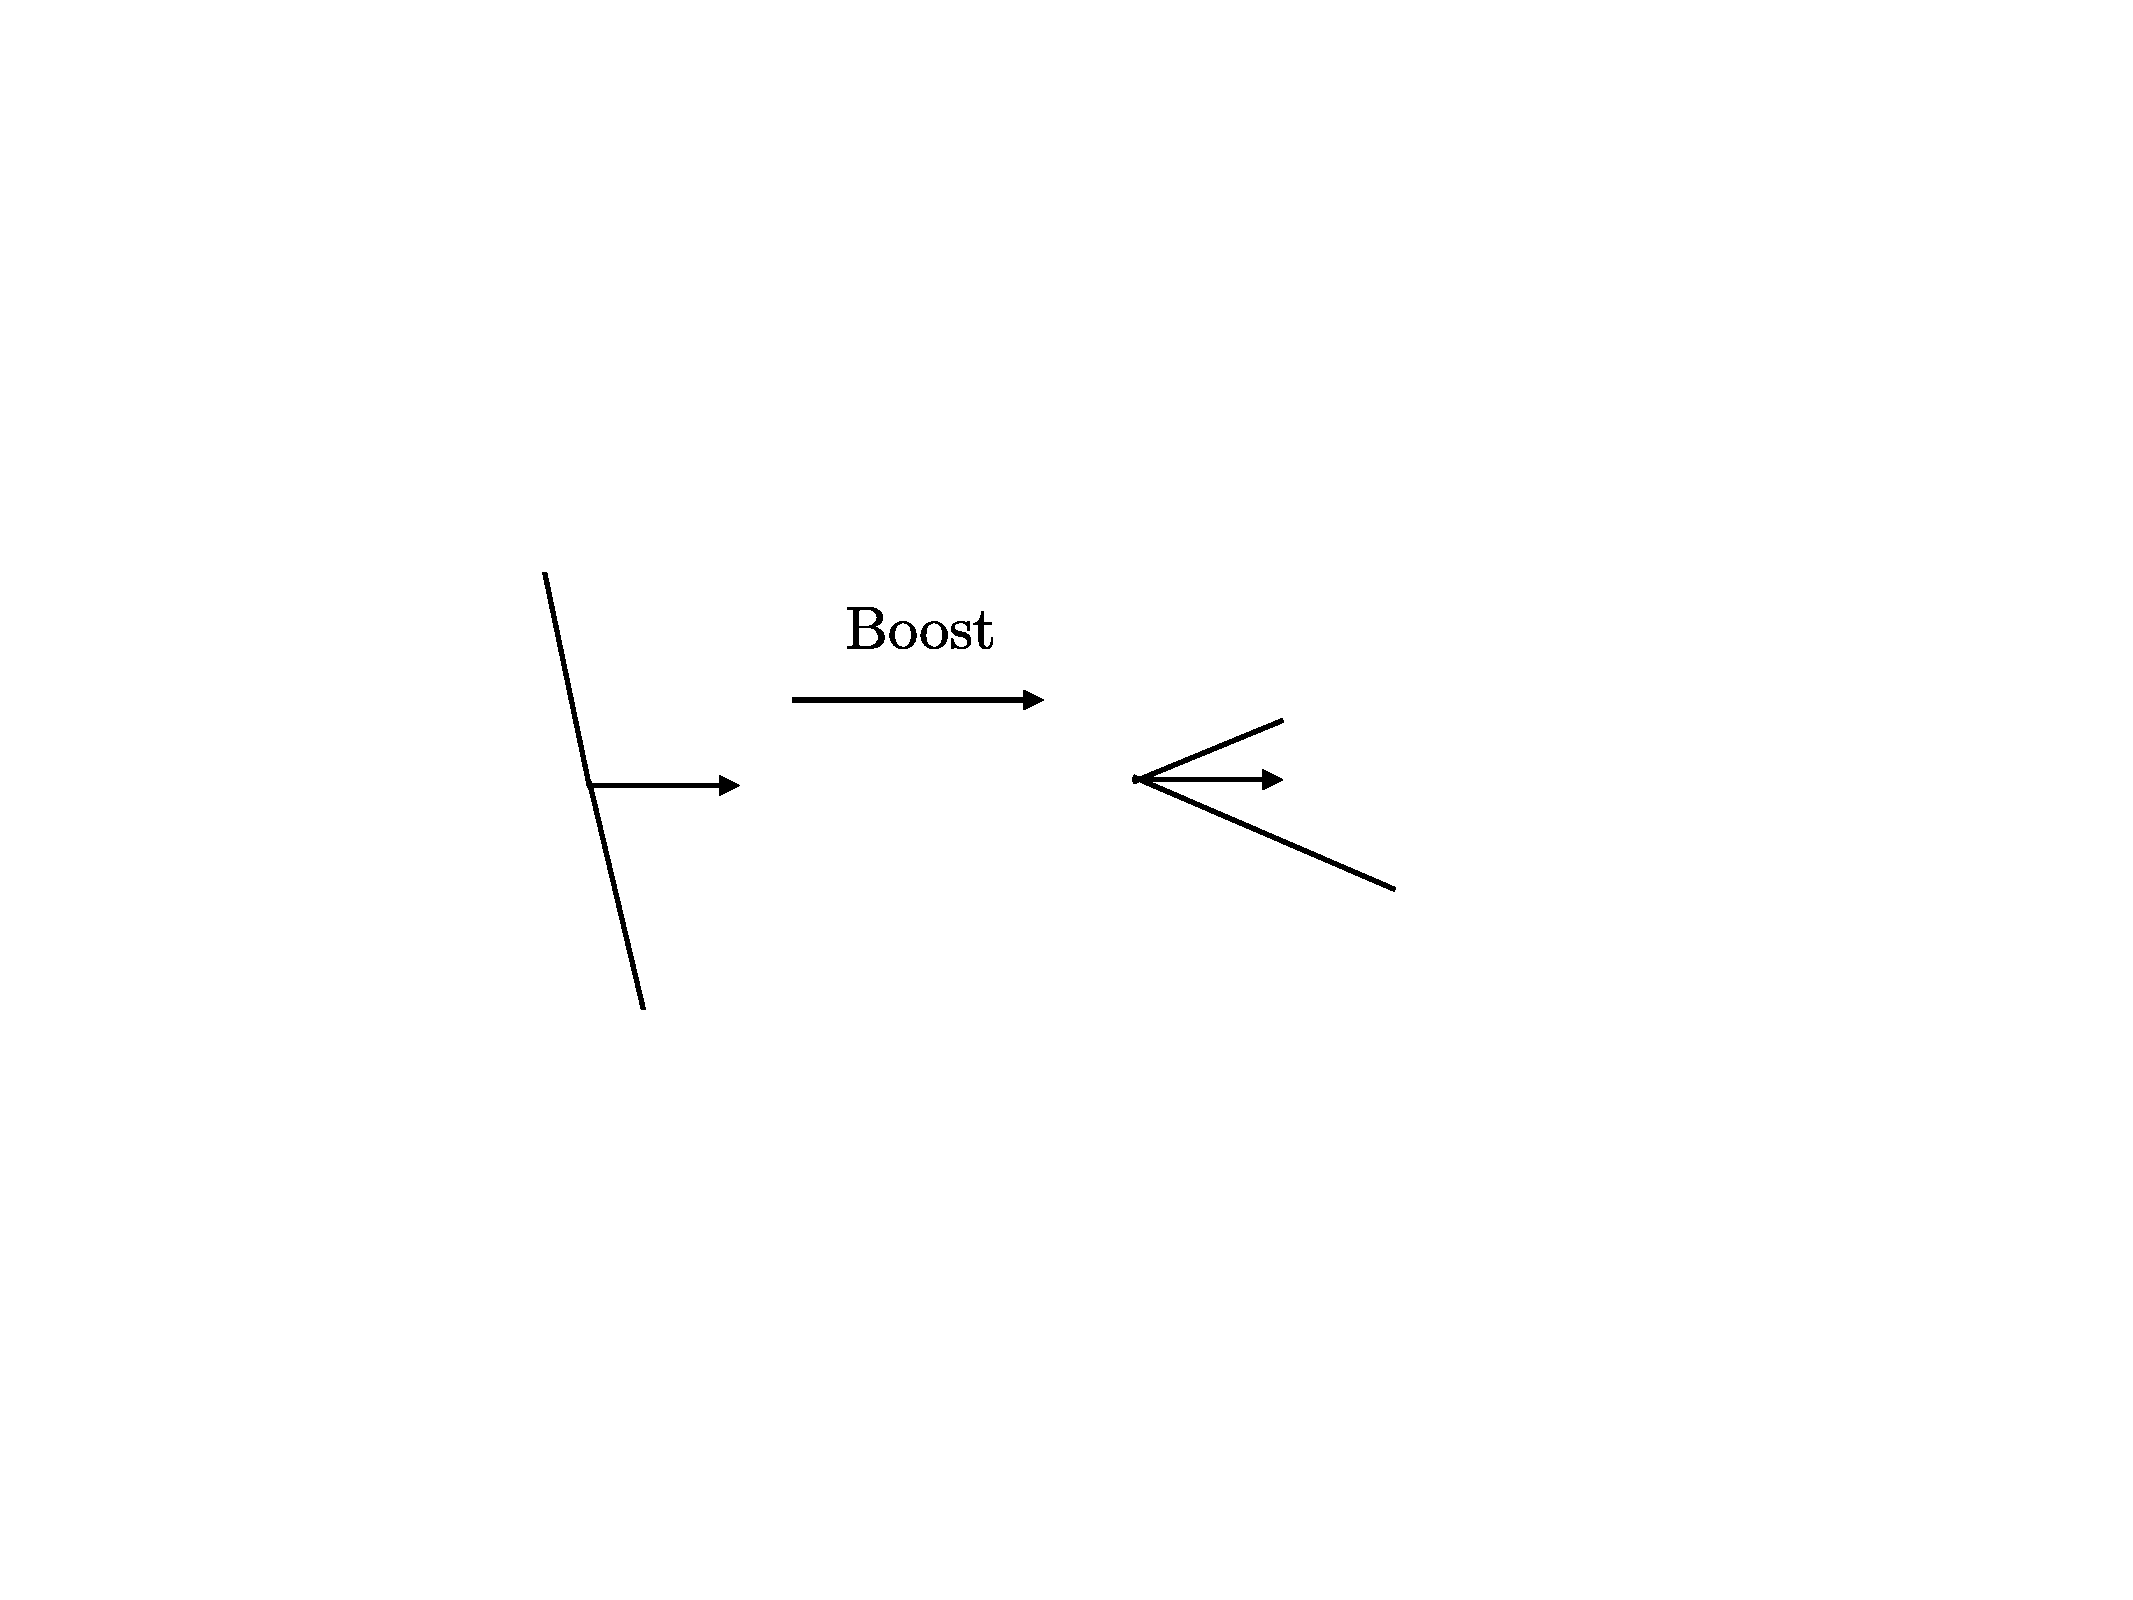
\includegraphics[width=7cm]{figures/spin_placeholder}    
}\qquad
\subfloat[]{\label{fig:spin_boost_dressed}
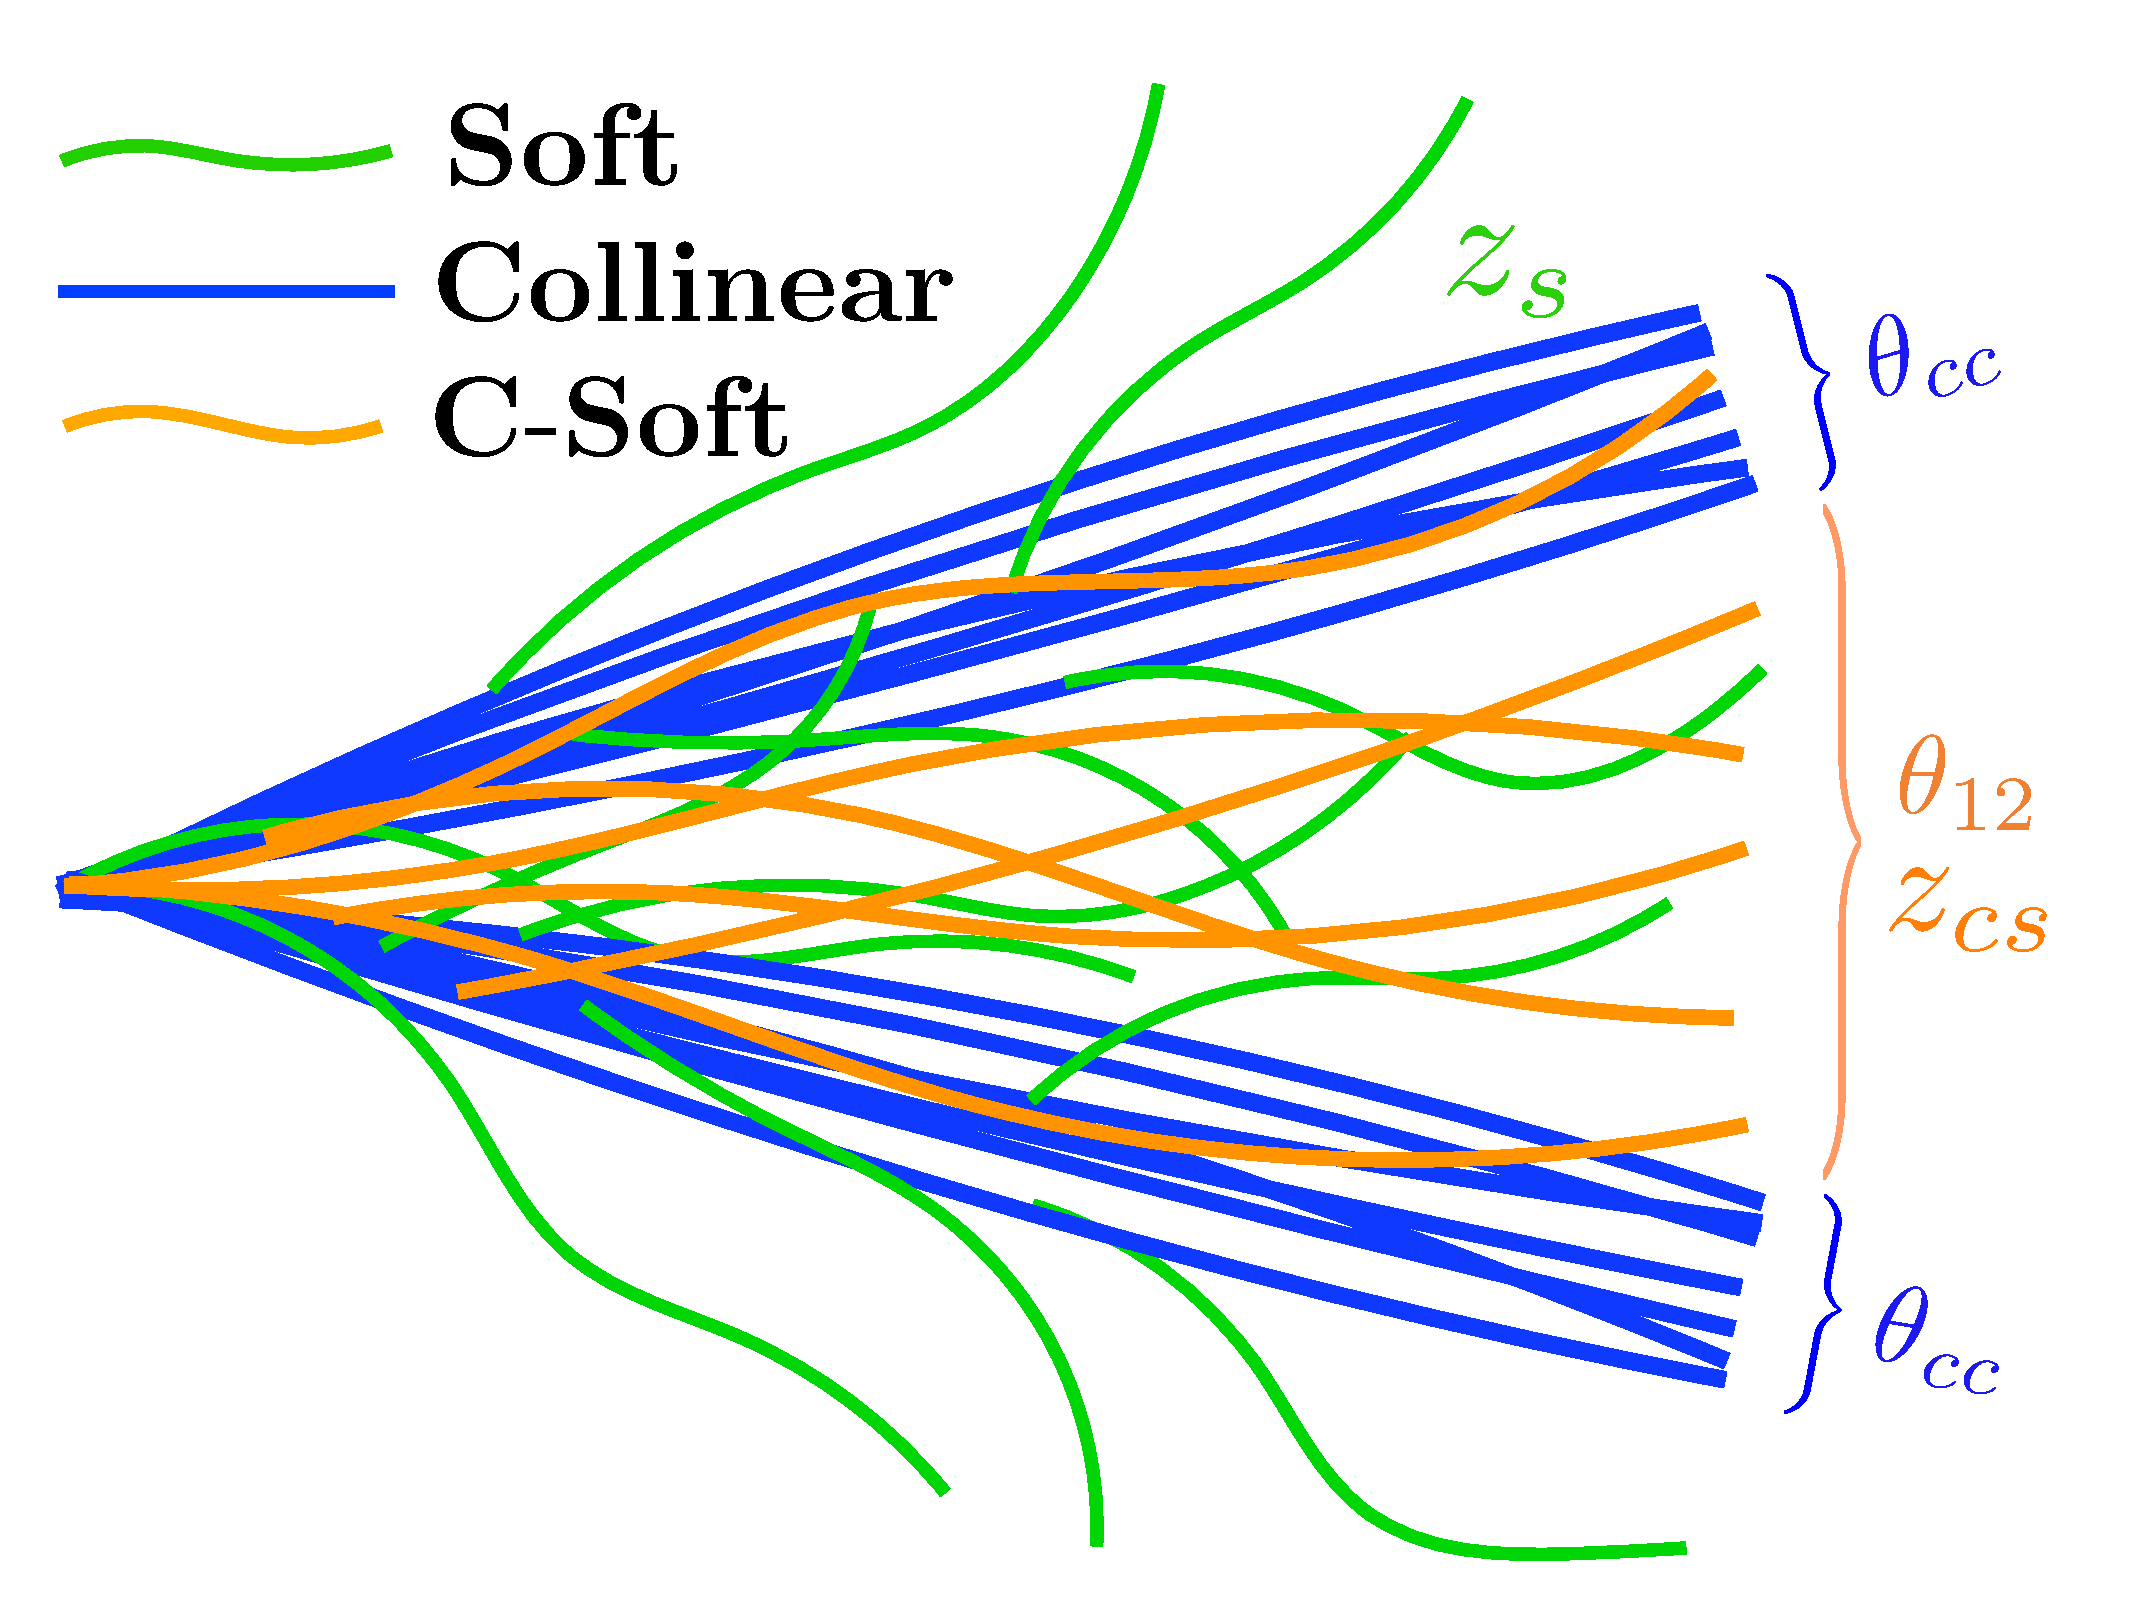
\includegraphics[width=5cm]{figures/NINJA}
}
\end{center}
\caption{a) An illustration (placeholder) of the origin of the polarization dependence for a boosted $W$ decay. Different polarizations give rise to different angular distributions in the $W$ boson rest frame, which, when boosted, give rise to different distributions for the momentum sharing. (placeholder) b) The decaying $W$ is dressed by radiation, however, the subjets act as proxies for the quarks in the decay and their properties carry most of the polarization information of the decay.
}
\label{fig:spin_boost}
\end{figure}






\ijm{if goal is just to tag, i.e. look for a two prong substructure, then we want to be ambivalent to the polarization. or else it needs to be included as a model assumption}

\ijm{difference between polarization for the actual shape, and the acceptenace for the jet mass cut}


\begin{figure}
\begin{center}
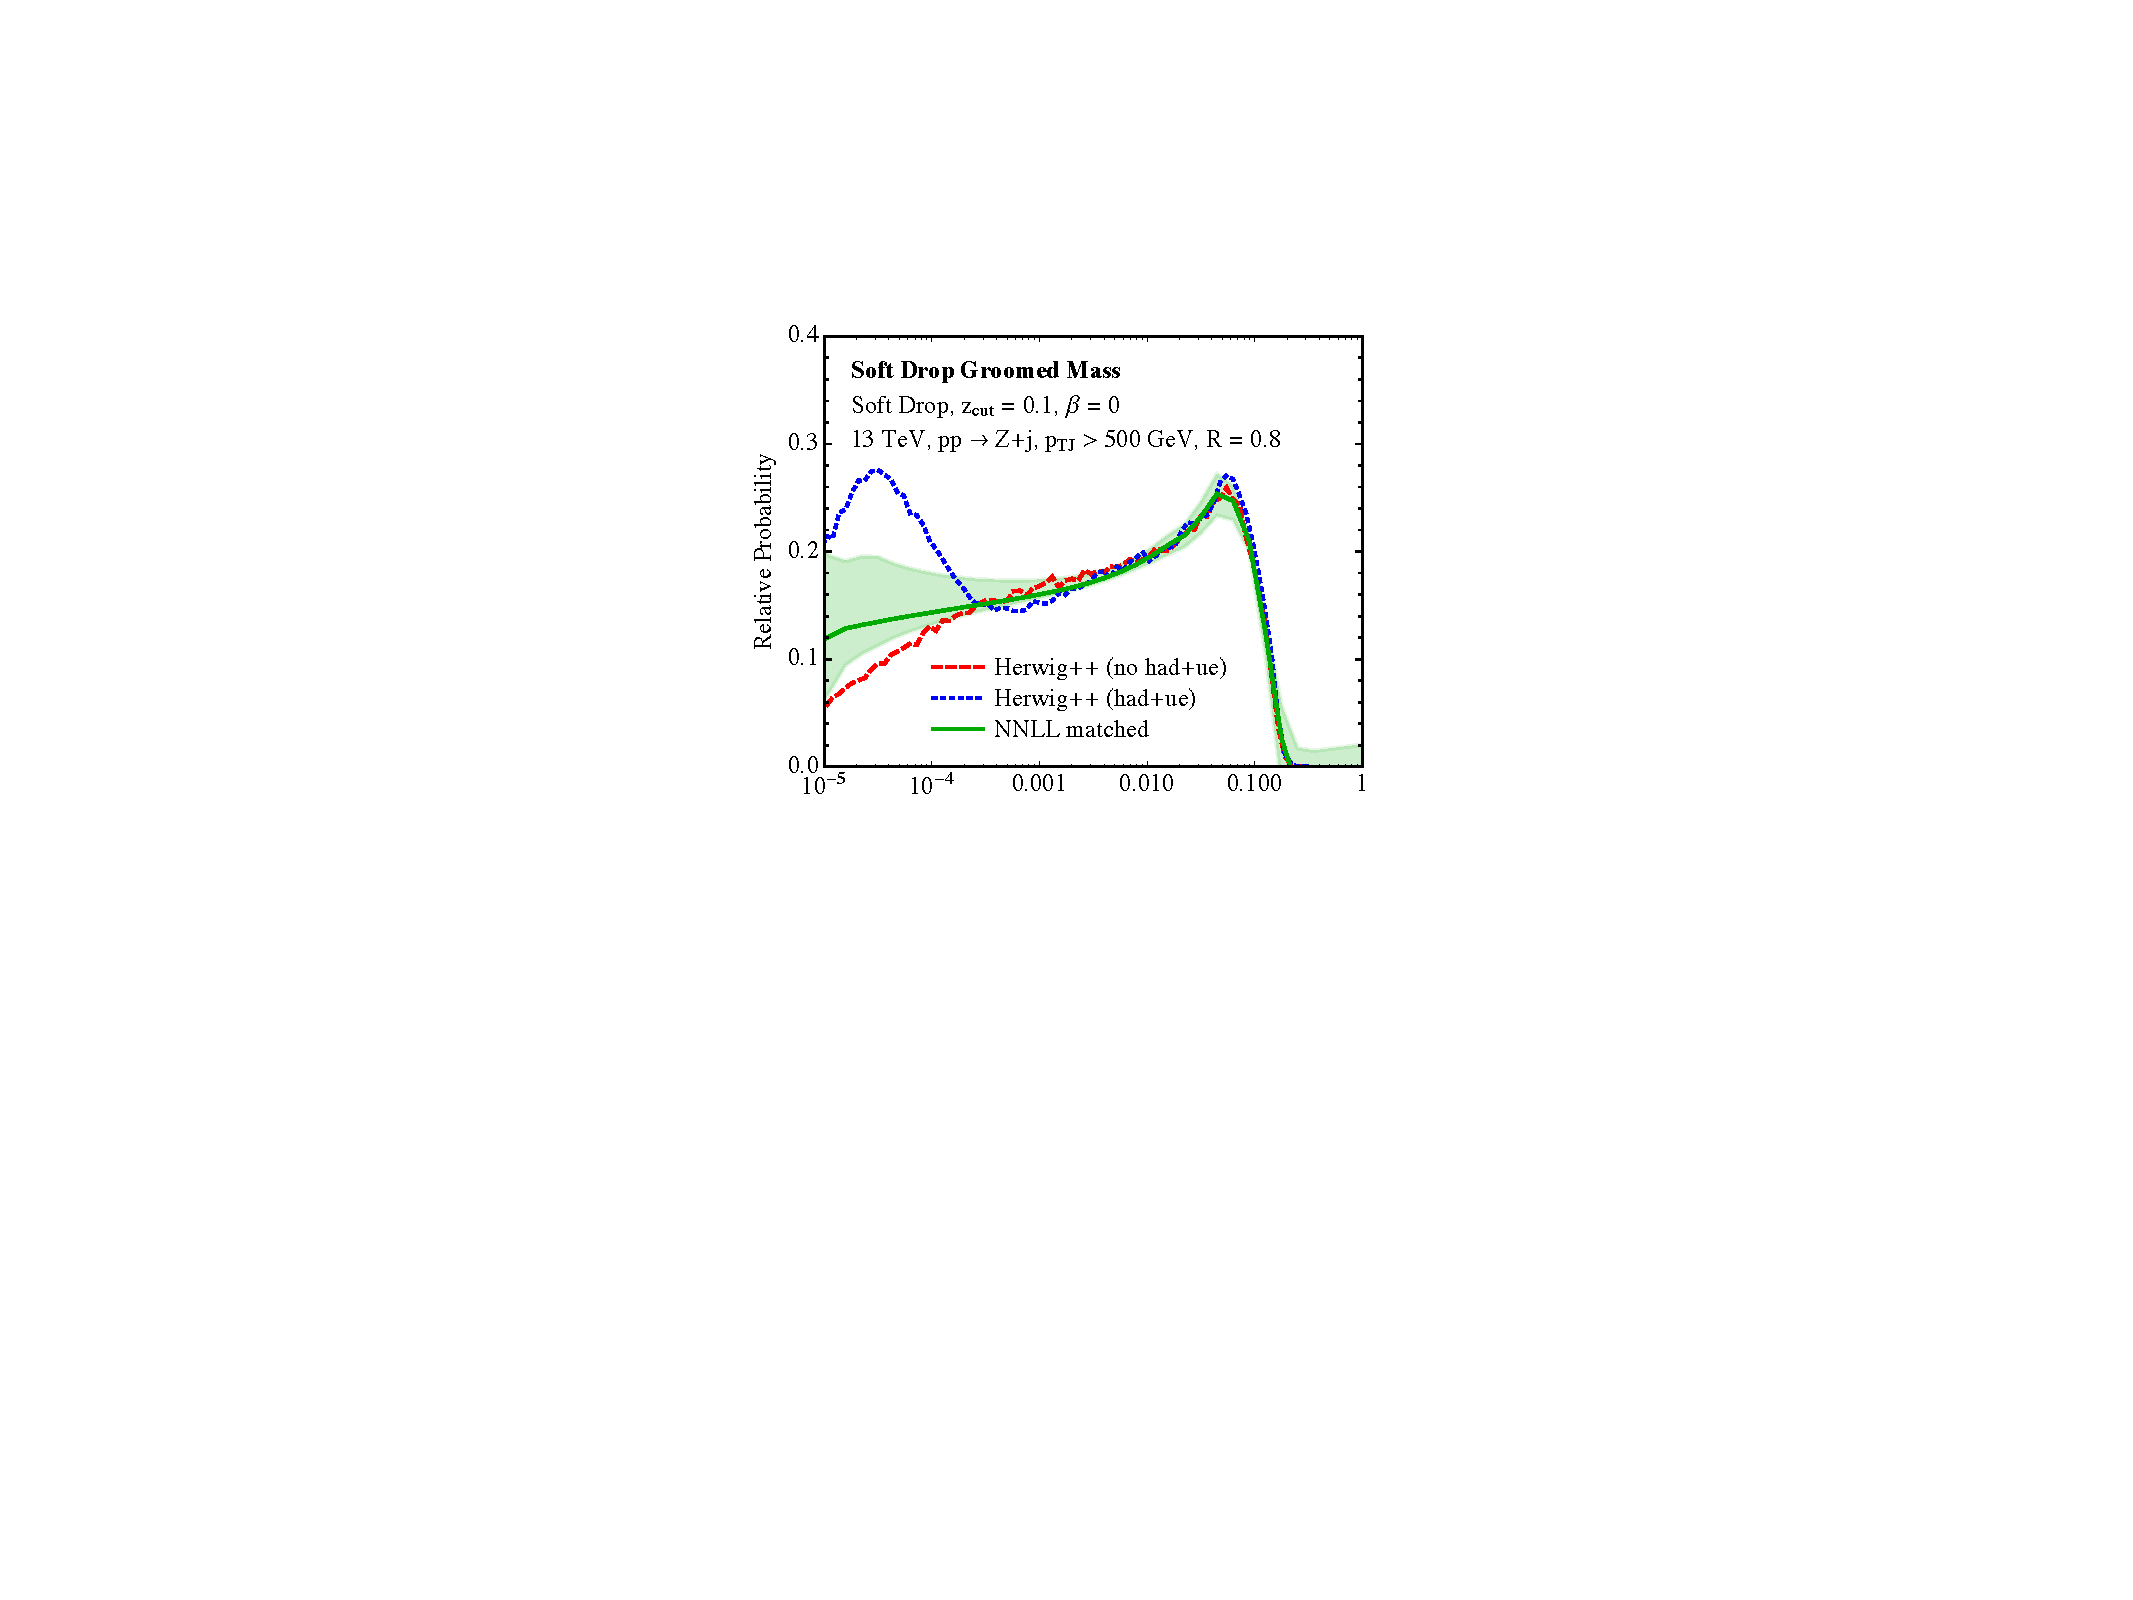
\includegraphics[width=0.4\columnwidth]{figures/mass_placeholder}
\end{center}
\caption{Sensitivity of the groomed mass distributions to the polarization. For aggressive grooming, the grooming removes a larger fraction of transversely polarized $W$s than longitudinally polarized $W$s, due to their more asymmetric momentum sharing. (placeholder)}
\end{figure}

\begin{figure}
\begin{center}
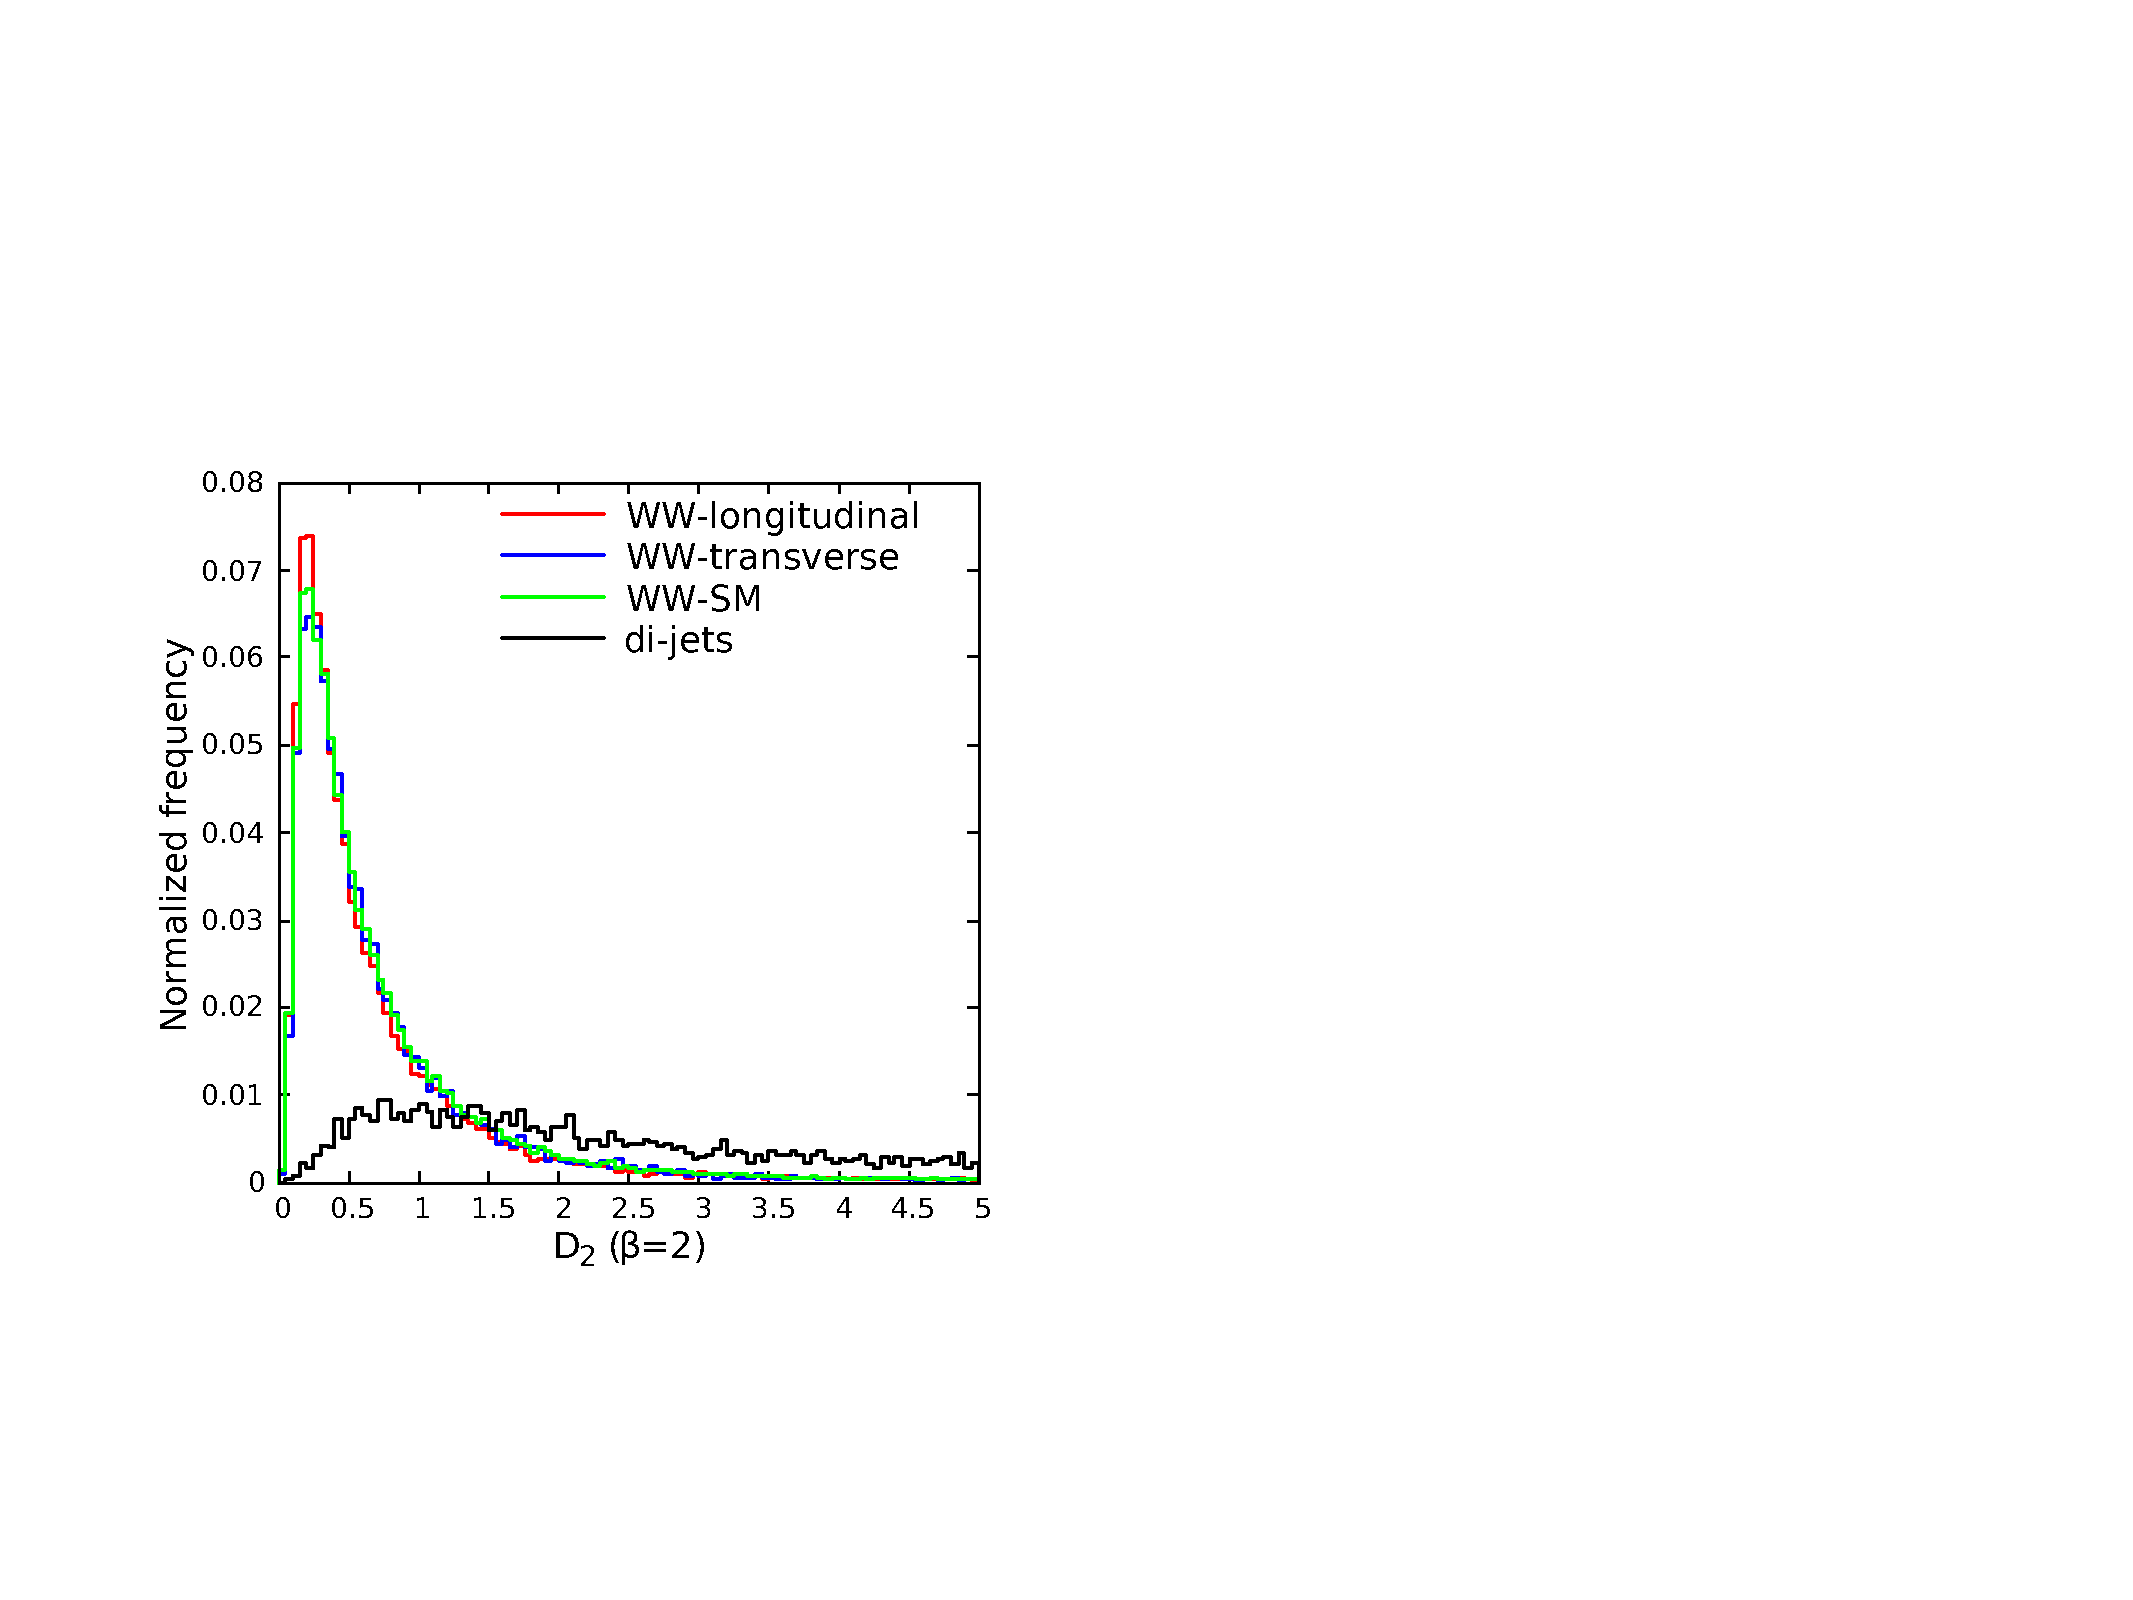
\includegraphics[width=0.3\columnwidth]{figures/D2_polarization}
\end{center}
\caption{Distributions of the $N_2$, $D_2$ and $\tau_{21}$ observables as measured on the samples with different polarization compositions. These observables are found to be largely insensitive to the polarization.}
\end{figure}

\begin{figure}
\begin{center}
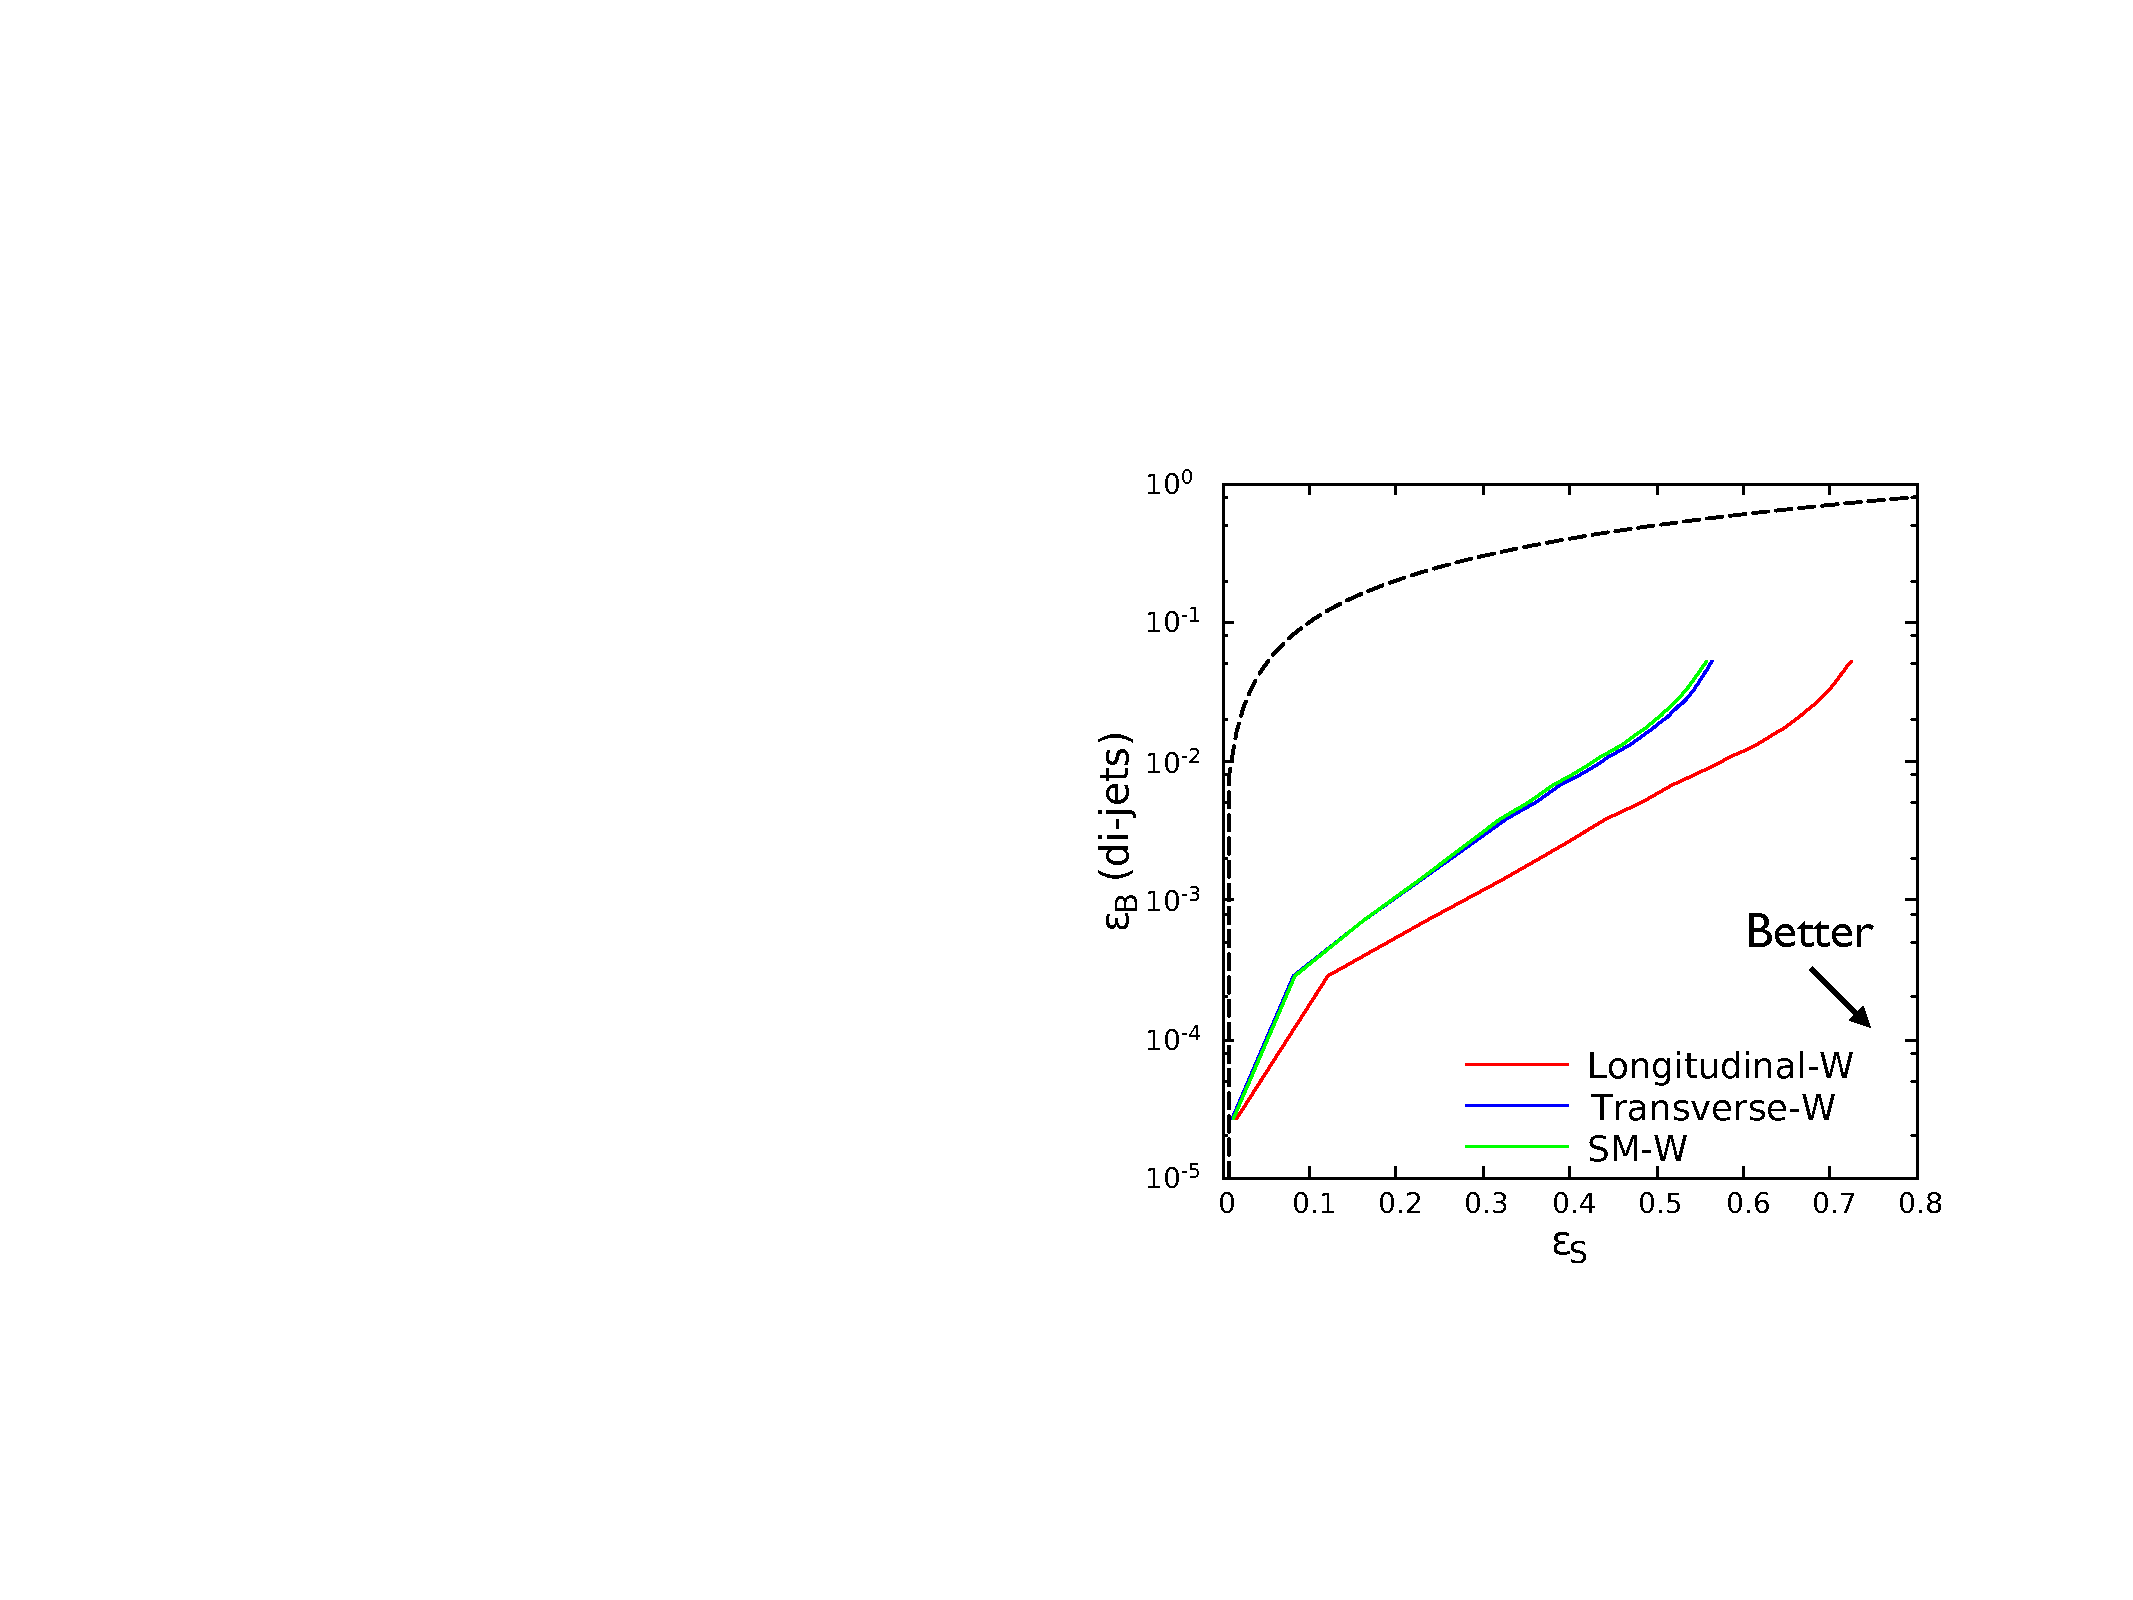
\includegraphics[width=0.3\columnwidth]{figures/ROC_polarization}
\end{center}
\caption{ROC curves comparing the different grooming strategies for different polarization samples. While the polarization has a limited effect on the jet shape observables, it modifies the groomed mass acceptance, and therefore the tagging efficiency, significantly.}
\end{figure}

%%%%%%%%%%%%%%%%%%%%%%%%%%%%%%%%%%%%%%%
\subsection{Tagging Polarization}\label{sec:polar_tag}
%%%%%%%%%%%%%%%%%%%%%%%%%%%%%%%%%%%%%%%



Having understood the robustness of the standard jet substructure observables to polarization, it is an interesting question to understand if jet substructure observables are able to tag distinct polarizations on hadronically decaying particles, and with what efficiency this can be done. Since the standard two prong tagging observables are not particularly sensitive to the polarization, a different observable must be used to tag polarizations. In this section we do not perform a comprehensive study, but restrict ourselves to studying a particular example of an observable which is sensitive to the $W$ polarization, and evaluate its performance for distinguishing transverse and longitudinal $W$ bosons. 

As discussed in \Sec{sec:polar_physics} the sole impact of the polarization of the decaying object is to determine the kinematics of the decaying subjets. Indeed, this can be made rigorous in the sense of a factorization theorem for boosted jets in the two-prong limit. We are therefore interested in an observable that is sensitive to the kinematics of the two subjets. While a variety of different observables could be considered, here we consider the $z_g$ observable \cite{Larkoski:2014wba,Larkoski:2014bia,Larkoski:2015lea}, which measures the momentum sharing of the subjets. The precise definition of $z_g$ was given in \Sec{sec:groom_tech}, which we recall for convenience
\begin{align}
z_g=\frac{\min\left[ p_{Ti}, p_{Tj}  \right]}{p_{Ti}+p_{Tj}}\,.
\end{align}

Since we are focused on robustness in this paper, it is also worth commenting on the robustness of the $z_g$ observable. For signal jets, since this observable measures global energy properties of the subjets, it is stable. Interestingly, it is also remarkably stable on the background, where it flows in the high $p_T$ limit to the QCD splitting function \cite{Larkoski:2014wba,Larkoski:2014bia,Larkoski:2015lea}.



\begin{figure}
\begin{center}
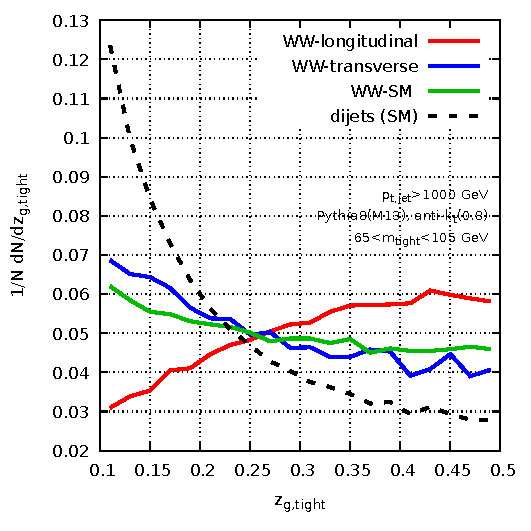
\includegraphics[width=0.45\columnwidth]{figures/polarisation-zg-distrib}
\end{center}
\caption{The $z_g$ distribution as measured on boosted $W$ samples with different polarization compositions. Transversely polarized $W$s behave similarly to the QCD background, while decent separation is observed between longitudinally polarized $W$s and transversely polarized $W$s.}
\label{z_g_dist}
\end{figure}

\begin{figure}
\begin{center}
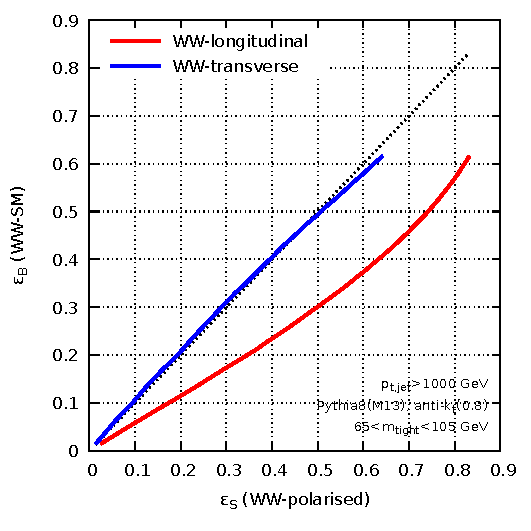
\includegraphics[width=0.45\columnwidth]{figures/polarisation-zg-roc}
\end{center}
\caption{A ROC curve showing the separation between transversely and longitudinally polarized $W$ bosons using the $z_g$ observable. Moderate separation is observed.}
\label{fig:z_g_ROC}
\end{figure}



%%%%%%%%%%%%%%%%%%%%%%%%%%%%%%%%%%%%%%%
\section{Theory Robustness}\label{sec:np}
%%%%%%%%%%%%%%%%%%%%%%%%%%%%%%%%%%%%%%%


In this section we study robustness to both hadronization, \Sec{sec:hadr}, and underlying event \Sec{sec:UE}, which we categorize as ``Theory" robustness, since both of these issues are present in a complete isolated hadronic collisions. Robustness to the detector, and pileup are treated in \Sec{sec:exp}. 



%%%%%%%%%%%%%%%%%%%%%%%%%%%%%%%%%%%%%%%
\subsection{Hadronization}\label{sec:hadr}
%%%%%%%%%%%%%%%%%%%%%%%%%%%%%%%%%%%%%%%





\begin{figure}
\begin{center}
\subfloat[]{\label{fig:unsoftdropped}
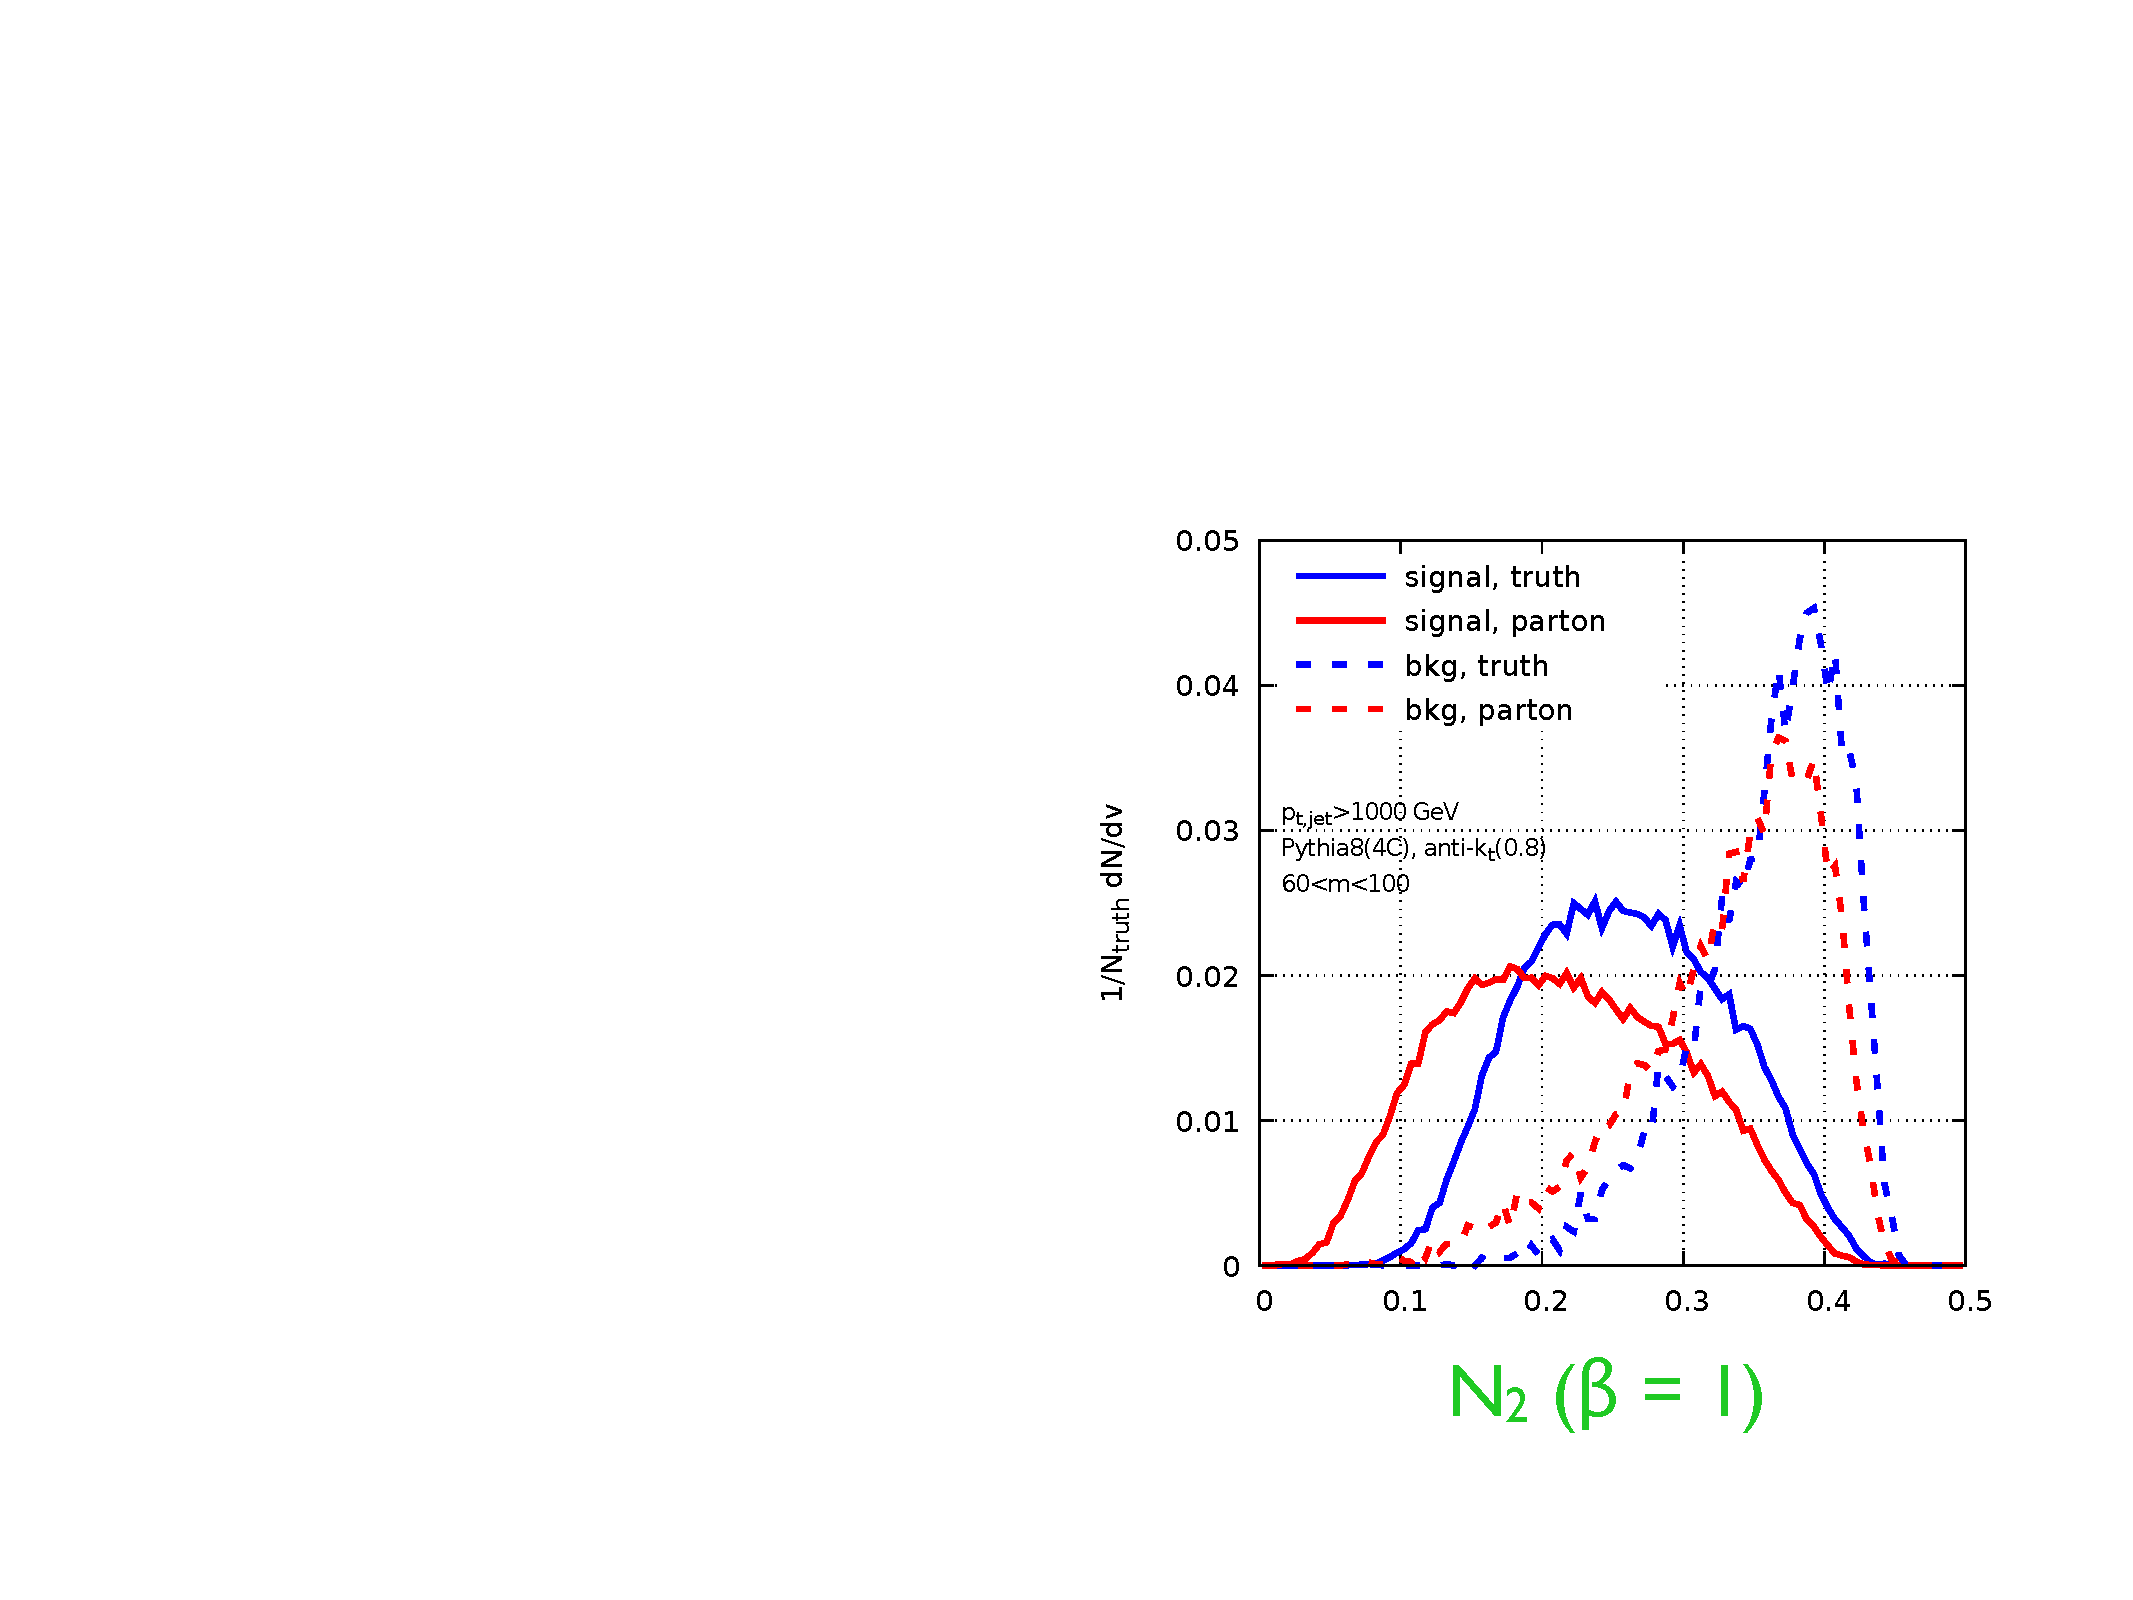
\includegraphics[width=7cm]{figures/N2_UE_dist}    
}\qquad
\subfloat[]{\label{fig:softdropped}
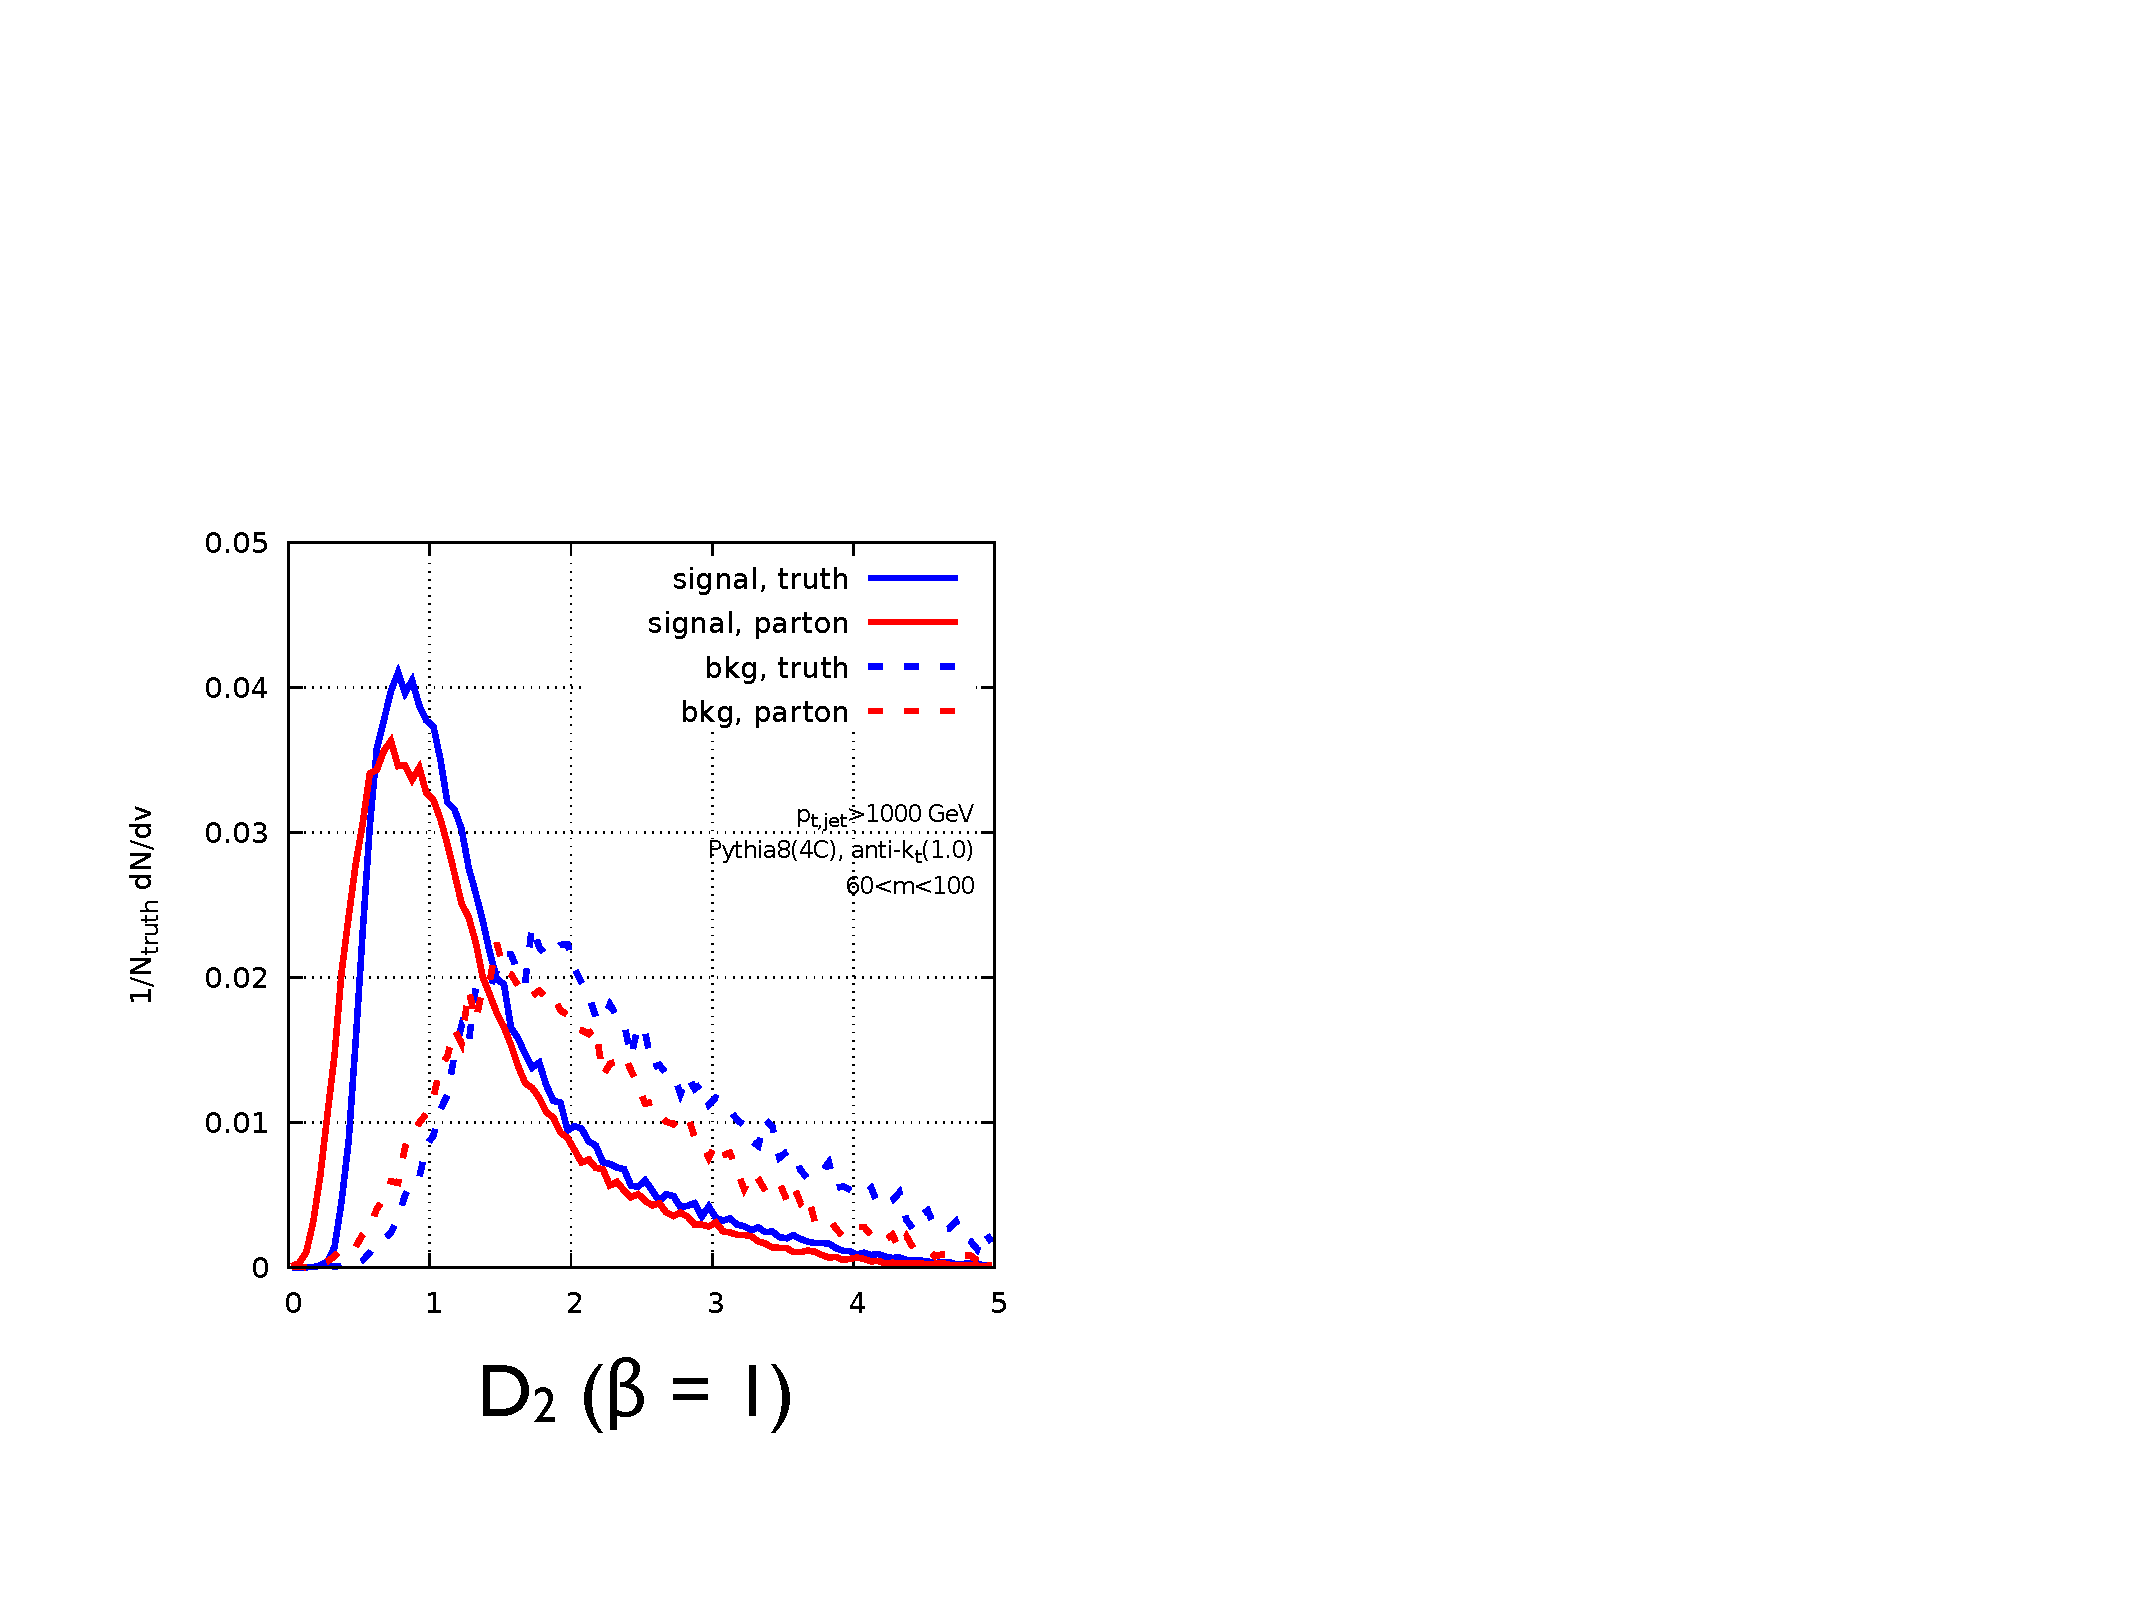
\includegraphics[width=7cm]{figures/D2_UE_dist}
}
\end{center}
\caption{ 
}
\label{fig:UE}
\end{figure}

In this section we study the robustness of the different tagging techniques to hadronization. As discussed in \Sec{sec:pres} this must be interpreted with some care, since the unhadronized events are not themselves physical. Nevertheless, the comparison of hadronized and unhadronized distributions is the best proxy for understand the impact of hadronization, short of performing an analytic calculation. To ensure that are conclusions are robust, we consider both the \pythia and \herwig Monte Carlos, which implement different hadronization models. The \pythia shower uses the string model \cite{Andersson:1983ia,Andersson:1998tv}, while \herwig uses the cluster model \cite{Webber:1983if,Marchesini:1987cf}. See for example \Refs{Buckley:2011ms,Skands:2011pf,Skands:2012ts} for a more detailed discussion. The effect of hadronization on two prong substructure observables has been studied in \cite{Larkoski:2015kga,Salam:2016yht}.


\ijm{have some plots, have some ROC curves. Not much else to say until then.}

%%%%%%%%%%%%%%%%%%%%%%%%%%%%%%%%%%%%%%%
\subsection{Underlying Event}\label{sec:UE}
%%%%%%%%%%%%%%%%%%%%%%%%%%%%%%%%%%%%%%%

Having understood the robustness of the observables to hadronization, we now consider underlying event...

\ijm{have some plots, have some ROC curves}

%%%%%%%%%%%%%%%%%%%%%%%%%%%%%%%%%%%%%%%
\section{Experimental Robustness}\label{sec:exp}
%%%%%%%%%%%%%%%%%%%%%%%%%%%%%%%%%%%%%%%


\ijm{I have nothing here.}   \ijm{can skip the detector robustness if need be for time}

%%%%%%%%%%%%%%%%%%%%%%%%%%%%%%%%%%%%%%%
\subsection{Detector Robustness}\label{sec:detector_robust}
%%%%%%%%%%%%%%%%%%%%%%%%%%%%%%%%%%%%%%%

\ijm{discuss detector effects}

%%%%%%%%%%%%%%%%%%%%%%%%%%%%%%%%%%%%%%%
\subsection{Pile-Up Robustness}\label{sec:pu_robust}
%%%%%%%%%%%%%%%%%%%%%%%%%%%%%%%%%%%%%%%

\ijm{show plots as a function of pile up}

%%%%%%%%%%%%%%%%%%%%%%%%%%%%%%%%%%%%%%%
\subsection{Tagging at Extreme $p_T$}\label{sec:pt_robust}
%%%%%%%%%%%%%%%%%%%%%%%%%%%%%%%%%%%%%%%

\ijm{show plots as a function of $p_T$, degradation}

\begin{figure}
\begin{center}
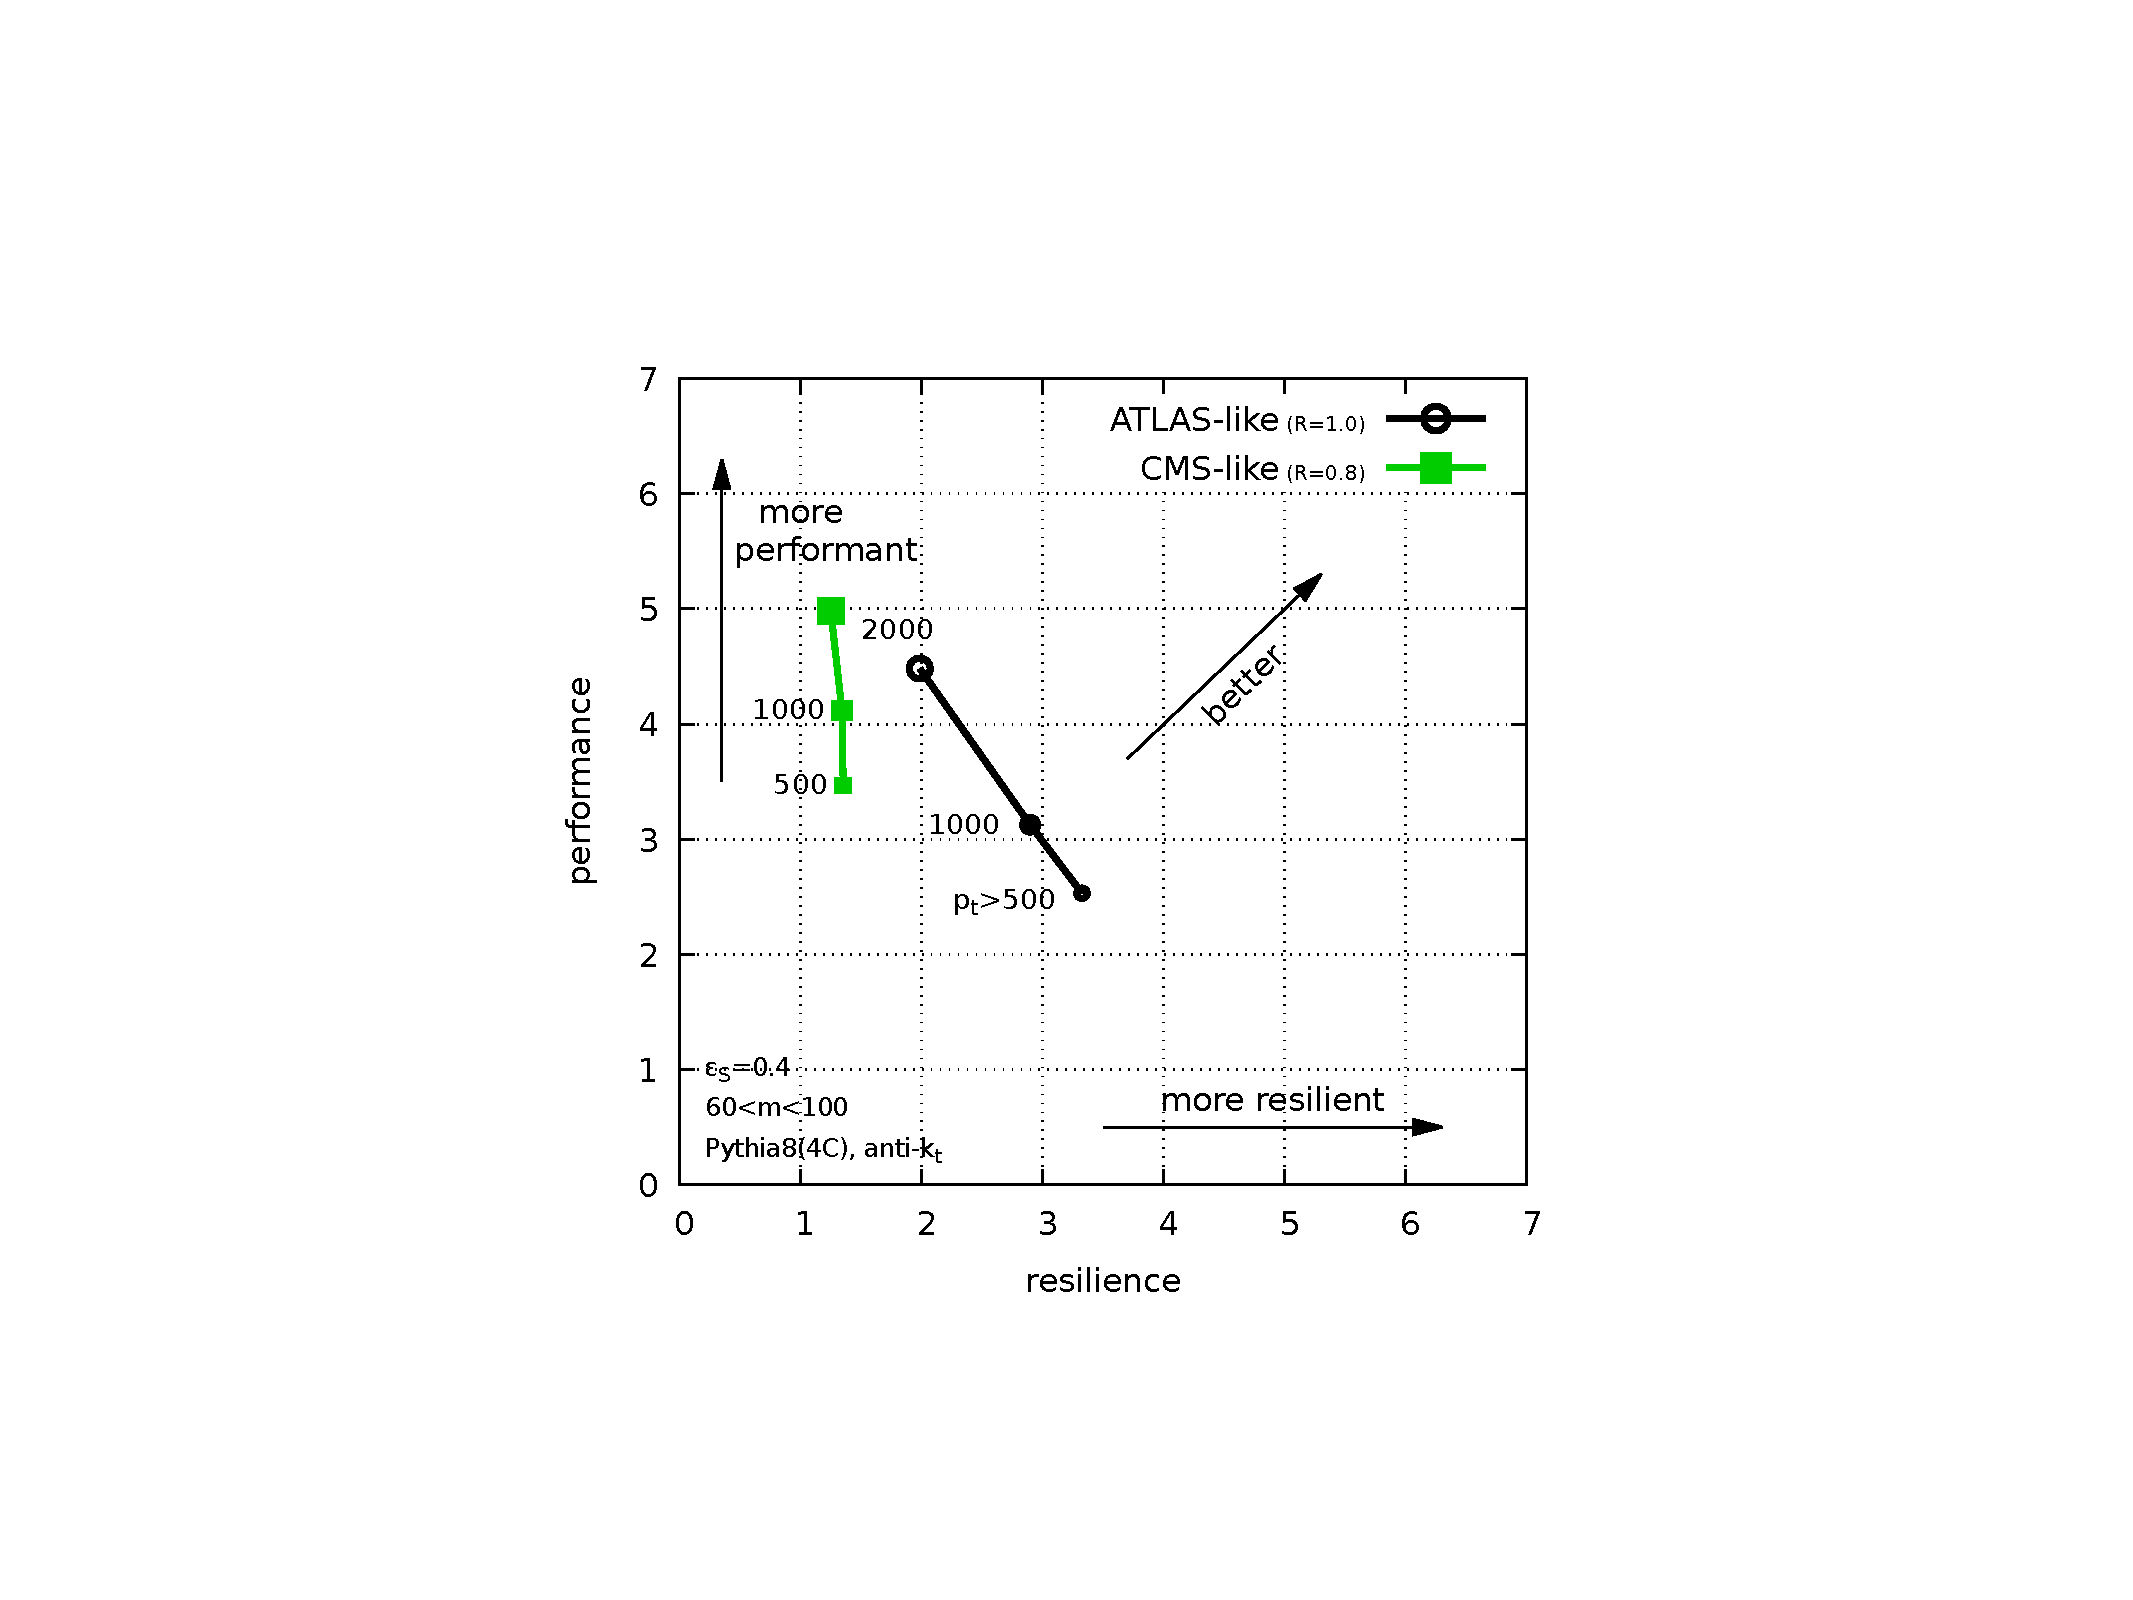
\includegraphics[width=0.4\columnwidth]{figures/sweep_pt}
\end{center}
\caption{sweeping pt}
\label{fig:nolabel}
\end{figure}

\begin{figure}
\begin{center}
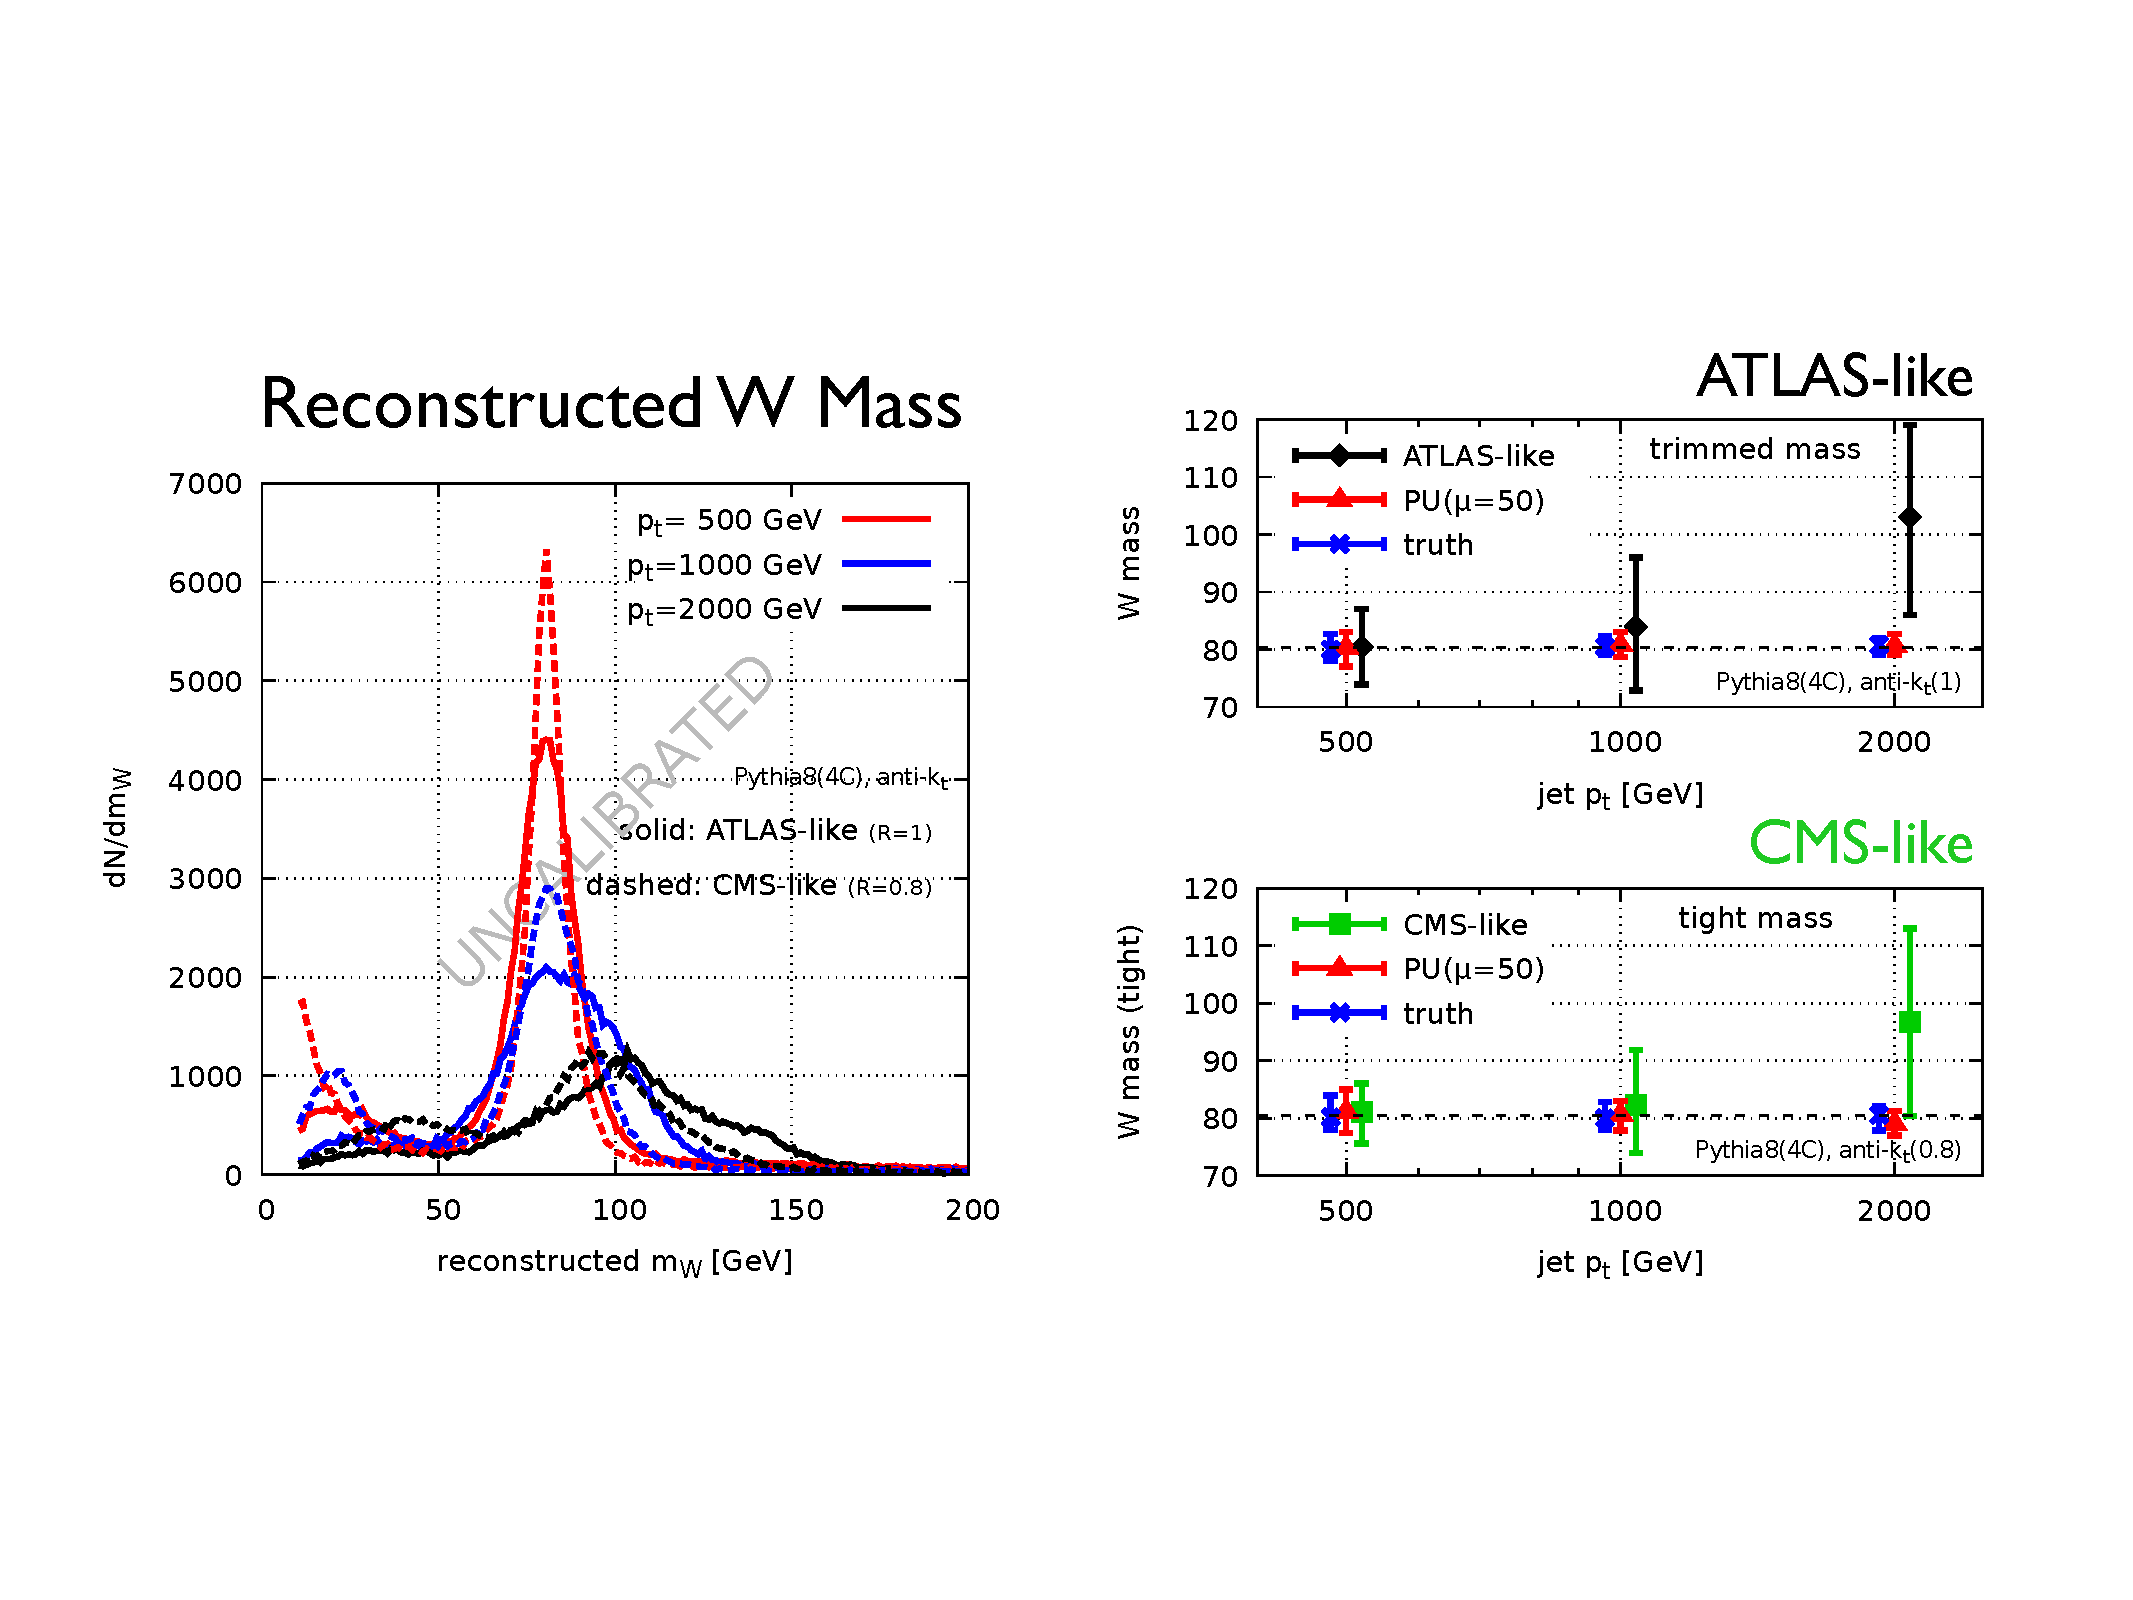
\includegraphics[width=0.75\columnwidth]{figures/pt_degrade}
\end{center}
\caption{Performance at high PT}
\label{fig:nolabel}
\end{figure}



\begin{figure}
\begin{center}
\subfloat[]{\label{fig:unsoftdropped}
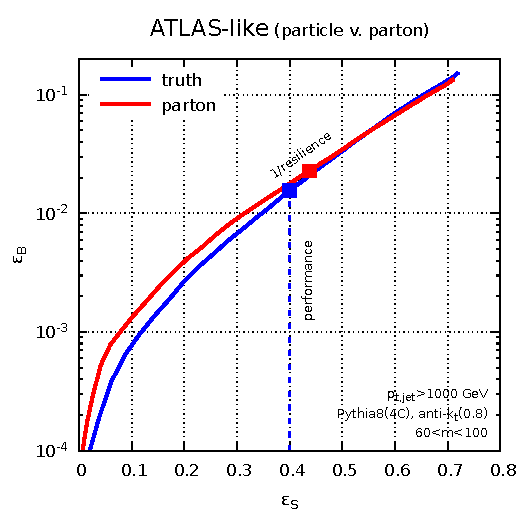
\includegraphics[width=7cm]{figures/default-rocs-R0pt8}    
}\qquad
\subfloat[]{\label{fig:softdropped}
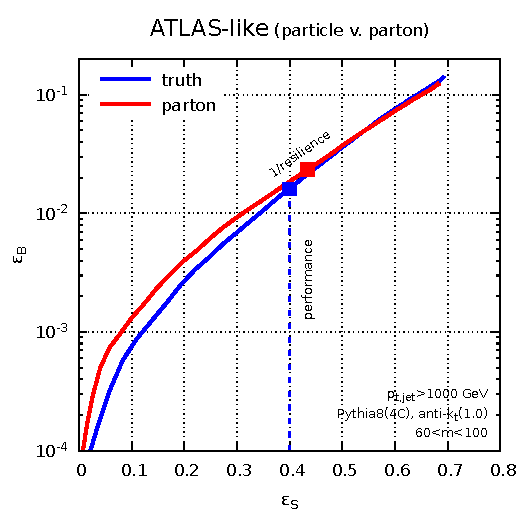
\includegraphics[width=7cm]{figures/default-rocs-R1pt0}
}
\end{center}
\caption{ATLAS vs. CMS
}
\label{fig:phasespace}
\end{figure}


\begin{figure}
\begin{center}
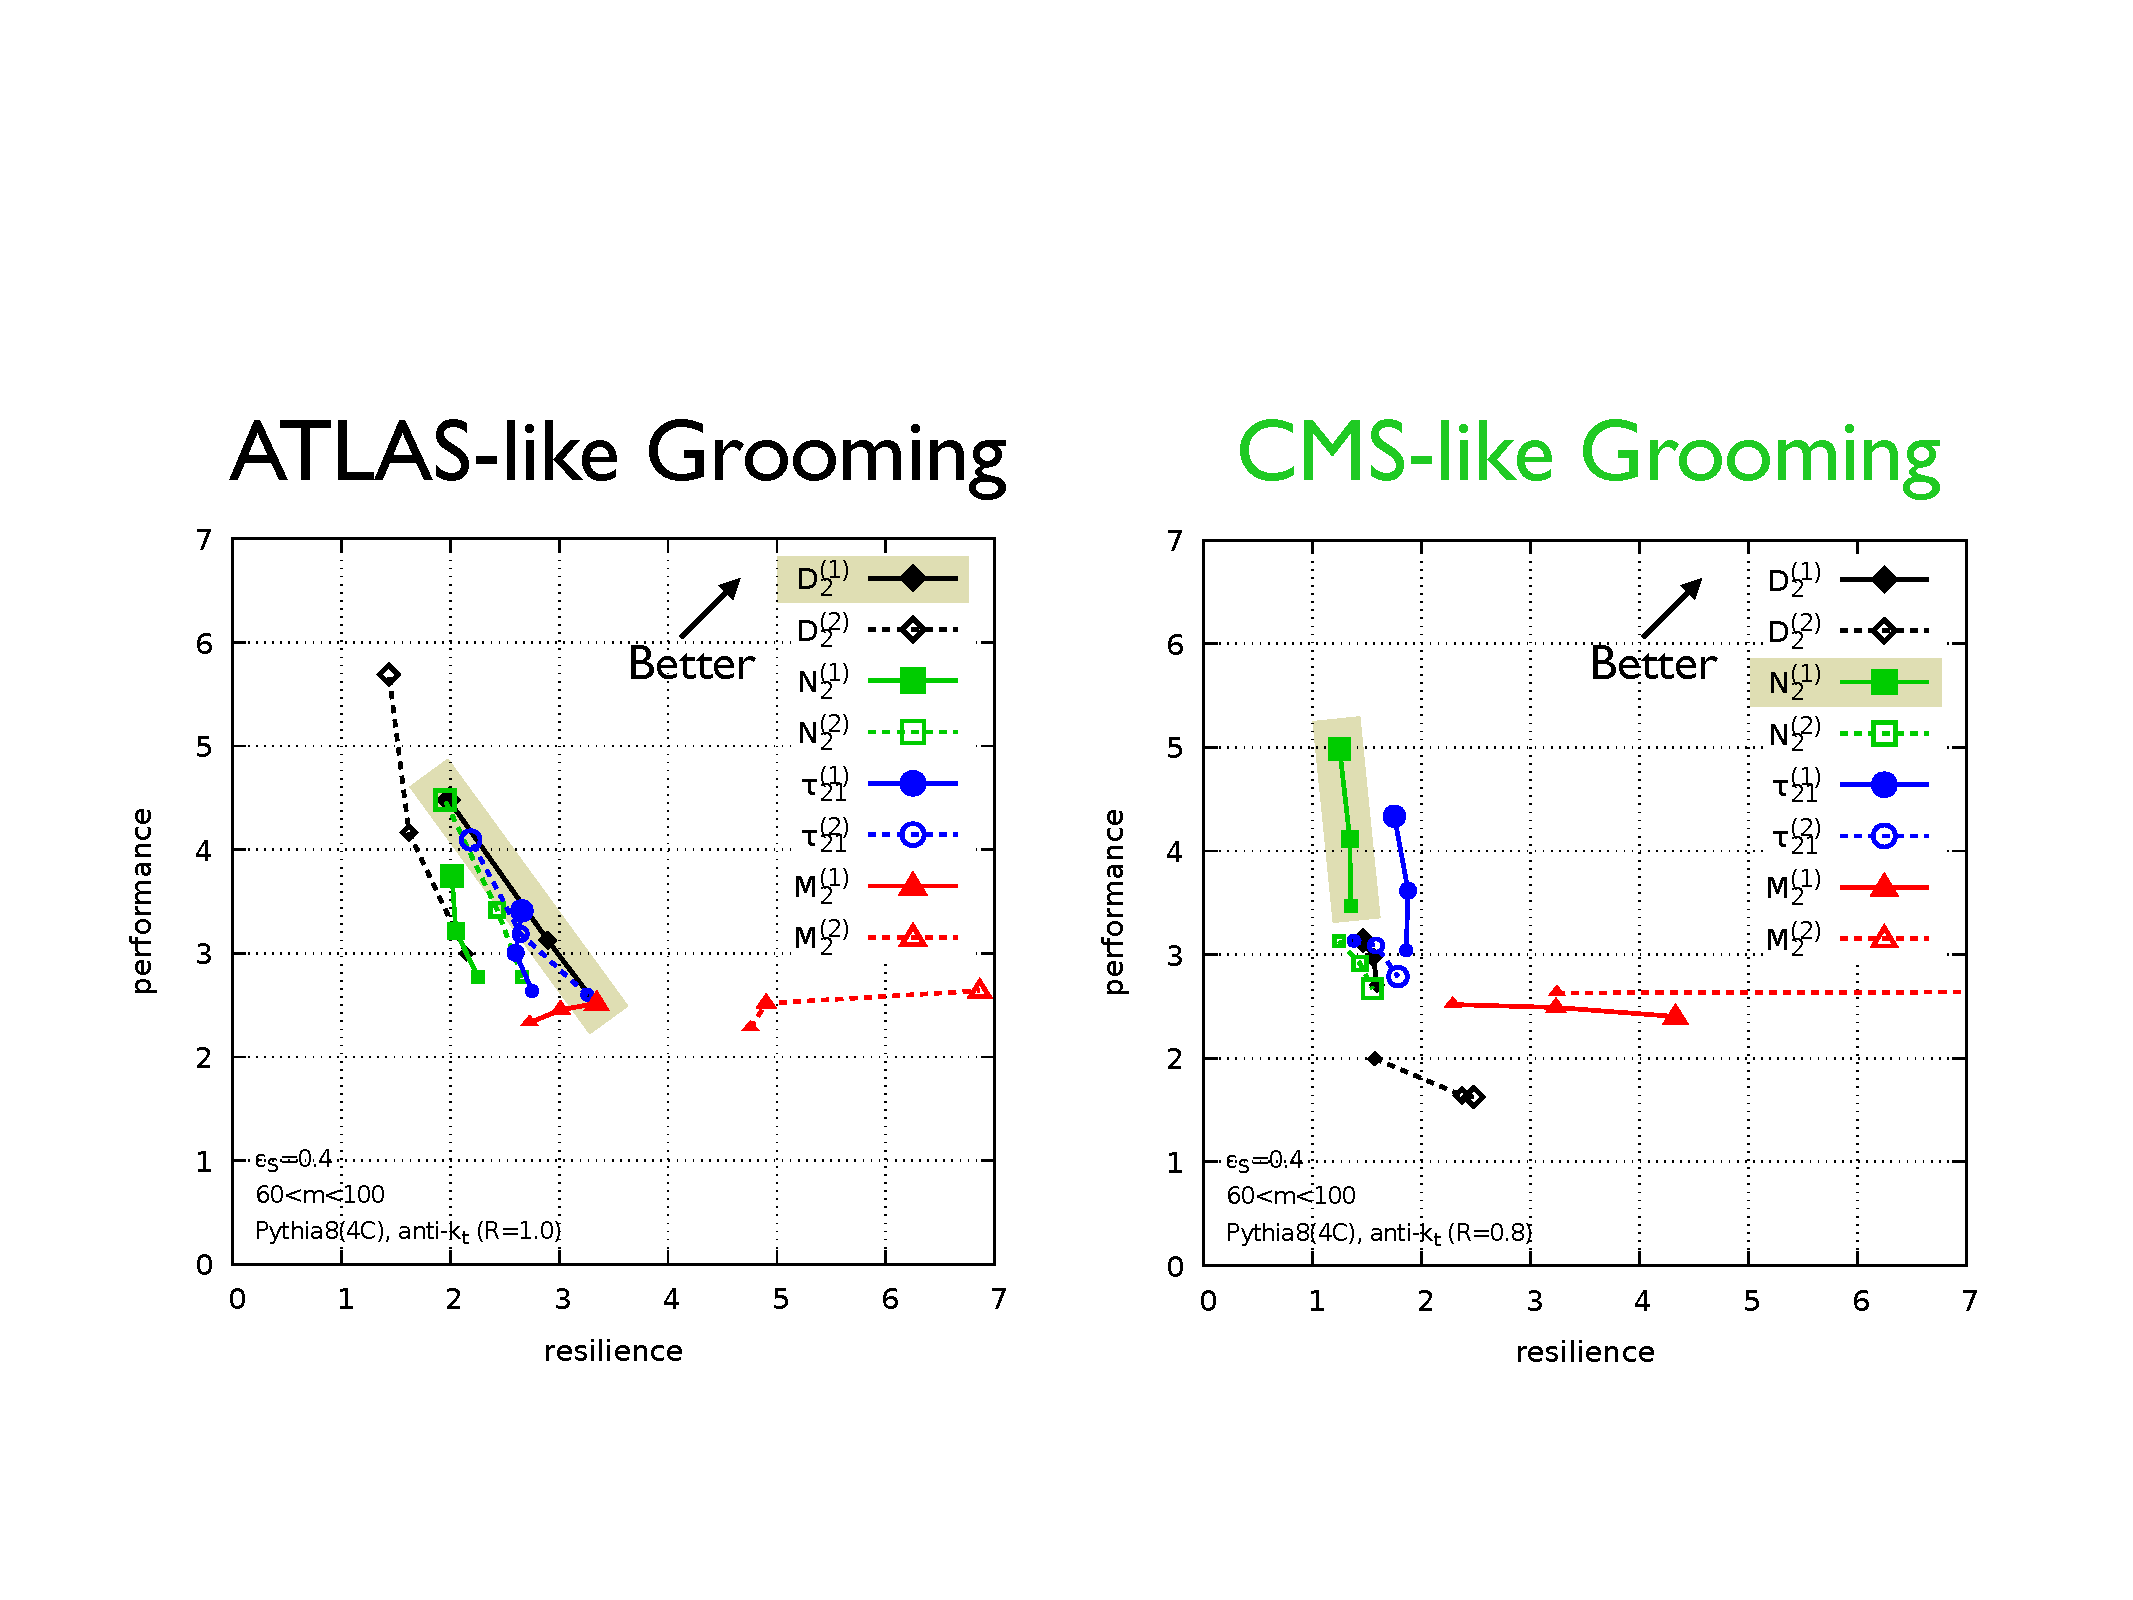
\includegraphics[width=0.75\columnwidth]{figures/sweep_obs}
\end{center}
\caption{sweeping observable}
\label{fig:nolabel}
\end{figure}

\begin{figure}
\begin{center}
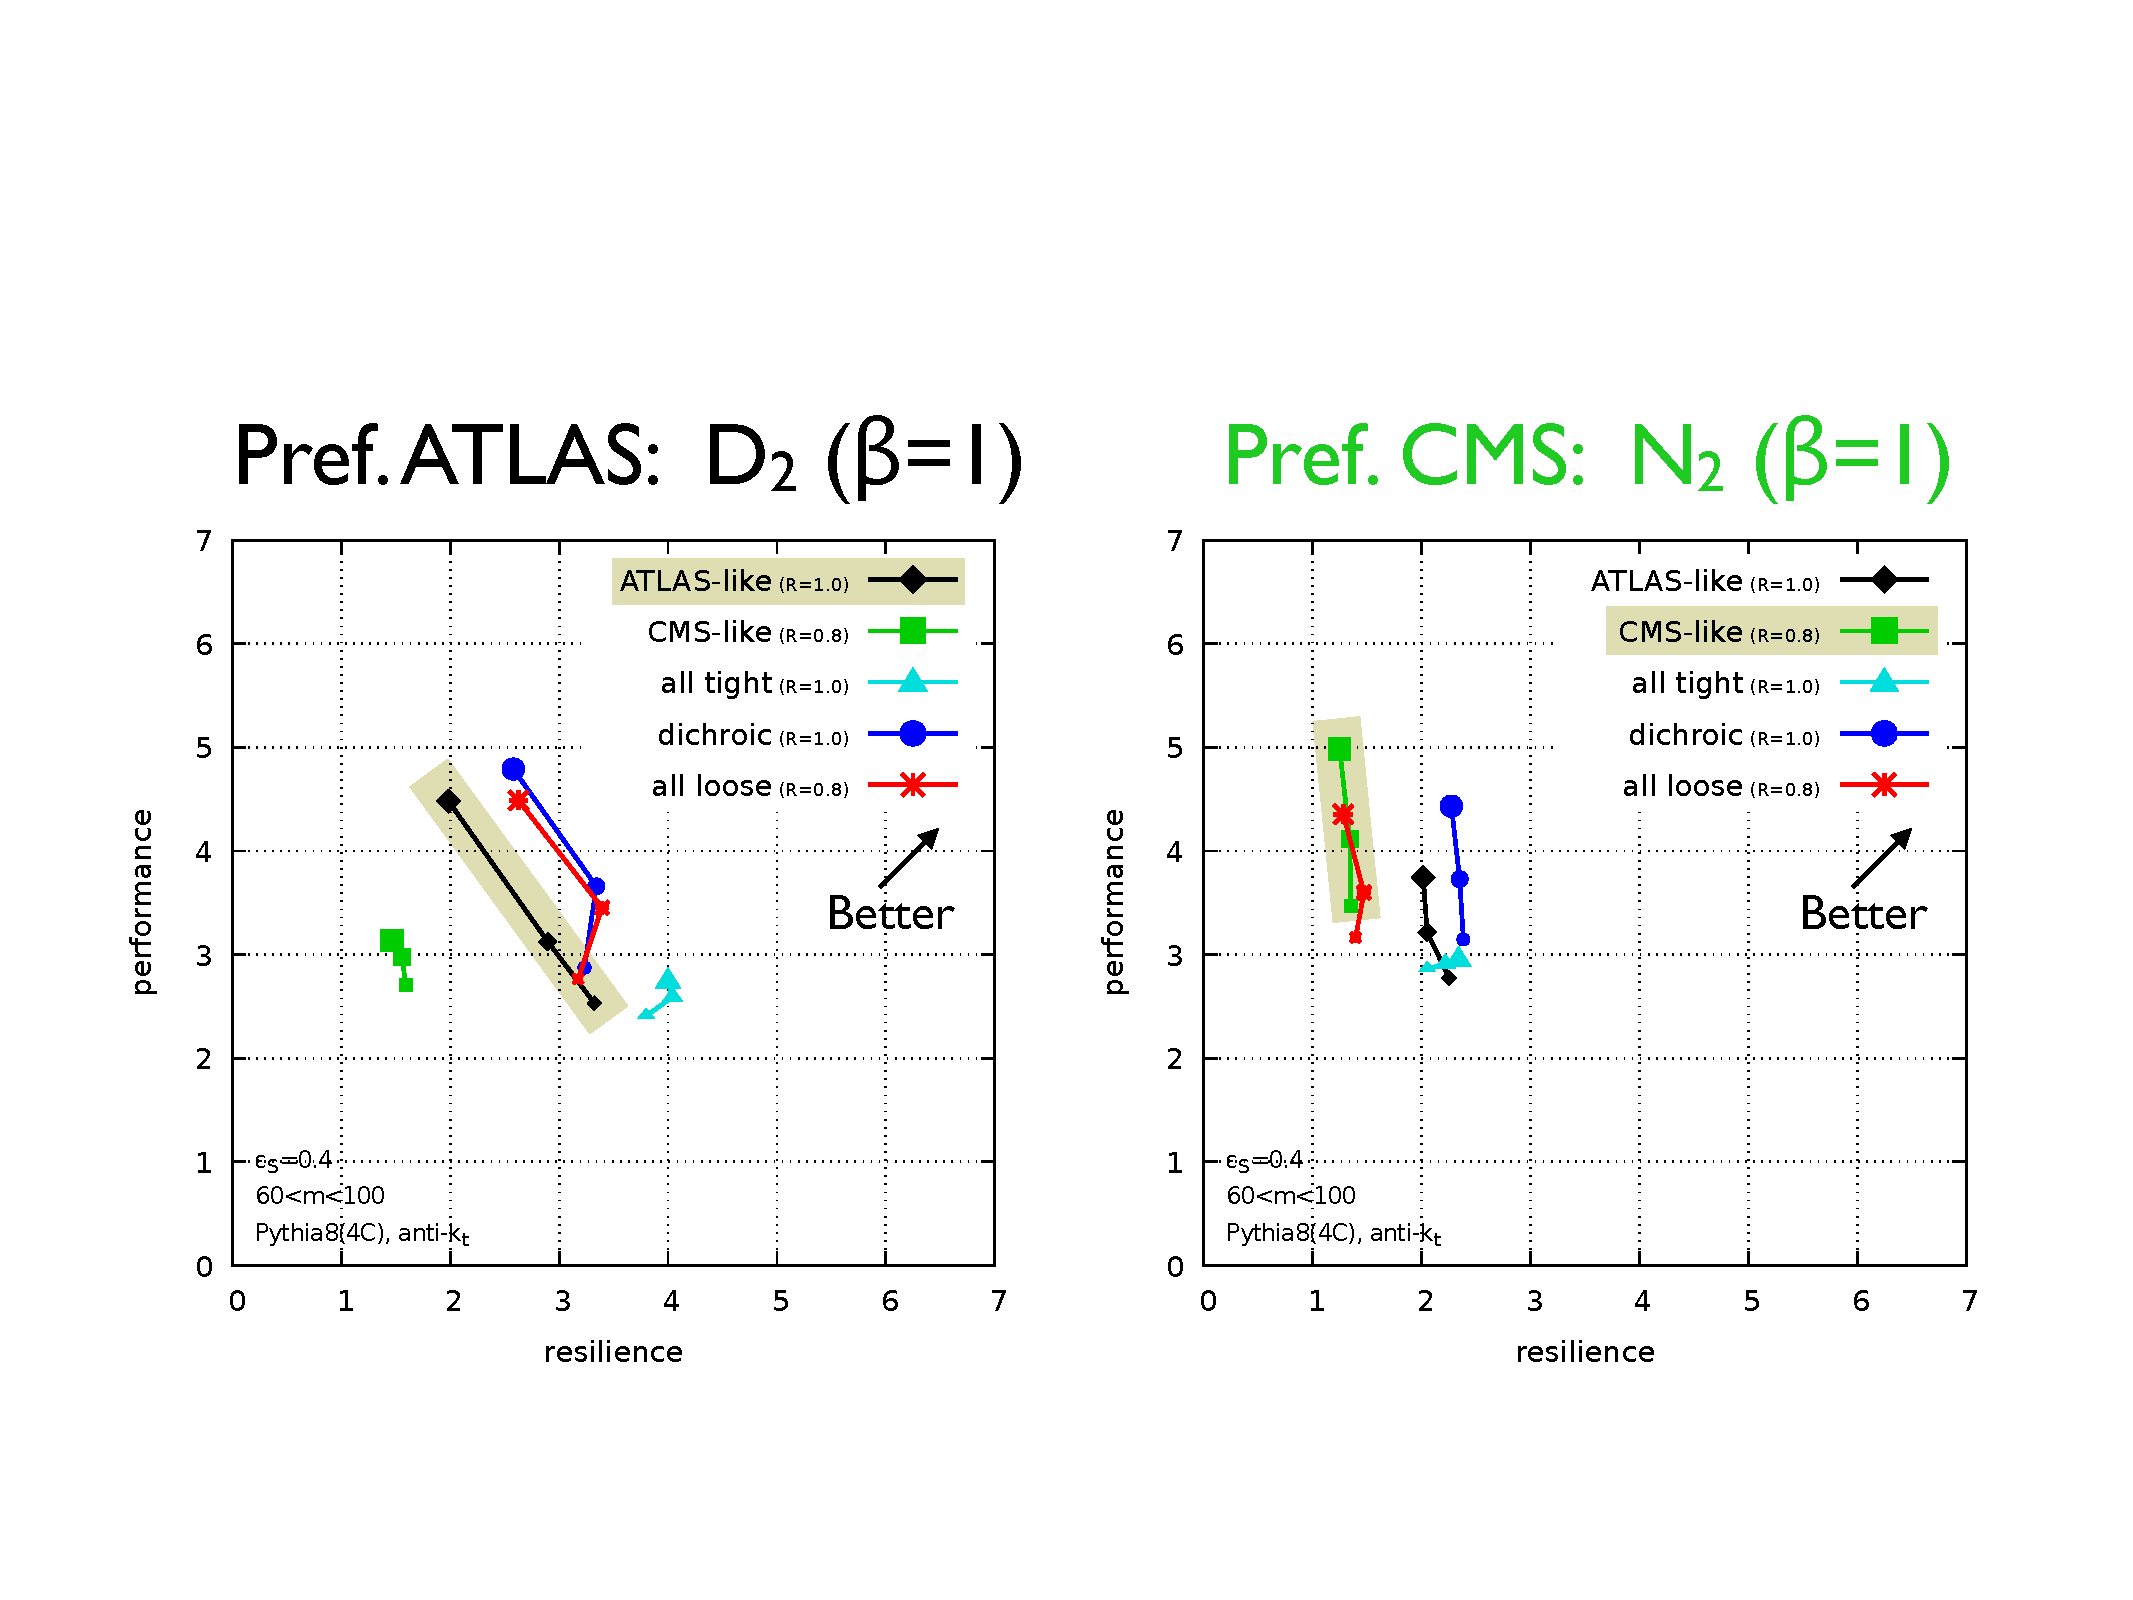
\includegraphics[width=0.75\columnwidth]{figures/sweep_groom}
\end{center}
\caption{sweeping groomer}
\label{fig:nolabel}
\end{figure}

%\section{Jet Radius Robustness:  High pT (isolation versus shape cut, jet radius)}

%\ijm{I think no longer have this in this separate section}




%%%%%%%%%%%%%%%%%%%%%%%%%%%%%%%%%%%%%
\section{Understanding Differences Between ATLAS and CMS}\label{sec:exp_compare}
%%%%%%%%%%%%%%%%%%%%%%%%%%%%%%%%%%%%%

The strategies used by ATLAS and CMS, namely trimmed  D2 \cite{Larkoski:2015kga}\cite{Larkoski:2014gra} and soft dropped N2 \cite{Moult:2016cvt} with DDT \cite{Dolen:2016kst} are specific examples of the broader approaches to two-prong tagging discussed above, and therefore our study allows us to gain insight into the different tagging strategies used by the collaborations.\footnote{And perhaps even into the sociology of the different experiments! However, such conclusions should be taken with a grain of salt.}

\ijm{I think for our purposes we can ignore the DDT. }

\ijm{this needs to be filled in once we have a more complete picture}


%%%%%%%%%%%%%%%%%%%%%%%%%%%%%%%%%%%%%%%
\section{Summary and Recommendations}\label{sec:conc}
%%%%%%%%%%%%%%%%%%%%%%%%%%%%%%%%%%%%%%%

In this paper, we have performed a comprehensive study of performance and robustness for two-prong tagging, and provided a unifying approach to understanding different approaches for two-prong tagging. 

similar approaches could also be applied to study $3$-prong tagging...


In all cases, we have identified taggers that outperform, in both robustness and tagging performance, those currently used by the ATLAS and CMS collaborations. We therefore believe that further studies using more detailed simulations of the ATLAS and CMS detectors, and ultimately on real data, would be of significant interest. More generally, we believe that the emphasis on a simultaneous evaluation of the performance and robustness, as well as the particular metrics introduced in this paper, will play a significant role in future studies of jet substructure techniques at the LHC.

\ijm{this needs to be filled in once we have a more complete picture}




\begin{figure}
\begin{center}
\subfloat[]{\label{fig:unsoftdropped}
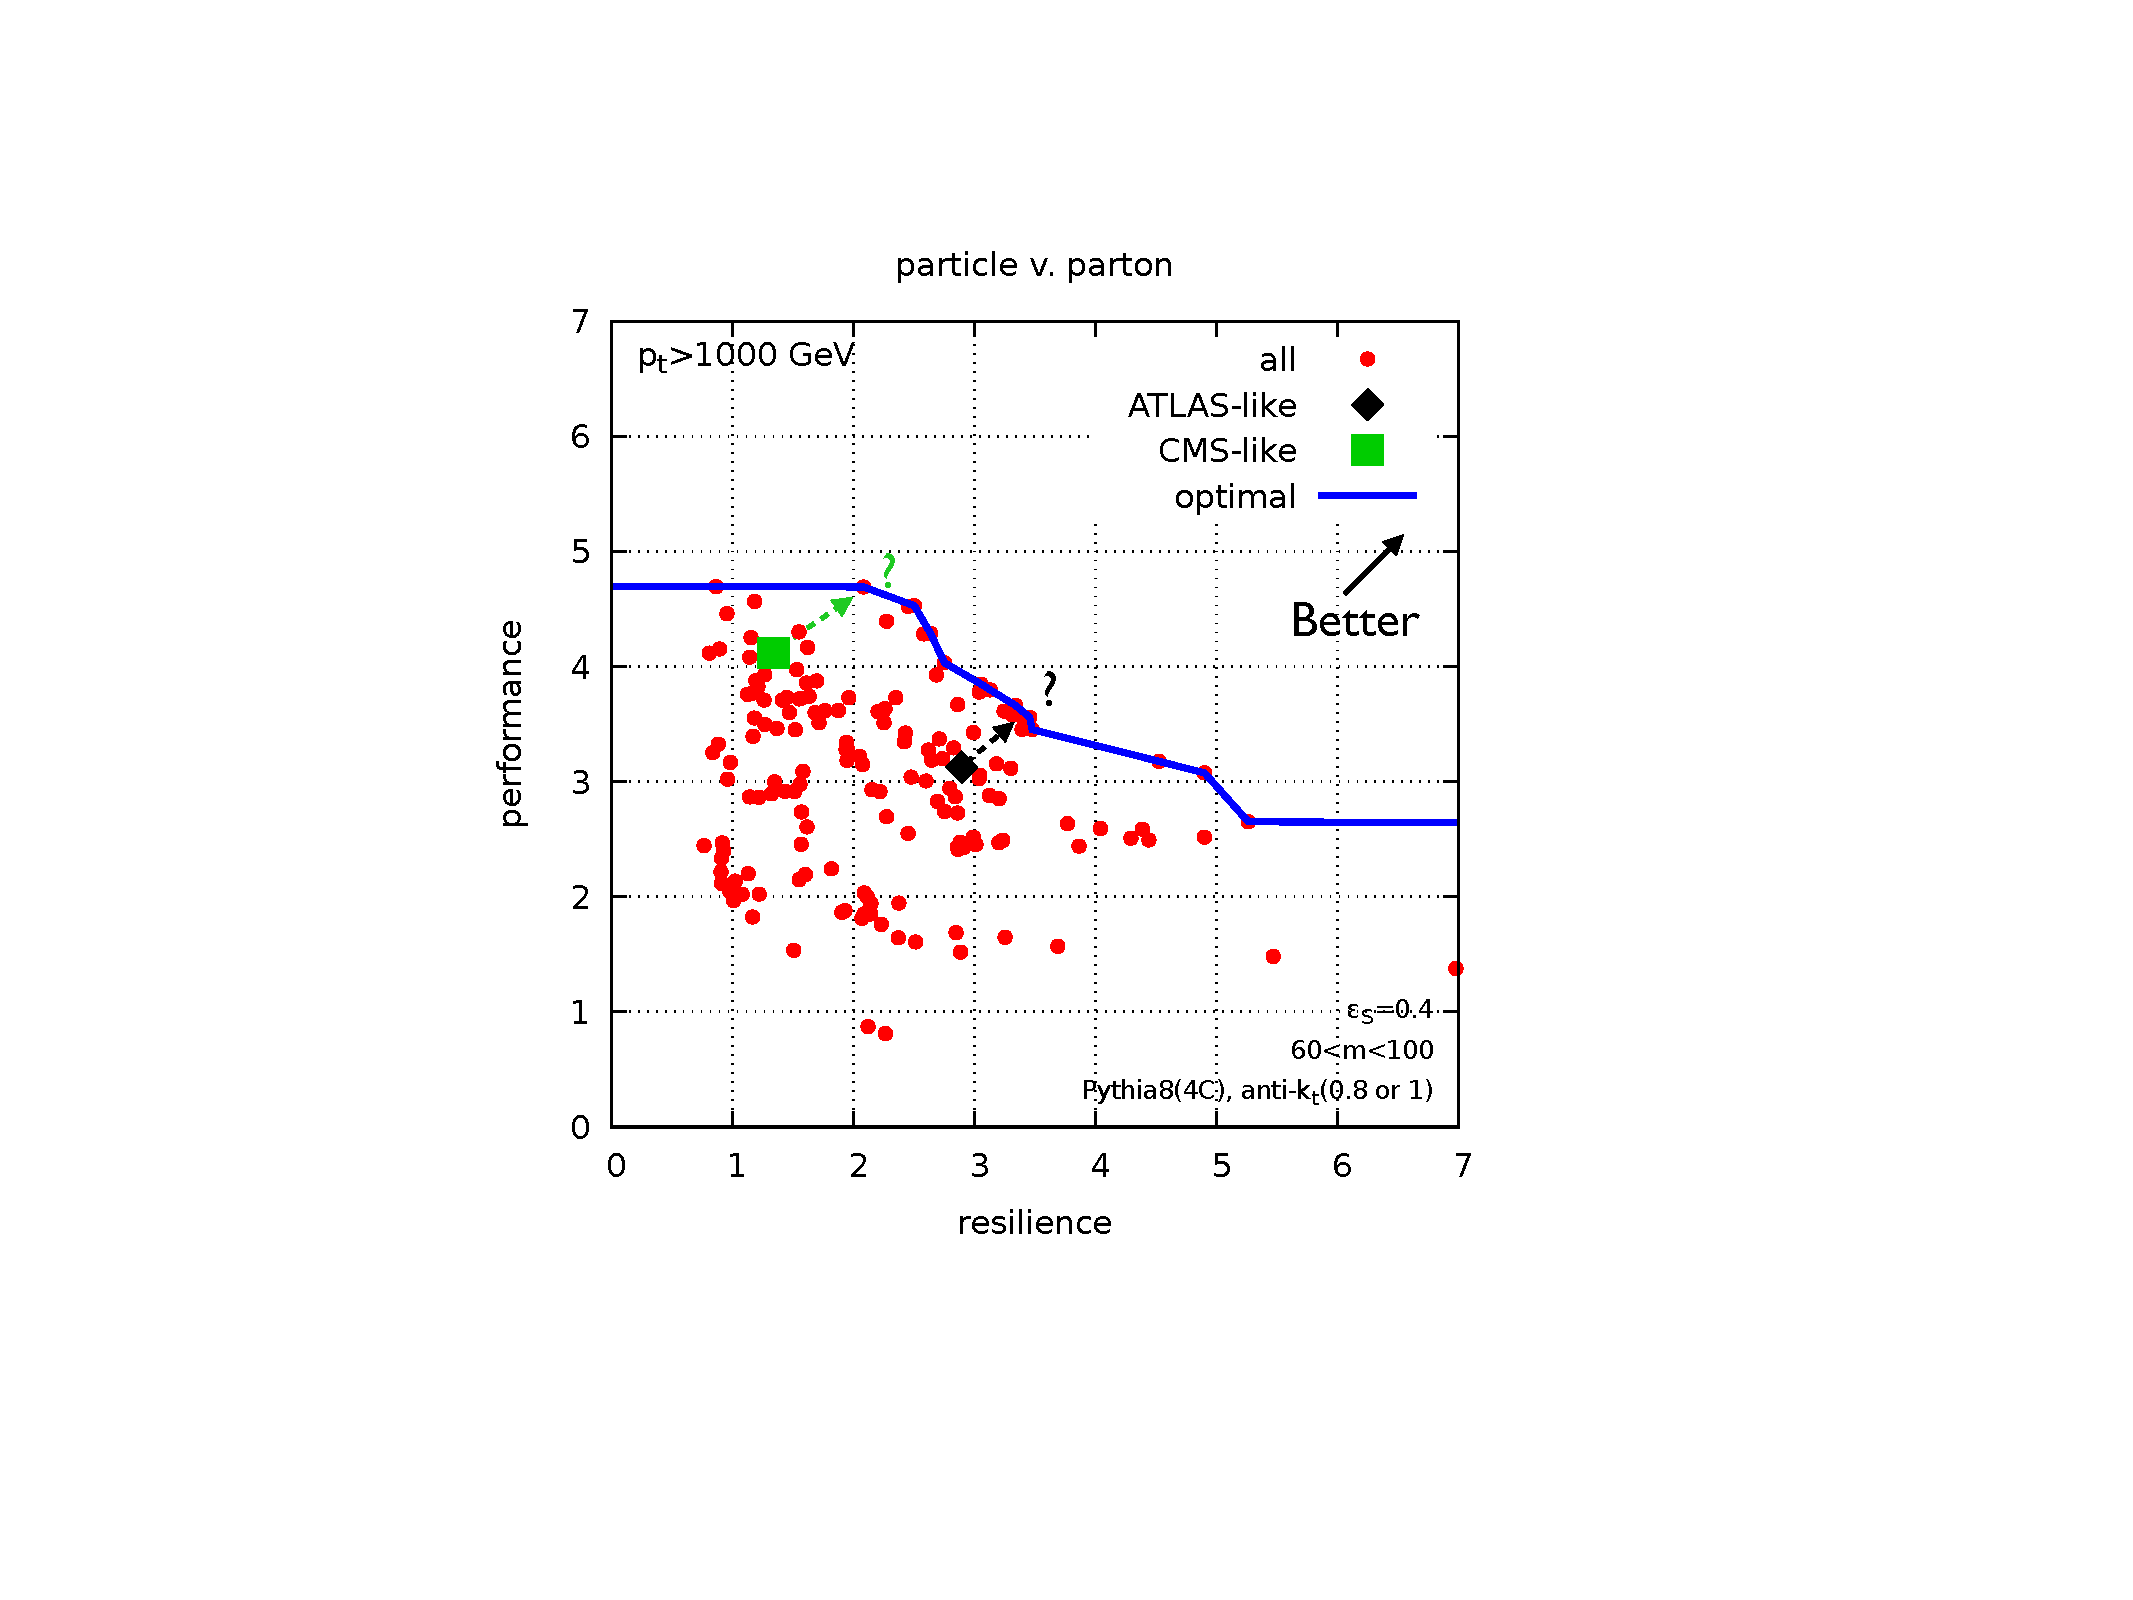
\includegraphics[width=7cm]{figures/resilience_summary}    
}\qquad
\subfloat[]{\label{fig:softdropped}
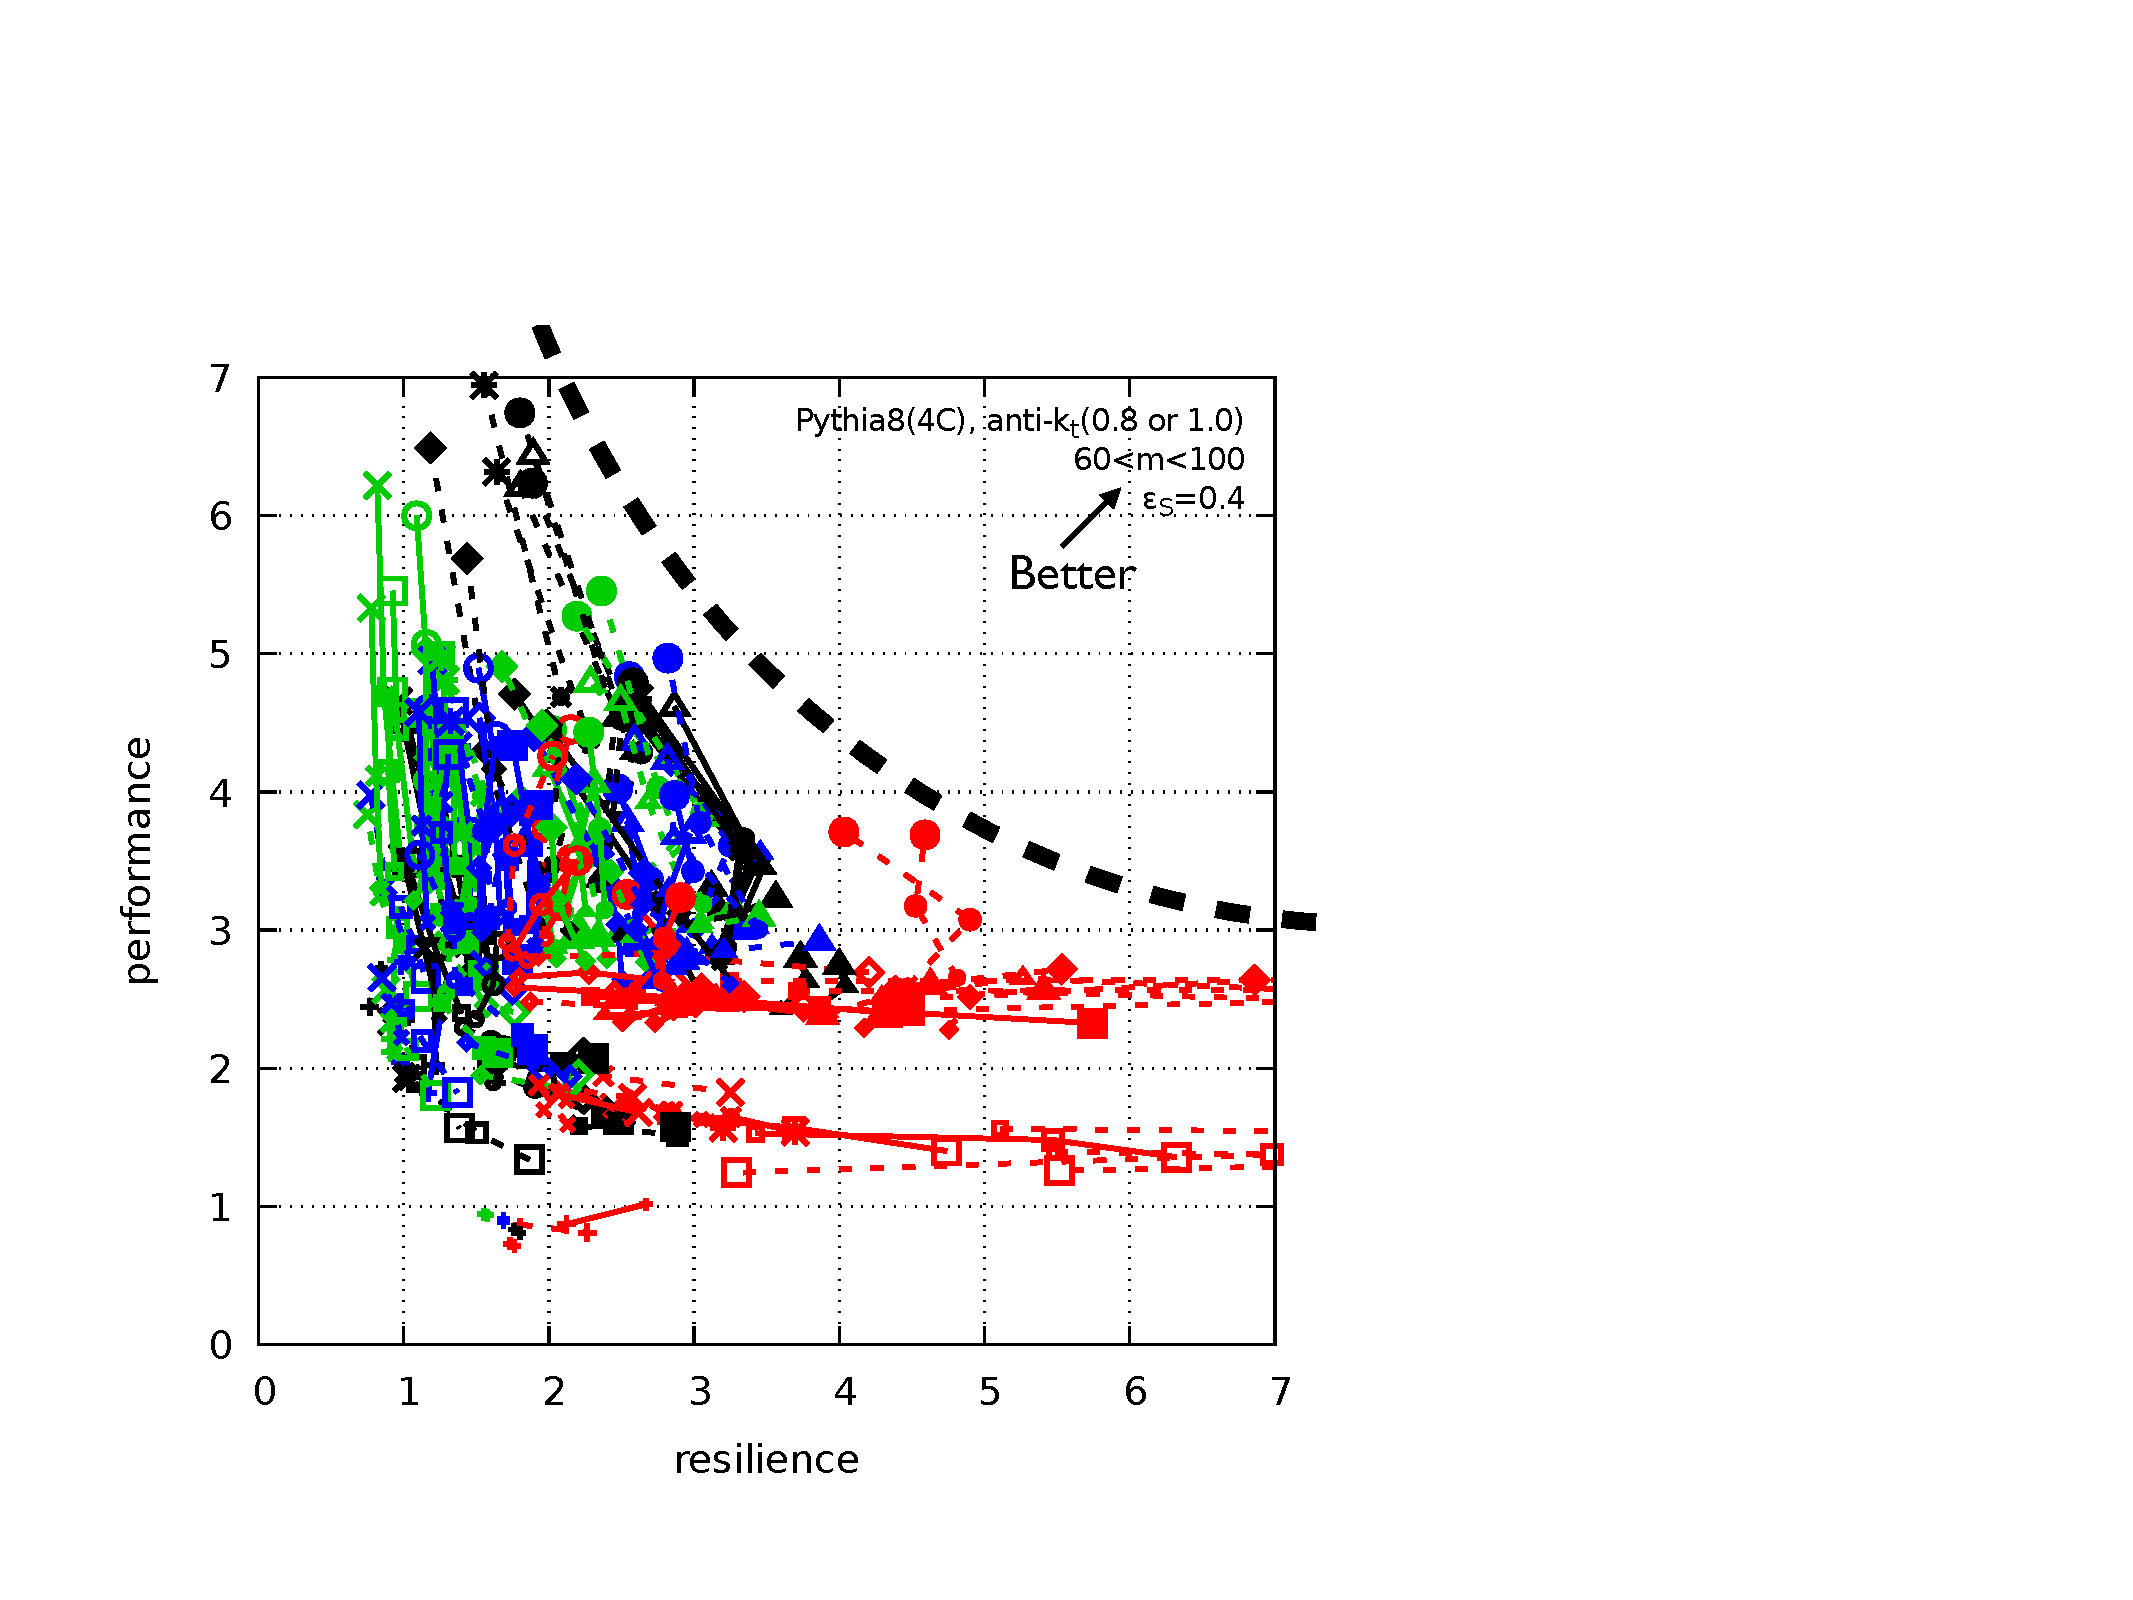
\includegraphics[width=7cm]{figures/gregory_art}
}
\end{center}
\caption{Gregory's Art
}
\label{fig:phasespace}
\end{figure}


%%%%%%%%%%%%%%%%%%%%%%%%%%%%%%%%%%%%%%%
\begin{acknowledgments}
%%%%%%%%%%%%%%%%%%%%%%%%%%%%%%%%%%%%%%%

We thank the participants of Les Houches 2017 for a lively environment and useful discussions.

We also thank \ijm{someone}...

The work of GS is supported in part by the Paris-Saclay IDEX under the
IDEOPTIMALJE grant, by the French Agence Nationale de la Recherche,
under grant ANR-15-CE31-0016, and by the ERC Advanced Grant Higgs@LHC
(No.\ 321133).
%
The work of JT is supported by the DOE under grant contract numbers DE-SC-00012567 and DE-SC-00015476.
%
The work of IM is supported by Office of High Energy Physics of the U.S. Department of Energy under Contract No. DE-AC02-05CH11231, and the LDRD Program of LBNL.


%%%%%%%%%%%%%%%%%%%%%%%%%%%%%%%%%%%%%%%
\end{acknowledgments}
%%%%%%%%%%%%%%%%%%%%%%%%%%%%%%%%%%%%%%%



\appendix

\section{Additional Plots}\label{app:more_plot}

In this appendix we provide additional plots to complement those shown in the text.

\ijm{put some additional plots here}

%\section{Introduction}
%\label{sec:introduction}
%
%Variety of 2-prong taggers, want to understand behavior.  Focus on W bosons.  No b-tagging.  
%
%(3-prong is future)
%
%new physics robustness?
%
%Goals:  understand ATLAS/CMS differences (summary section, it is a byproduct of detector sensitivity, or of truth-level), very high pT behavior,  interplay of jet radius, jet grooming, jet discrimination.  Groomed/ungroomed/dichroic observables.  Detector effects (simplified)
%
%(polarization is separate study?  Or initial study?)
%
%Also interesting in tagging longitudinal vs. transverse W bosons

%\subsection{Brainstorm}
%
%Three dimensional space:  efficiency (performance), NP robustness, detector robustness
%
%1)  Theory-level projection:  efficiency (performance), NP robustness,
%
%both for fixed and variable cuts
%
%we should be able to understand sensitivity (on theory land)
%
%split hadronization and underlying
%
%2)  Experiment:  efficiency vs. detector robustness
%
%
%1) Difference between modern tools on groomed versus ungroomed at truth level  (motivation
%
%2) How affected by pileup/detector effects


%\section{Preliminaries}
%
%\subsection{Event Samples}
%
%WW Pythia 8 pTW > 500 GeV
%
%Need polarized Ws
%
%Need dijet samples
%
%Pileup Samples from pileup study
%
%\subsection{Observables}
%
%CMS:  mMDT mass, ungroomed N2
%ATLAS:  trimmed mass, trimmed D2
%
%\subsection{Detector Simulation}
%
%Do we do DELPHES?
%
%TowerGrid from Peter, included ATLAS/CMS B-field
%
%Calorimetry vs. Particle Flow

%\section{Particle-Level Tagging}
%
%\subsection{Unpolarized Case}
%
%\subsection{Longitudinal versus Transverse Polarization}
%
%\subsection{Adjusting the Jet Radius}
%
%\section{Impact of Detector Effects}
%
%\subsection{Mass Resolution}
%
%\subsection{Tagging Performance}
%
%\subsection{Behavior in the Ultra-boosted Regime}
%
%\section{Comparison of ATLAS and CMS Two-prong Strategies}
%
%
%\section{Conclusions}



\bibliographystyle{jhep}
\bibliography{lh2017_2prong}

\end{document}
